\documentclass[a4paper,12pt]{book}
%\usepackage[a4paper,left=2cm,right=2cm,top=1cm,bottom=1cm,includehead,includefoot,headheight=15pt,heightrounded,footskip=32pt]{geometry}
% Bleed marks, if Warwick Print want them..
\usepackage[paperwidth=230mm,paperheight=317mm,layoutvoffset=10mm,layouthoffset= 10mm,left=2cm,right=2cm,top=1cm,bottom=1cm,includehead,includefoot,headheight=15pt,heightrounded,footskip=36pt,showcrop=true,layout=a4paper]{geometry}
\usepackage{amsmath}
\usepackage{amsfonts}
\usepackage{graphics}
\usepackage{graphicx}
\usepackage[table,xcdraw]{xcolor}
\usepackage[edges]{forest}
\usepackage{float}
\usepackage[pro]{fontawesome5}
\usepackage{ragged2e}
\usepackage{titlesec}
\usepackage{framed}
\usepackage{tikz}
\usepackage{trimclip}
\usepackage{tikz-cd}
\usepackage[printwatermark]{xwatermark}
\usepackage{amssymb}
\usepackage[export]{adjustbox}
\usepackage{tocloft}
\usepackage{etoolbox}
\usepackage{algpseudocode}
\usepackage{fontspec}
\usepackage{pdflscape}
\usepackage{rotating}
\newfontfamily{\fallbackmono}{DejaVu Sans}
\renewcommand{\contentsname}{\normalfont \sffamily \huge \textcolor{id7-aubergine}{Table of Contents}\vspace{-1.25em}}
\renewcommand{\cftsecfont}{\normalfont}
\renewcommand{\cftsecpagefont}{\normalfont}

\setlength{\cftbeforetoctitleskip}{-5pt}
\setlength{\cftaftertoctitleskip}{40pt}
\usetikzlibrary{automata, positioning, shapes.symbols, arrows, chains, calc, shapes.geometric, matrix}
\usepackage{shellesc}
\usepackage{minted}
\usepackage{syntax}
\usemintedstyle{idseven}
\usepackage{listings}
\usepackage[hidelinks]{hyperref}
%\usepackage[osfigures]{opensans}
\usepackage{lastpage}
\usepackage{fancyhdr}
\usepackage{mdframed}
\usepackage{outlines}
\usepackage{bm}
\usepackage{array}
\usepackage{enumitem}
\usepackage[round]{natbib}
\usepackage{environ}
\usepackage{varwidth}
\usepackage{mathtools}
\usepackage{pagecolor}
\usepackage{wrapfig}
\usepackage{nameref}
\usepackage{import}
\usepackage{xifthen}
\usepackage{pdfpages}
\usepackage{transparent}
\setsansfont{Proxima Nova}
\setmonofont{Ubuntu Mono}
\newfontfamily\warwickfont[
Scale=MatchLowercase
%  Path = fonts/
]{Avenir Next}
\makeatletter
\newcommand*{\currentname}{\@currentlabelname}
\makeatother
\usepackage{csquotes}
\usepackage{newfloat}
\usepackage{caption}
\usepackage[super]{nth}
\titleformat{\chapter}[display]
{\normalfont \sffamily \Huge  \color{id7-aubergine}}
{\vspace{-20pt} \flushright \large \color{id7-aubergine} \warwickfont \MakeUppercase { \chaptertitlename \hspace{1 ex} }  { \fontsize{60}{60}\selectfont \color{id7-aubergine} \sffamily  \thechapter }} {0 pt}{\vspace{-40pt}\Huge}
\newlength{\MyMdframedWidthTweak}%
\NewEnviron{MyMdframed}[1][]{%
    \setlength{\MyMdframedWidthTweak}{\dimexpr%
        +\mdflength{innerleftmargin}
        +\mdflength{innerrightmargin}
        +\mdflength{leftmargin}
        +\mdflength{rightmargin}
    }%
    \savebox0{%
        \begin{varwidth}{\dimexpr\linewidth-\MyMdframedWidthTweak\relax}%
            \BODY
        \end{varwidth}%
    }%
    \begin{mdframed}[
        backgroundcolor=lightgrey,
        topline=true,
        rightline=false,
        leftline=false,
        linecolor=id7-aubergine,
        userdefinedwidth=\dimexpr\wd0+\MyMdframedWidthTweak\relax, 
        #1]
        \usebox0
    \end{mdframed}
}

\DeclarePairedDelimiter\abs{\lvert}{\rvert}%
\title{}
\author{}
\definecolor{infogreen}{rgb}{0.153, 0.682, 0.376}
\definecolor{id7-aubergine}{HTML}{5B3069}
\definecolor{id7-gray}{HTML}{3F4246}
\definecolor{body-text}{HTML}{333333}
\definecolor{id7-gold}{HTML}{886C11}
\definecolor{id7-burnt-orange}{HTML}{A14418}
\definecolor{id7-ruby-red}{HTML}{89102C}
\definecolor{id7-emerald-green}{HTML}{797906}
\definecolor{id7-bright-emerald-green}{HTML}{b1e7e1}
\definecolor{id7-sky-blue}{HTML}{204F79}
\definecolor{id7-sky-blue-tint}{HTML}{bccad7}
\definecolor{id7-aubergine-tint}{HTML}{cec1d2}
\definecolor{term-dir}{HTML}{1d7d7d}
\definecolor{term-git}{HTML}{3a5069}
\definecolor{term-green}{HTML}{4c7d1d}
\definecolor{term-branch}{HTML}{8a1818}
\definecolor{skyblue}{rgb}{0.125, 0.31, 0.475}
\setlength{\parindent}{0em}
\setlength{\parskip}{1em}
\definecolor{todocolor}{rgb}{0.688,0.8176,0.93137}
\def\labelitemi{\textcolor{id7-aubergine}{\textbullet}}
\def\labelitemii{\textcolor{id7-aubergine}{\circ}}
\def\labelitemiii{\textcolor{id7-aubergine}{--}}
\definecolor{infogreenlight}{rgb}{0.75,1,0.75}
\newcommand{\todobox}[1] {\colorbox{todocolor}{\parbox{\dimexpr \linewidth-\columnsep}{\vspace{.75\baselineskip}\centering\parbox{0.95\linewidth}{\faIcon{lightbulb} \textbf{TODO:} #1\vspace{.75\baselineskip}}}}}
\newcommand{\readbox}[1] {\colorbox{infogreen}{\parbox{\textwidth}{\vspace{.75\baselineskip}\centering\parbox{0.95\textwidth}{\textcolor{white}{\faicon{book} \textbf{#1}\vspace{.75\baselineskip}}}}}}

\newcommand{\infobox}[1] {\colorbox{id7-bright-emerald-green}{\parbox{\textwidth}{\vspace{.75\baselineskip}\centering\parbox{0.95\textwidth}{\faIcon{info-circle} #1\vspace{.75\baselineskip}}}}}

\newcommand{\boxedfigure}[2]{\begin{MyMdframed}\begin{figure}[H]
            \begin{center}\vspace{2em}\includegraphics[width=0.5\textwidth]{#1}\end{center}
            \caption{#2}
\end{figure}\end{MyMdframed}}

\newcommand{\widthboxedfigure}[3]{\begin{MyMdframed}\begin{figure}[H]
            \begin{center}\vspace{2em}\includegraphics[width=#3\textwidth]{#1}\end{center}
            \caption{#2}
\end{figure}\end{MyMdframed}}

\newcommand{\infoinlineicon}[1] {\colorbox{infogreenlight}{\faicon{info-circle} #1}}

\newcommand{\infoinline}[1] {\colorbox{infogreenlight}{#1}}

\definecolor{orange}{rgb}{0.9529,0.85176,0.5070588}

\newcommand{\warnbox}[1] {\colorbox{orange}{\parbox{\textwidth}{\vspace{.75\baselineskip}\centering\parbox{0.95\textwidth}{\faicon{exclamation-triangle} #1\vspace{.75\baselineskip}}}}}

\newcommand{\warninlineicon}[1] {\colorbox{orange}{\faicon{exclamation-triangle} #1}}

\makeatletter
\let\old@rule\@rule
\def\@rule[#1]#2#3{\textcolor{lightgrey}{\old@rule[#1]{#2}{#3}}}
\makeatother

\newcommand{\warninline}[1] {\colorbox{orange}{#1}}
\usepackage{emptypage}
\titleformat{\section}
{\normalfont\sffamily\huge\color{id7-aubergine}}
{\thesection. }{0em}{}

\titleformat{\subsection}
{\normalfont\Large\sffamily\color{id7-aubergine}}
{\thesubsection. }{0em}{}

\titleformat{\subsubsection}
{\normalfont\large\sffamily\color{id7-aubergine}}
{\thesubsubsection. }{0em}{}
\fancyhf{}
\pagestyle{fancy}

\renewcommand{\headrulewidth}{0pt}
\lfoot{\textcolor{grey}{Adam Williams}}
\rfoot{\textcolor{grey}{Page \thepage{} of \pageref{LastPage}}}

\renewcommand*\footnoterule{\hspace{-3.1cm}\noindent\makebox[\paperwidth]{
\includegraphics[width=230mm]{divider}}}

% Redefine the plain page style
%\fancypagestyle{plain}{%
%    \fancyhf{}%
%    \fancyhead[L]{\textcolor{grey}{\thedate}}%
%    \fancyhead[R]{\textcolor{grey}{\currentname}}%
%    \fancyfoot[L]{\textcolor{grey}{Adam Williams}}%
%    \fancyfoot[R]{\textcolor{grey}{Page \thepage{} of \pageref{LastPage}}}%
%    \renewcommand{\headrulewidth}{0pt}% Line at the header invisible
%    \renewcommand{\footrulewidth}{0pt}% Line at the footer visible
%}
\definecolor{grey}{rgb}{0.5,0.5,0.5}
\definecolor{dgrey}{rgb}{0.25,0.25,0.25}
\definecolor{lightgrey}{rgb}{0.96,0.96,0.96}

\def \spacedrule {\textcolor{id7-aubergine}{\hrule}\vspace{1em}}
\def \thedate {\today}
\lhead{\textcolor{grey}{\thedate}}
\rhead{\textcolor{grey}{\currentname}}


% Set up example boxes

\newenvironment{example}[1]
{
        \begin{mdframed} \setlength{\parskip}{1em}
            \vspace{0.5em}
            \sffamily \textcolor{id7-aubergine}{\faPuzzlePiece{} \textbf{Example:} #1}
            \vspace{0.5em}
            \rmfamily

            }
            {\end{mdframed}
}

% And algorithm boxes

\DeclareFloatingEnvironment[fileext=frm,placement={!ht},name=Algorithm]{algorithmflt}
\captionsetup[figure]{name=\faImage{} Figure, singlelinecheck=false,font={color=id7-aubergine,sf},position=top,labelfont=bf}
\newcounter{algorithm}
\newenvironment{algbox}[1]
{
        \begin{mdframed} \setlength{\parskip}{1em}
            \vspace{1.5em}

            \captionsetup[algorithmflt]{name=\faCogs{} Algorithm, singlelinecheck=false,font={color=id7-aubergine,sf},position=top}
            \captionof{algorithmflt}{#1}\hfill

            \rmfamily
            \captionsetup{style=default}

        }
        {\vspace{0.5em}\end{mdframed}
}

% And code boxes

\DeclareFloatingEnvironment[fileext=frm,placement={!ht},name=Code Listing]{codeflt}
\captionsetup[algorithmflt]{labelfont=bf}
\captionsetup[figure]{labelfont=bf}
\renewcommand{\theFancyVerbLine}{\rmfamily \textcolor[rgb]{0.7, 0.7, 0.7}{\arabic{FancyVerbLine}}}

\newenvironment{mycode}[4][]
{\VerbatimEnvironment
    \begin{codeflt}[tb]\begin{mdframed}
        \captionsetup{name=\faIcon{brackets-curly} \textbf{Code Listing}, singlelinecheck=false,font={color=id7-aubergine,sf},position=top}
        \vspace{0.5em}
        \caption{#3 \hfill #4}
        \vspace{0.5em}
        \captionsetup{style=default}
    \begin{minted}[#1]{#2}}
    {\end{minted}\vspace{0.5em}\end{mdframed}\end{codeflt}}

\newenvironment{mycodefile}[5][]
{\begin{mdframed}
            \vspace{0.5em}
            \sffamily \textcolor{id7-aubergine}{\faIcon{brackets-curly} \textbf{Code Listing} #3 \hfill #4}
            \rmfamily
            \inputminted{#2}{#5}}
            {\vspace{0.5em}\end{mdframed}}

% Abstract and keywords
\newenvironment{abstract}{\centering{\normalfont\Large\sffamily\color{id7-aubergine}Abstract}\vspace{0.3cm}\\
    \hfill\begin{minipage}{0.95\textwidth}
        \rule{\textwidth}{1pt}}
    {\par\noindent\rule{\textwidth}{1pt}\end{minipage}}

\newenvironment{keywords}{\centering{\normalfont\Large\sffamily\color{id7-aubergine}Keywords}\vspace{0.3cm}\\
    \hfill\begin{minipage}{0.95\textwidth}
        \rule{\textwidth}{1pt}}
    {\par\noindent\rule{\textwidth}{1pt}\end{minipage}}

\renewenvironment{leftbar}[2][\hsize]
{
    \def\FrameCommand
    {
        {\color{#2}\vrule width 3pt}
        \hspace{0pt}
    }
    \MakeFramed{\hsize#1\advance\hsize-\width\FrameRestore}
}
{\endMakeFramed}

\newcommand{\termbox}[1] {\colorbox{lightgrey}{\parbox{\textwidth}{\vspace{.75\baselineskip}\centering\parbox{0.95\textwidth}{ \sffamily#1\vspace{.75\baselineskip}}}}}
%isolated term
%#1 - Optional. Space between node and grouping line. Default=0
%#2 - node
%#3 - filling color
\newcommand{\implicantsol}[3][0]{
    \draw[rounded corners=3pt, fill=#3, opacity=0.3] ($(#2.north west)+(135:#1)$) rectangle ($(#2.south east)+(-45:#1)$);
    }


%internal group
%#1 - Optional. Space between node and grouping line. Default=0
%#2 - top left node
%#3 - bottom right node
%#4 - filling color
\newcommand{\implicant}[4][0]{
    \draw[rounded corners=3pt, fill=#4, opacity=0.3] ($(#2.north west)+(135:#1)$) rectangle ($(#3.south east)+(-45:#1)$);
    }

%group lateral borders
%#1 - Optional. Space between node and grouping line. Default=0
%#2 - top left node
%#3 - bottom right node
%#4 - filling color
\newcommand{\implicantcostats}[4][0]{
    \draw[rounded corners=3pt, fill=#4, opacity=0.3] ($(rf.east |- #2.north)+(90:#1)$)-| ($(#2.east)+(0:#1)$) |- ($(rf.east |- #3.south)+(-90:#1)$);
    \draw[rounded corners=3pt, fill=#4, opacity=0.3] ($(cf.west |- #2.north)+(90:#1)$) -| ($(#3.west)+(180:#1)$) |- ($(cf.west |- #3.south)+(-90:#1)$);
}

%group top-bottom borders
%#1 - Optional. Space between node and grouping line. Default=0
%#2 - top left node
%#3 - bottom right node
%#4 - filling color
\newcommand{\implicantdaltbaix}[4][0]{
    \draw[rounded corners=3pt, fill=#4, opacity=0.3] ($(cf.south -| #2.west)+(180:#1)$) |- ($(#2.south)+(-90:#1)$) -| ($(cf.south -| #3.east)+(0:#1)$);
    \draw[rounded corners=3pt, fill=#4, opacity=0.3] ($(rf.north -| #2.west)+(180:#1)$) |- ($(#3.north)+(90:#1)$) -| ($(rf.north -| #3.east)+(0:#1)$);
}

%group corners
%#1 - Optional. Space between node and grouping line. Default=0
%#2 - filling color
\newcommand{\implicantcantons}[2][0]{
    \draw[rounded corners=3pt, opacity=.3] ($(rf.east |- 0.south)+(-90:#1)$) -| ($(0.east |- cf.south)+(0:#1)$);
    \draw[rounded corners=3pt, opacity=.3] ($(rf.east |- 8.north)+(90:#1)$) -| ($(8.east |- rf.north)+(0:#1)$);
    \draw[rounded corners=3pt, opacity=.3] ($(cf.west |- 2.south)+(-90:#1)$) -| ($(2.west |- cf.south)+(180:#1)$);
    \draw[rounded corners=3pt, opacity=.3] ($(cf.west |- 10.north)+(90:#1)$) -| ($(10.west |- rf.north)+(180:#1)$);
    \fill[rounded corners=3pt, fill=#2, opacity=.3] ($(rf.east |- 0.south)+(-90:#1)$) -|  ($(0.east |- cf.south)+(0:#1)$) [sharp corners] ($(rf.east |- 0.south)+(-90:#1)$) |-  ($(0.east |- cf.south)+(0:#1)$) ;
    \fill[rounded corners=3pt, fill=#2, opacity=.3] ($(rf.east |- 8.north)+(90:#1)$) -| ($(8.east |- rf.north)+(0:#1)$) [sharp corners] ($(rf.east |- 8.north)+(90:#1)$) |- ($(8.east |- rf.north)+(0:#1)$) ;
    \fill[rounded corners=3pt, fill=#2, opacity=.3] ($(cf.west |- 2.south)+(-90:#1)$) -| ($(2.west |- cf.south)+(180:#1)$) [sharp corners]($(cf.west |- 2.south)+(-90:#1)$) |- ($(2.west |- cf.south)+(180:#1)$) ;
    \fill[rounded corners=3pt, fill=#2, opacity=.3] ($(cf.west |- 10.north)+(90:#1)$) -| ($(10.west |- rf.north)+(180:#1)$) [sharp corners] ($(cf.west |- 10.north)+(90:#1)$) |- ($(10.west |- rf.north)+(180:#1)$) ;
}

%Empty Karnaugh map 4x4
\newenvironment{Karnaugh}%
{
\begin{tikzpicture}[baseline=(current bounding box.north),scale=0.8]
\draw (0,0) grid (4,4);
\draw (0,4) -- node [pos=0.7,above right,anchor=south west] {cd} node [pos=0.7,below left,anchor=north east] {ab} ++(135:1);
%
\matrix (mapa) [matrix of nodes,
        column sep={0.8cm,between origins},
        row sep={0.8cm,between origins},
        every node/.style={minimum size=0.3mm},
        anchor=8.center,
        ampersand replacement=\&] at (0.5,0.5)
{
                       \& |(c00)| 00         \& |(c01)| 01         \& |(c11)| 11         \& |(c10)| 10         \& |(cf)| \phantom{00} \\
|(r00)| 00             \& |(0)|  \phantom{0} \& |(1)|  \phantom{0} \& |(3)|  \phantom{0} \& |(2)|  \phantom{0} \&                     \\
|(r01)| 01             \& |(4)|  \phantom{0} \& |(5)|  \phantom{0} \& |(7)|  \phantom{0} \& |(6)|  \phantom{0} \&                     \\
|(r11)| 11             \& |(12)| \phantom{0} \& |(13)| \phantom{0} \& |(15)| \phantom{0} \& |(14)| \phantom{0} \&                     \\
|(r10)| 10             \& |(8)|  \phantom{0} \& |(9)|  \phantom{0} \& |(11)| \phantom{0} \& |(10)| \phantom{0} \&                     \\
|(rf) | \phantom{00}   \&                    \&                    \&                    \&                    \&                     \\
};
}%
{
\end{tikzpicture}
}

%Empty Karnaugh map 2x4
\newenvironment{Karnaughvuit}%
{
\begin{tikzpicture}[baseline=(current bounding box.north),scale=0.8]
\draw (0,0) grid (4,2);
\draw (0,2) -- node [pos=0.7,above right,anchor=south west] {bc} node [pos=0.7,below left,anchor=north east] {a} ++(135:1);
%
\matrix (mapa) [matrix of nodes,
        column sep={0.8cm,between origins},
        row sep={0.8cm,between origins},
        every node/.style={minimum size=0.3mm},
        anchor=4.center,
        ampersand replacement=\&] at (0.5,0.5)
{
                      \& |(c00)| 00         \& |(c01)| 01         \& |(c11)| 11         \& |(c10)| 10         \& |(cf)| \phantom{00} \\
|(r00)| 0             \& |(0)|  \phantom{0} \& |(1)|  \phantom{0} \& |(3)|  \phantom{0} \& |(2)|  \phantom{0} \&                     \\
|(r01)| 1             \& |(4)|  \phantom{0} \& |(5)|  \phantom{0} \& |(7)|  \phantom{0} \& |(6)|  \phantom{0} \&                     \\
|(rf) | \phantom{00}  \&                    \&                    \&                    \&                    \&                     \\
};
}%
{
\end{tikzpicture}
}

%Empty Karnaugh map 2x2
\newenvironment{Karnaughquatre}%
{
\begin{tikzpicture}[baseline=(current bounding box.north),scale=0.8]
\draw (0,0) grid (2,2);
\draw (0,2) -- node [pos=0.7,above right,anchor=south west] {b} node [pos=0.7,below left,anchor=north east] {a} ++(135:1);
%
\matrix (mapa) [matrix of nodes,
        column sep={0.8cm,between origins},
        row sep={0.8cm,between origins},
        every node/.style={minimum size=0.3mm},
        anchor=2.center,
        ampersand replacement=\&] at (0.5,0.5)
{
          \& |(c00)| 0          \& |(c01)| 1  \\
|(r00)| 0 \& |(0)|  \phantom{0} \& |(1)|  \phantom{0} \\
|(r01)| 1 \& |(2)|  \phantom{0} \& |(3)|  \phantom{0} \\
};
}%
{
\end{tikzpicture}
}

%Defines 8 or 16 values (0,1,X)
\newcommand{\contingut}[1]{%
\foreach \x [count=\xi from 0]  in {#1}
     \path (\xi) node {\x};
}

%Places 1 in listed positions
\newcommand{\minterms}[1]{%
    \foreach \x in {#1}
        \path (\x) node {1};
}

%Places 0 in listed positions
\newcommand{\maxterms}[1]{%
    \foreach \x in {#1}
        \path (\x) node {0};
}

%Places X in listed positions
\newcommand{\indeterminats}[1]{%
    \foreach \x in {#1}
        \path (\x) node {X};
}
\newsavebox\mybox
\savebox\mybox{\tikz[color=id7-aubergine,opacity=0.3]\node{\sffamily DRAFT 1};}
%\newwatermark*[
%allpages,
%angle=45,
%scale=6,
%xpos=-20,
%ypos=15,
%]{\usebox\mybox}

% Try and avoid *stupid* hypthenation
% SE https://tex.stackexchange.com/a/335088/102207
\pretolerance=5000
\tolerance=9000
\emergencystretch=0pt
\righthyphenmin=4
\lefthyphenmin=4

% Don't stretch pages vertically, it looks shit
\raggedbottom

\renewcommand\arraystretch{1.5}
\DeclareMathSymbol{\mlq}{\mathord}{operators}{``}
\DeclareMathSymbol{\mrq}{\mathord}{operators}{`'}

% ======================

\begin{document}
  
\newgeometry{margin=0in,showcrop=true}
\begin{titlepage}
    
    \tikz[remember picture,overlay] \node[opacity=1,inner sep=0pt] at (current page.center){
\includegraphics[width=\paperwidth,height=\paperheight]{bg.eps}};
    \vspace{0.6\textheight} % height of the devil
    
    {\hspace{0pt}\vspace{0pt}\begin{tikzpicture}[scale=\paperwidth/1cm, overlay]
        \filldraw[draw=none,fill=white]
        (0, 0)
        -- (0.65838,0) 
        -- (0.71534285714,-0.1) 
        -- (0.7577,-0.0215)
        -- (0.8001, -0.1)
        -- (0.8571,0)
        -- (1, 0)
        -- (1, -0.5)
        -- (0, -0.5);
        
        \node[opacity=1,inner sep=0pt] at (0.7577, -0.15){
\includegraphics[width=6cm]{logotype}};
        \node[text width=15cm] at (0.39,-0.15) {\warwickfont\fontsize{40}{10}\selectfont\textcolor{id7-aubergine}{Regular Expression\\\vspace{0.2cm}Refinement Types}};
        \end{tikzpicture}}
    
    {\par}
    \vspace{1.25cm}
    \vspace{3.5cm}
    {\hspace{1.56cm}\Huge \warwickfont Project Report}
    \vspace{0.16cm}
    {\par}
    {\hspace{1.60cm}\large \warwickfont Adam Williams (3\textsuperscript{rd} year Computer Science)}


    {\hspace{1.60cm}\large \warwickfont Michael Gale (supervisor)}
    \vfill
\end{titlepage}
\restoregeometry
\restorepagecolor

\tableofcontents
\pagebreak[5]
\vspace{2em}
\section*{Acknowledgements}

I would like to thank my supervisor, Michael Gale, for his advice throughout this project and for shaping its
direction from the beginning. His feedback has always been comprehensive and insightful, and his dedication to
both teaching and supervision is clear to me.

Next, I wish to thank my former colleagues at MWR InfoSecurity. In particular: Kostas Lintovois, my mentor during
my time at MWR, taught me a great deal about practical security assurance work and cemented my knowledge of some of the
motivating vulnerabilities we discuss in this report. Donato Capitella and James Coote were a pleasure to work with
throughout the course of our project creating a platform for security-focussed training ``labs''--a project which
greatly improved my knowledge of software engineering.
And finally, thanks to the various consultants I worked with in the office and on-site: Mohit, James, Dennis, Alex, Amar,
Connor and many others.

Within Warwick, I am grateful to Mat Mannion and the teams within IT Services for their support of
my security work and exposing me to a range of new programming languages and technologies.

Whilst often overlooked, formatting is an essential part of any report, and I must gratefully acknowledge I have
received from the TeX.SX community and \LaTeX{} package maintainers who have answered my numerous questions.

Lastly, sincere thanks are due to my friends and family for their support during the year.

\pagebreak[5]
\begin{keywords}
    Type Systems, Refinement Types, Application Security, User Input, Satisfiability Modulo Theories,
    Programming Languages, Static Analysis
\end{keywords}

\vspace{0.5em}

\begin{abstract}
    Entire classes of modern web application vulnerabilities arise due to problematic user input handling.
    This includes cross-site scripting (XSS), \emph{injection} issues (SQL, LDAP, etc.), insecure deserialisation and
    file inclusion vulnerabilities – all of which are encountered by information security firms on a regular basis in application assessments.
    This project explores the use of regular expressions as refinement types for constrained data in order to model user input validation.
    We formalise the type system of such a language and implement it.
    We then compare our system to and evaluate it against other, existing approaches by considering false positive and negative rates with a series of test cases.
\end{abstract}
\titlespacing*{\chapter}
{0pt}{0pt}{2.0ex}

\chapter{Introduction}
Over the last decade, use of web and thick client applications globally has greatly increased.
People increasingly access services online--to manage their finances \citep{jayawardhena2000changes}, use government
services \citep{fox2010directgov} and communicate using social media \citep{boulianne2015social}.
On a daily basis users entrust these systems with maintaining the privacy of their personal information and safeguarding
their finances.
With the transition from a web centred primarily around exchanging documents to a platform for deploying complex
applications, security is increasingly important.

\section{Application Security}

Application security is of particular interest because it transcends the underlying infrastructure on which applications
are deployed.
Despite the popularity of cloud IaaS (infrastructure-as-a-service) and PaaS (platform-as-a-service)
offerings which can substantially improve infrastructure security, applications will continue to be vulnerable.

The predominant cause of these vulnerabilities is improper user input handling \citep{schneier2011secrets}.
The \emph{Open Web Application Security Project} (OWASP) regularly publishes a list of the top ten most critical
security issues, and a subset of these are described below \citep{owasp10}:

\begin{description}
    \item[Injection] Covers query injection, where user input is improperly interpolated into a e.g. database Structured
                     Query Language (SQL) query or a directory LDAP search. Malicious user input can retrieve or modify
                     sensitive data, bypass authorisation controls and (in some cases) run arbitrary code \citep[p.~291]{stuttard2011web}.
    \item[Broken Access Control] Covers vulnerabilities such as insecure direct object access (IDOR) where authorisation
                                 checks are not implemented consistently and the user's request is trusted in one or
                                 more parts of the application \citep[p.~257]{stuttard2011web}. Also includes path
                                 traversal vulnerabilities where user input is used to construct a filesystem path and a
                                 malicious actor can include e.g. \texttt{../} to traverse up one level.
    \item[XML External Entities (XXE)] A vulnerability which involves improperly handling user encoded in the XML
                                       interchange format. XML supports functionality to reference entities from an
                                       external location. Exploitation may allow arbitrary files to be read, sensitive
                                       data to be exposed or code to be executed  \citep[p.~384]{stuttard2011web}.
    \item[Cross-Site Scripting (XSS)] When user input is not properly handled in the context of a HTML web page or
                                      inside JavaScript, a user can provide malicious input that can run arbitrary code
                                      on the client. This can be used by an attacker to steal or misuse a victim's
                                      session \citep[p.~431]{stuttard2011web}.
    \item[Insecure Deserialization] Results from insecurely converting user input into a language object.
\end{description}

Many of these vulnerabilities--and the necessary techniques for preventing them--have been well-established for a
number of years, and yet they continue to be regularly discovered in production applications \citep[p.~2]{schneier2011secrets}.

\subsection{Examples}\label{subsec:examples}

From the above classes of vulnerabilities, we will focus on a subset of motivating examples.
In the context of a Java Enterprise Edition (EE) application these will include SQL injection, LDAP injection and
path traversal.

\subsubsection{SQL Injection}
\label{ex:sqli}

Structured Query Language (SQL) is used with relational database systems to create, retrieve, update and delete data.
SQL injection falls into the \emph{injection} category of vulnerabilities above.
Generally, it arises when SQL queries concatenate or interpolate user input into a query command.
An attacker is able to craft user input that ``breaks out'' of e.g. a string literal and execute arbitrary SQL.
This could lead to exfiltration of sensitive data, destruction of data or violation of data integrity.
SQL injection is typically mitigated using \emph{prepared statements} \citep{stuttard2011web}, which allow placeholders to be set-up in the
query and then bound to meaningful values at execution time.
By using this technique to bind user input to specific placeholders, the possibility to inject SQL is removed.

The example below shows a Java function, \texttt{lookupUserNameByToken}, which performs a query to retrieve data from
a \textsc{Users} table based on a user-provided \texttt{token} argument.
Instead of using a prepared statement, once the query is created, the token input is concatenated directly into the
\textcolor{id7-aubergine}{where} clause.

\newsavebox\myv

\begin{lrbox}{\myv}\begin{minipage}{\textwidth}
\begin{minted}[fontsize=\fontsize{0.01pt}{0.01pt}]{java}
public String lookupUserNameByToken(String token) throws SQLException {
    Statement stmt = connection.createStatement();
    String query = "select * from Users where ";
    query += "token = '" + token + "'";
    ResultSet rs = stmt.executeQuery(sql);
    if (rs.next()) {
        return rs.getString("name");
    }
    return null;
}
\end{minted}
\end{minipage}\end{lrbox}

\begin{mdframed}[backgroundcolor=lightgrey]
\begin{Verbatim}[commandchars=\\\{\}]
\PYGidseven{k+kd}{public} \PYGidseven{n}{String} \PYGidseven{n+nf}{lookupUserNameByToken}\PYGidseven{o}{(}\PYGidseven{n}{String} \PYGidseven{n}{token}\PYGidseven{o}{)} \PYGidseven{k+kd}{throws} \PYGidseven{n}{SQLException} \PYGidseven{o}{\PYGidsevenZob{}}
    \PYGidseven{n}{Statement} \PYGidseven{n}{stmt} \PYGidseven{o}{=} \PYGidseven{n}{connection}\PYGidseven{o}{.}\PYGidseven{n+na}{createStatement}\PYGidseven{o}{(}\PYGidseven{o}{)}\PYGidseven{o}{;}
    \PYGidseven{n}{String} \PYGidseven{n}{query} \PYGidseven{o}{=} \PYGidseven{l+s}{\PYGidsevenZdq{}select * from users where \PYGidsevenZdq{}}\PYGidseven{o}{;}
    \colorbox{id7-ruby-red}{\textcolor{white}{\faExclamationTriangle{} \PYGidseven{n}{query} \PYGidseven{o}{+=} \PYGidsevenZdq{} token = '\PYGidsevenZdq{} \PYGidseven{o}{+} \PYGidseven{n}{token} \PYGidseven{o}{+} \PYGidsevenZdq{}'\PYGidsevenZdq{} \PYGidseven{o}{;}}}
    \PYGidseven{n}{ResultSet} \PYGidseven{n}{rs} \PYGidseven{o}{=} \PYGidseven{n}{stmt}\PYGidseven{o}{.}\PYGidseven{n+na}{executeQuery}\PYGidseven{o}{(}\PYGidseven{n}{query}\PYGidseven{o}{)}\PYGidseven{o}{;}
    \PYGidseven{k}{if} \PYGidseven{o}{(}\PYGidseven{n}{rs}\PYGidseven{o}{.}\PYGidseven{n+na}{next}\PYGidseven{o}{(}\PYGidseven{o}{)}\PYGidseven{o}{)} \PYGidseven{o}{\PYGidsevenZob{}}
        \PYGidseven{k}{return} \PYGidseven{n}{rs}\PYGidseven{o}{.}\PYGidseven{n+na}{getString}\PYGidseven{o}{(}\PYGidseven{l+s}{\PYGidsevenZdq{}name\PYGidsevenZdq{}}\PYGidseven{o}{)}\PYGidseven{o}{;}
    \PYGidseven{o}{\PYGidsevenZcb{}}
    \PYGidseven{k}{return} \PYGidseven{k+kc}{null}\PYGidseven{o}{;}
\PYGidseven{o}{\PYGidsevenZcb{}}
\end{Verbatim}
\end{mdframed}

An attacker able to directly specify a token, could provide an input string containing a single quote \texttt{'}
character to break out of the string literal in the query.

For instance, providing a token \texttt{' or 1=1 --} would create the following query:

\begin{minted}{sql}
select * from Users where token = '' or 1=1 -- '
\end{minted}

\infobox{
The \texttt{--} token is used to create a comment until the end of the query.
This ensures no syntax error is introduced when the Java code ends the string after appending the user input.}

This query would return all users in the database.

\subsubsection{LDAP Injection}

The Lightweight Directory Access Protocol (LDAP) is a networked protocol designed for querying directory services.
These services are used for storing and organising network entities, such as users and devices.
Microsoft's Active Directory (AD) is a commonly deployed enterprise solution for storing user information and handling
network authentication.

\begin{figure}[H]
    \begin{MyMdframed}
        \vspace{0.5em}


        \caption{\label{figure:wso}LDAP is used internally at Warwick to power the single sign-on system}
        \vspace{0.5em}
        \captionsetup{style=default}
        \begin{center}
            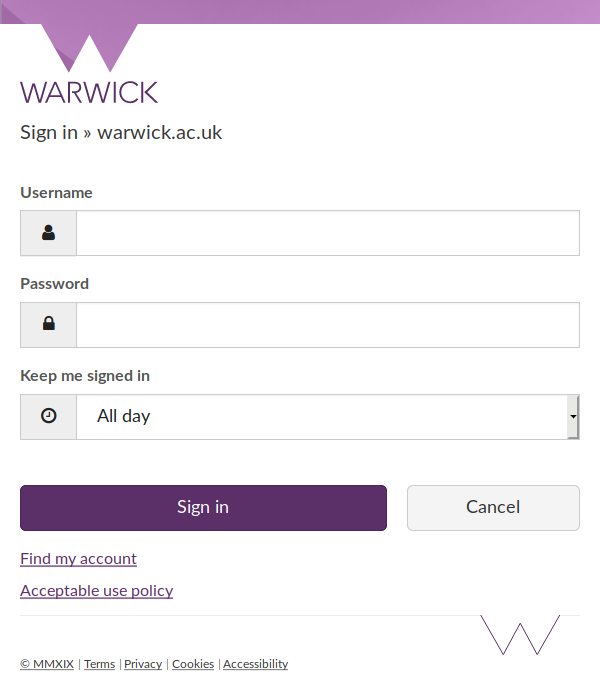
\includegraphics[width=0.5\linewidth]{wso.png}
        \end{center}
    \end{MyMdframed}
\end{figure}

LDAP queries are written in a compact manner using symbols for each operation and parentheses for each clause:

\texttt{(\&(warwickUniId=1510654)(sn=Williams))}

This query retrieves the user with attribute \texttt{warwickUniId} set to value 1510654 \emph{and} surname (sn) set to value
``Williams''.
The \texttt{\&} operator specifies conjunction to be applied to the nested filters.

Much like SQL injection, LDAP injection arises when user-input is concatenated into a filter name or value:

\newsavebox\myva
\begin{lrbox}{\myva}\begin{minipage}{\textwidth}
    \begin{mycodefile}{csharp}{\label{code:motivating:ldap:1}A vulnerable LDAP query function}{C\#}{ldap.cs}\end{mycodefile}
\end{minipage}\end{lrbox}

\begin{mdframed}[backgroundcolor=lightgrey]
\begin{Verbatim}[commandchars=\\\{\}]
\PYGidseven{k}{public} \PYGidseven{k+kt}{string} \PYGidseven{n+nf}{GetSurnameForUser}\PYGidseven{p}{(}\PYGidseven{k+kt}{string} \PYGidseven{n}{username}\PYGidseven{p}{)}
\PYGidseven{p}{\PYGidsevenZob{}}
    \PYGidseven{k+kt}{var} \PYGidseven{n}{directoryEntry} \PYGidseven{p}{=} \PYGidseven{k}{new} \PYGidseven{n}{DirectoryEntry}\PYGidseven{p}{(}\PYGidseven{l+s}{\PYGidsevenZdq{}LDAP://acme.corp\PYGidsevenZdq{}}\PYGidseven{p}{);}
    \PYGidseven{k+kt}{var} \PYGidseven{n}{searcher} \PYGidseven{p}{=} \PYGidseven{k}{new} \PYGidseven{n}{DirectorySearcher}\PYGidseven{p}{(}\PYGidseven{n}{directoryEntry}\PYGidseven{p}{);}
    \colorbox{id7-ruby-red}{\textcolor{white}{\faExclamationTriangle{} searcher.Filter = \PYGidsevenZdq{}(cn=\PYGidsevenZdq{} + username + \PYGidsevenZdq{})\PYGidsevenZdq{};}}
    \PYGidseven{k+kt}{var} \PYGidseven{n}{result} \PYGidseven{p}{=} \PYGidseven{n}{searcher}\PYGidseven{p}{.}\PYGidseven{n}{FindOne}\PYGidseven{p}{();}
    \PYGidseven{k}{return} \PYGidseven{n}{result}\PYGidseven{p}{.}\PYGidseven{n}{Properties}\PYGidseven{p}{[}\PYGidseven{l+s}{\PYGidsevenZdq{}sn\PYGidsevenZdq{}}\PYGidseven{p}{][}\PYGidseven{l+m}{0}\PYGidseven{p}{].}\PYGidseven{n}{ToString}\PYGidseven{p}{();}
\PYGidseven{p}{\PYGidsevenZcb{}}
\end{Verbatim}
\end{mdframed}

The impact is generally more limited, but due to the support for wildcard characters it is possible to leak other
attribute values by testing for a character at a time.
Numeric values or dates can be exfiltrated using a binary search approach.

\begin{figure}[H]
    \begin{MyMdframed}
        \vspace{0.5em}


        \caption{Injection into a conjunctive query can be used to exfiltrate data}
        \vspace{0.5em}
        \captionsetup{style=default}

        \begin{center}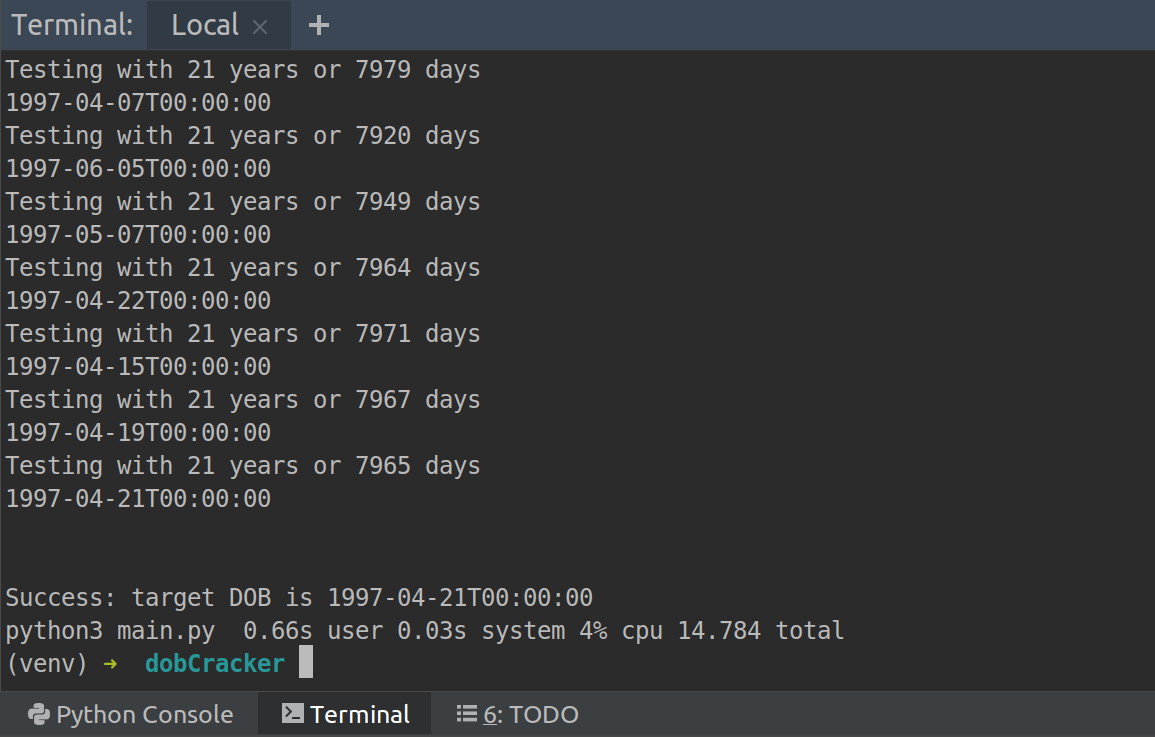
\includegraphics[width=0.5\linewidth]{dobcrack.png}\end{center}

        \vspace{0.5em}

        Note that despite network latency, we can still leak a value in a short period of time (< 15s) by
        repeatedly querying an oracle with less than/greater than filters and observing the response.
    \end{MyMdframed}
\end{figure}

The best practice for mitigating this vulnerability involves using an encoder that is able to escape LDAP control
characters (for example, right parenthesis is replaced with \texttt{\textbackslash 29}).
This ensures that user input is then not considered part of a query.

\subsubsection{Path Traversal}

Many applications read and write files to the filesystem.
Problems arise when user input is permitted to influence the destination path.

Consider a Java function which is designed to persist user preference information in a text file:

\newsavebox\myvb
\begin{lrbox}{\myvb}\begin{minipage}{\textwidth}
\begin{mycodefile}{java}{Hidden}{Java}{pathtraversal.java}\end{mycodefile}
\end{minipage}\end{lrbox}

\begin{mdframed}
\begin{Verbatim}[commandchars=\\\{\}]
\PYGidseven{k+kd}{public} \PYGidseven{k+kd}{static} \PYGidseven{k+kt}{void} \PYGidseven{n+nf}{writeUserPreference}\PYGidseven{o}{(}\PYGidseven{n}{String} \PYGidseven{n}{username}\PYGidseven{o}{,} \PYGidseven{n}{Preference} \PYGidseven{n}{pref}\PYGidseven{o}{)} \PYGidseven{o}{\PYGidsevenZob{}}
    \PYGidseven{k}{try} \PYGidseven{o}{\PYGidsevenZob{}}
        \colorbox{id7-ruby-red}{\textcolor{white}{\faExclamationTriangle{} String path = \PYGidsevenZdq{}/tmp/prefs/\PYGidsevenZdq{} + username;}}
        \PYGidseven{n}{Files}\PYGidseven{o}{.}\PYGidseven{n+na}{writeString}\PYGidseven{o}{(}\PYGidseven{n}{Paths}\PYGidseven{o}{.}\PYGidseven{n+na}{get}\PYGidseven{o}{(}\PYGidseven{n}{path}\PYGidseven{o}{),} \PYGidseven{n}{pref}\PYGidseven{o}{.}\PYGidseven{n+na}{toString}\PYGidseven{o}{());}
    \PYGidseven{o}{\PYGidsevenZcb{}} \PYGidseven{k}{catch}\PYGidseven{o}{(}\PYGidseven{n}{IOException} \PYGidseven{n}{e}\PYGidseven{o}{)} \PYGidseven{o}{\PYGidsevenZob{}}
        \PYGidseven{n}{e}\PYGidseven{o}{.}\PYGidseven{n+na}{printStackTrace}\PYGidseven{o}{();}
    \PYGidseven{o}{\PYGidsevenZcb{}}
\PYGidseven{o}{\PYGidsevenZcb{}}
\end{Verbatim}
\end{mdframed}

If a user is able to influence the username passed as an argument to the function and choose a malicious name, such as
the string \texttt{../../etc/ssh/sshd_config}, they will be able to write to files on the filesystem outside of the
location which the developer intended.
This issue can arise with both write and read operations.
Depending on which files are available to the application, this vulnerability can lead to a full system compromise.

Path traversal vulnerabilities have been reported in software for at least 20 years but still regularly make appearances
in modern applications.
As an example, CVE-2019-1002101 was disclosed in March 2019.
This vulnerability impacts Kubernetes, a popular container orchestration system developed by Google.
The root cause is a directory traversal vulnerability arising due to the system trusting unsafe input from an archive
file.

\section{Static Analysis}

Static analysis tools can detect some classes of vulnerability by examining source code.
Within application security, static analysis tools are grouped under the \emph{Static Application Security Testing} SAST
denomination in contrast to \emph{Dynamic Application Security Testing} (DAST) tools which operate at runtime and
observe the behaviour of a running system.
SAST tools work by either independently parsing the developer's code or
analysing an \emph{abstract syntax tree} (AST) produced by the language toolchain\footnote{%
    In the context of C\#, Microsoft have made the \emph{Roslyn} compiler source code available and many static analysis
    tools are built on top of this open platform.}
and using a series of inspections to check and log common problems.
Some more advanced tools use \emph{taint tracking} combined with information flow analysis to mark and track variables
and parameters that have been influenced by user input \citep{denning1977certification}.
Functions or procedures for which it is dangerous to receive user input are marked as \emph{taint sinks}, whereas
sources of user input are known as \emph{taint sources}.
A list of sinks that are deemed potentially dangerous (such as database query functions) is maintained, and user input
flowing to any of these sinks results in an issue being logged.

For the example discussed in section \ref{ex:sqli}, the \texttt{token} argument would be marked as a
\emph{taint source}; this indicates that it is either completely or partially influenced by user input.
The \texttt{executeQuery} method on the \texttt{java.sql.Statement} class instance would, in contrast, be recognised
as a sink.

As discussed in \citet{sadowski2018lessons}, it is preferable to detect issues in a static fashion--ideally integrated
into the build process--to ensure that problems are actioned by developers.
The false positive rate should also be minimised to avoid the risk of \emph{alert fatigue},a problem which occurs in a
variety of different contexts where the value of alerts is decreased due to a perception that often, there is no real
substance to the warnings \citep{kesselheim2011clinical}.

If reliable and properly implemented, static analysis tooling has been shown to be able to prevent whole classes of
bugs from making it into production \citep{sadowski2018lessons}.

\section{Objectives}

Existing static analysis are often unable to evaluate the effectiveness of input validation code that may already be in
place--leading to false positives.
This is because the tools consider code in isolation and cannot reason about the form of user input.
Taint tracking is similarly ``binary'', where data originates from user input and is assumed dangerous or originates
elsewhere and assumed benign.

We describe a programming language and type checker which enables the developer to use \emph{refinement types} in order to determine whether regular expression based
input validation is effective.
This happens at compile time, using an SMT solver to find situations where input could fail to be matched by a regular
expression.
This allows for potential security issues to be surfaced during type-checking.

The listing below shows a program written in our language:

\todobox{Add listing here}

Our work meets the follow formal objectives first described in appendix \ref{project:spec}:

\begin{enumerate}
    \item Formalise a type system that supports types predicated with a regular expression pattern that elements of the refined type will satisfy (be matched by).
    \begin{enumerate}
        \item Explore the consequences of typical string operations (e.g. concatenation) and define the type of
        their return value when applied to elements of the regular expression type.

        \item At minimum, this should allow for simple functions to be declared that can safely accept/return a
        particular regular expression input.
        \item Evaluate the rate of false positives when compared to existing static analysis
    \end{enumerate}
    \item Implement such a type system that can guarantee type safety, built against a simplified proof-of-concept
    language.
    \begin{enumerate}
        \item Test the implementation against a variety of test cases. The testing strategy should make use of
        automated unit tests, and manual system testing considering both general expected input as well as
        any relevant ``edge-cases'' that need to be handled.
    \end{enumerate}
\end{enumerate}

We know of no existing program verification tools capable of verifying regular expression membership properties
within a programming language using pre/post-conditions or type annotations--our system is novel in this respect.
Section \ref{sec:prior-art} discusses some of the existing static analysis tooling and languages that have been
developed in more depth. % Move to separate file, breaks TeXiFy-IDEA somehow..

\chapter{Background}
This chapter discusses the theory underpinning the techniques used in the implementation.

\section{Regular Expressions}
\label{regexbg}

Most programming languages include support for using \emph{regular expressions} to match strings. Formally, regular
expressions are a means to specify a \emph{regular} language -- equivalent in power to the \emph{deterministic finite
automaton} (DFA) and \emph{non-deterministic finite automaton} (NFA).

Some (or all) of the following operations are available to use when building a recognising a language using regular
expressions:

\begin{description}
    \item[$R^*$ (Kleene-star)] Accept zero or more of the expression $R$.
    \item[$R^+$ (Kleene-plus)] Accept \emph{one} or more of the expression $R$. Equivalent to ${R^*}$.
    \item[$A \vert{} B$ (Alternation)] Permit expression $A$ \emph{or} $B$.
    \item[$AB$ (Concatenation)] Accept $A$ followed by $B$.
    \item[$R^C$ (Complement)] Accept the inverse/complement of the expression $R$.
\end{description}


We now consider an example regular language. In the UK, the first part of most postcodes matches the format of two
letters followed by up to two numbers. For example, \texttt{CV8}, \texttt{CV4} or \texttt{SW1}.
If we define the alphabet of uppercase letters $\Sigma_{A-Z} = \{A, B, C, \ldots, Z\}$ and digits $\Sigma_\mathcal{N} =
\{0,1,2,3,4,5,6,7,8,9\}$ then we can formally describe a language $L(\Sigma_{A-Z} \Sigma_{A-Z}(\Sigma_\mathcal{N} |
\Sigma_\mathcal{N} \Sigma_\mathcal{N})$.

As discussed, the syntax used in most programming languages differs somewhat and offers some convenience features for
defining ranges of characters and specifying the desired number of occurrences of a particular expression:\\

\begin{mycodefile}{csharp}{Microsoft's .NET includes a comprehensive regular expression library.}{C\#}{regex.cs}
\end{mycodefile}

Regular expressions are used extensively as an initial step when validating user input.
For example, the popular web development framework \emph{ASP.NET MVC} natively allows developers to specify validation
rules by way of a regular expression attribute.
When user data is submitted in e.g. a form, the framework is able to automatically perform validation and reject input
which does not match the expression.

\begin{mycodefile}{csharp}{Entity field validation using regular expressions}{C\# / ASP.NET MVC}{codesample-csharp-regex.cs}
\end{mycodefile}

\subsection{DFAs and NFAs}
At their simplest, these automata are state machines which operate on a string by starting in an initial state and
processing each character in turn.
Depending on the character encountered, the automaton may \emph{transition} to a different state which can be marked as
either an accepting or rejecting state.
Once all characters are processed, the input string is said to belong to the language if the final state is accepting.

As described in \citet[p.~35]{sipser2012introduction}, we can formalise the definition of a DFA in terms of a 5-tuple
$(Q, \Sigma, \delta, q_0, F)$ where the elements of the tuple are as follows:

\begin{description}
    \item[$Q$] The set of states in the automaton.
    \item[$\Sigma$] A set of characters known as the \emph{alphabet}.
    \item[$\delta$] Table of \emph{transitions} between states.
                    Formally, it can be described as a function $\delta : Q \times \Sigma \rightarrow Q$ -- given a
                    state from $Q$ which the automaton is in, receiving the character in $\Sigma$ will result in a
                    new state from $Q$.
    \item[$q_0$] The initial state which the automaton starts in.
    \item[$F$] The set of accepting states.
\end{description}

\begin{figure}[H]
    \begin{MyMdframed}
        \vspace{0.5em}
        \caption{\label{figure:dfa:1} A DFA, accepting the language \texttt{(aa)*}}
        \vspace{0.5em}
        \captionsetup{style=default}

        \makebox[\linewidth][c]{\centering \begin{tikzpicture}[->,>=stealth',shorten >=1pt,auto,node distance=2.8cm,
            semithick]
            \node[initial,state,accepting]   (A)                      {$q_a$};
            \node[state]           (B)  [right of=A]  {$q_b$};

            \path (A) edge [bend left]             node {$a$} (B)
            (B) edge [bend left]              node {$a$} (A);
            \end{tikzpicture}}

        \vspace{0.5em}
    \end{MyMdframed}
\end{figure}

A simple DFA that accepts $2n$ occurrences of the character \texttt{a} is shown in figure \ref{figure:dfa:1}.
We can define $M = (\{q_a,q_b\}, \{a\}, \delta, q_a, \{q_a\})$ and informally describe the transition function $\delta$
as mapping $(q_a, 'a') \rightarrow q_b$ and $(q_a, 'a') \rightarrow q_a$.
The automaton alternates between states $q_a$ and $q_b$ every time a new character is processed -- whist the length is
even, $q_a$ will be active and the string will be considered in the language.

Non-deterministic finite automata are equivalent in language recognition ability to the DFAs discussed above, but use a
different processing model \citep[p.~46]{sipser2012introduction}.
There is no requirement to account for every possible character from the alphabet $\Sigma$ and there is a new concept of
an $\epsilon$-transition which can always be followed; such a transition is depicted by an edge labelled $\epsilon$ in
automata diagrams.
NFAs can be thought of as being able to process multiple ``paths'' in parallel.
Figure \ref{figure:nfa:1} illustrates an NFA using $\epsilon$-transitions to capture \emph{alternation} between the
languages $g^+$ and $f^+$ as defined at the beginning of section \ref{regexbg}.

We can formalise the definition of an NFA in terms of a 5-tuple $(Q, \Sigma, \delta, q_0, F)$ where the elements of the
tuple are described below.
Note that the transition function has changed.

\begin{description}
\item[$Q$] The set of states in the automaton.
\item[$\Sigma$] A set of characters known as the \emph{alphabet}.
\item[$\delta$] Table defining \emph{transitions} between states. Formally, it can be described as a function
                $\delta : Q \times \Sigma \cup \{\epsilon\} \rightarrow \mathcal{P}(Q)$ -- given a state from $Q$ which
                the automaton is in, receiving the character in $\Sigma$ will result in a set of possible new states,
                derived from the powerset (set of possible subsets) $\mathcal{P}Q$.
\item[$q_0$] The initial state which the automaton starts in.
\item[$F$] The set of accepting states.
\end{description}

Not all languages are regular.
For example, the matching parentheses language which accepts strings such as \texttt{(())} but not \texttt{(},
\texttt{))} or \texttt{((())} can be proven non-regular by contradiction (using the pumping lemma described in
\citet{rabin1959finite}).
As a result, no DFA, NFA or regular expression\footnote{The language \emph{can} however be recognised using a pushdown
automata because it belongs to the set of deterministic context-free languages. These are discussed later on.} can encode the rules of this language.

\begin{figure}
    \begin{MyMdframed}
    \vspace{0.5em}


\caption{\label{figure:nfa:1} An NFA, representing the language \texttt{g+|f+}}
\vspace{0.5em}
\captionsetup{style=default}

        \makebox[\linewidth][c]{\centering \begin{tikzpicture}[->,>=stealth',shorten >=1pt,auto,node distance=2.8cm,
        semithick]
        \node[initial,state]   (A)                      {$q_s$};
        \node[state]           (B)  [above right of=A]  {$q_a$};
        \node[state]           (B1) [right of=B]        {$q_{a1}$};
        \node[state]           (C)  [below right of=A]  {$q_b$};
        \node[state]           (C1) [right of=C]        {$q_{b1}$};
        \node[state,accepting] (F)  [below right of=B1] {$q_{f}$};

        \path (A) edge              node {$\epsilon$} (B)
        (A) edge              node {$\epsilon$} (C)
        (B) edge node {$g$} (B1)
        (B1) edge [bend left] node {$\epsilon$} (B)
        (B1) edge node {$\epsilon$} (F)
        (C) edge node {$f$} (C1)
        (C1) edge [bend left] node {$\epsilon$} (C)
        (C1) edge node {$\epsilon$} (F);
        \end{tikzpicture}}

\vspace{0.5em}

The initial state is $q_0$.
As this automaton is non-deterministic, it can be viewed as ``branching'' and entering the two states $q_a$ and $q_b$
due to the $\epsilon$-transitions.
$q_a$ is used for the \texttt{g+} component of the alternation in the original regular expression and, similarly, $q_b$
is used for the \texttt{f+} component.
Both of these states require at least one occurrence of their respective character before entering the $q_{x1}$ state
($x \in \{a, b\}$) -- the only way to proceed to the final accepting state $q_f$.

\vspace{0.5em}

\end{MyMdframed}
\end{figure}

Procedures exist to convert between regular expressions, NFAs and DFAs.
For example, converting a regular expression to an NFA can be achieved using Thompson's construction algorithm \citep[p.~152]{aho1986compilers}.

\subsection{Programming Language Support}
\label{sec:pls}
Most programming languages include a regular expression engine and offer syntax inspired by Perl's regular expressions.
These ``regular'' expressions are often more powerful than the formal regular expressions discussed at the start of
section \ref{regexbg} and can match non-regular languages.

For example, recall the balanced parentheses language.
In PCRE (a library providing a regular expression engine inspired by Perl), the \texttt{(?n)} pattern can be used to
recursively match using the n\textsuperscript{th} capture group.
It is possible to then write an expression which will match balanced parentheses.
Micosoft's .NET platform includes an extension to support \emph{balancing group definitions} which would also allow for
balanced parentheses to be matched.
Regular expressions using these language features and extensions are not \emph{regular} in the formal sense.
Throughout this project, we only consider regular expressions according to their formal definition.

\section{Context-Free Grammars and Parsing}

We have briefly discussed regular languages and how they can be represented using regular expressions.
In addition, we have introduced DFAs and NFAs which are capable of recognising regular languages.

As illustrated in the Chomsky hierarchy pictured in figure \ref{fig:chomsky:1}, languages can fall into a variety of
classes.
Our language cannot be regular--it needs to be able to parse regular expressions, allowing for nested groups which must
balance.
As a consequence, we cannot parse the language in its entirety using a DFA/NFA.

\begin{figure}[H]
    \begin{MyMdframed}
        \vspace{0.5em}
        \caption{\label{fig:chomsky:1} Chomsky hierarchy of grammars}
        \vspace{0.5em}
        \captionsetup{style=default}
        \begin{adjustbox}{center} \begin{tikzpicture}%[font=\sffamily]%
                                      \foreach \X [count=\Y,remember=\Y as \LastY] in
                                      {Regular,Context Free,Context Sensitive,Recursively Enumerable}
                                      {\ifnum\Y=1
                                      \node[ellipse,draw,outer sep=0pt] (F-\Y) {\X};
                                      \else
                                      \node[anchor=south] (T-\Y) at (F-\LastY.north) {\X};
                                      \path let \p1=($([yshift=1ex]T-\Y.north)-(F-\LastY.south)$),
                                      \p2=($(F-1.east)-(F-1.west)$),\p3=($(F-1.north)-(F-1.south)$)
                                      in ($([yshift=1ex]T-\Y.north)!0.5!(F-\LastY.south)$)
                                      node[minimum height=\y1,minimum width={\y1*\x2/\y3},
                                      draw,ellipse,inner sep=0pt] (F-\Y){};
                                      \fi}
        \end{tikzpicture}
        \end{adjustbox}
    \end{MyMdframed}
\end{figure}

However, the language comprising balanced parentheses lies within the context-free class.
We can formally define a context-free grammar to comprise a 4-tuple $G = (V, \Sigma, R, S)$ where the tuple elements
are introduced below \citep[p.~102]{sipser2012introduction}:

\begin{description}
    \item[$V$] Finite set of \emph{non-terminals}, each of these describes a ``sub-language'' of $G$.
    \item[$\Sigma$] Finite set of \emph{terminals} representing string literals (i.e. actual characters in the language),
                    where $V \cap \Sigma = \emptyset$.
    \item[$R$] Rules/productions in the grammar.
    \item[$S$] The start variable, $S \in V$.
\end{description}

As an example, we define the grammar $G_1 = (\{S\}, \{(, )\}, R, S)$ where $R$ comprises the following rule:

\(
    S \to SS ~ \mid ~ (S) ~ \mid ~ \epsilon
\)

This grammar describes the balanced parentheses language.
The rule can be applied as many times as necessary to support an arbitrary number of balanced parentheses.
The tree below shows how one could apply the rule to produce the string \texttt{()(())}.

\begin{tikzcd}[every arrow/.append style={dash}]
& (S) \arrow[r] & ()\\
SS \arrow[ru]\arrow[rd] & &\\
& (S) \arrow[r] & ((S)) \arrow[r] & (())
\end{tikzcd}

The tree reflects the same sequence of derivations applied below:

$S \Rightarrow SS \Rightarrow (S)S \Rightarrow ()S \Rightarrow ()(S) \Rightarrow ()((S)) \Rightarrow ()(())$

In order to parse most context-free languages, we can use an $LL$-parser.
Parsers of this type process the input string from left to right, using the \emph{leftmost derivation}.
Input is parsed in a top-down approach, by starting at the root of the tree, picking a production and matching user
input \citep[p.~141]{linz2006introduction}.
These parsers generally have the ability to peek or \emph{lookahead} at characters further on in the input string;
an $LL(k)$ parser is one able to look $k$ tokens ahead \citep{Grune:1990:PTP:130365}.

\section{SAT and SMT Solvers}

\subsection{Introducing SAT}

The SAT decision problem involves a propositional Boolean logic formula built from a number of variables and operations
conjunction $\land$, disjunction $\lor$ and negation $\neg$.
The question concerns whether the formula is \emph{satisfiable}--i.e. is there a set of \emph{valuations} for each of
the variables which results in the overall formula evaluating to true?

If a formula \emph{cannot} be satisfied, there is no valuation for which the formula will evaluate to true.
For example, the clauses may contradict each other as in $(a) \land (\neg a)$.
The example below shows a satisfiable formula comprising 2 clauses and 3 variables:

\emph{Can the} \(
    (a \lor b \lor c) \land (\neg b \lor c)
\) \emph{propositional logic formula be satisfied?}

\textcolor{id7-emerald-green}{\textbf{Yes}}, set $a = T$, $b=F$, $c=T$.
Then clause 1 evaluates to $(T \lor F \lor T) = T$ and clause 2 evaluates to $(\neg F \lor T) = T$.
The whole formula evaluates to $T \land T = T$.\\

By exhaustive evaluation, we can prove a problem cannot be satisfied:

\emph{Can the} \(
    (a \lor b) \land (\neg a \lor b) \land (\neg b)
\) \emph{propositional logic formula be satisfied?}

\textcolor{id7-ruby-red}{\textbf{No}}, the clauses are contradictory.\\
The table below shows exhaustively that no valuation of the variables result in the formula evaluating to true:

\arrayrulecolor{lightgrey} % <---
\begin{table}[H]
    \centering
    \rowcolors{1}{}{lightgrey}
    \begin{tabular}[t]{|p{0.05\linewidth}|p{0.05\linewidth}|p{0.1\linewidth}|}
        \hline
        \rowcolor{id7-aubergine}
        {\color[HTML]{FFFFFF} $\mathbf{a}$} & {\color[HTML]{FFFFFF} $\mathbf{b}$} & {\color[HTML]{FFFFFF} \sffamily  \textbf{Result}} \\ \hline
        $F$ & $F$ & $F$  \\ \hline
        $F$ & $T$ & $F$  \\ \hline
        $T$ & $F$ & $F$  \\ \hline
        $T$ & $T$ & $F$  \\ \hline
    \end{tabular}
    \caption{Enumerating all possible valuations for the variables $\{a, b\}$ used in the formula.}
    \label{table:landingredesign}
\end{table}

\subsubsection{Normal Forms}

Examples of formulae up to this point have been given in \emph{Conjunctive Normal Form} (CNF).
That is, they are provided as a conjunction of disjunctive clauses.
It is possible to convert any Boolean logic formula into this form.
To \emph{evaluate} a given formula using a valuation of Boolean variables and values, we simply consider each clause in
turn and enumerate the literals within each clause.
Once any one literal has been found to be true, the disjunctive nature of the clauses allows us to ignore any remaining
terms and move onto the next.
Similarly we can skip all remaining clauses if one clause in a CNF formula is found to evaluate to $F$, since all
clauses must be true.

To solve SAT, we could devise a naïve algorithm considering all possible assignments and evaluating the formula at each
stage (as we did in the second example).
Clearly such an approach would be inefficient--for Boolean variables with two possible assignment values, this algorithm
would work in $\mathcal{O}(2^n)$.

As discussed in \citet{miltersen2005converting}, it is also possible to convert formulae to \emph{Disjunctive Normal
Form} (DNF) using the laws of Boolean algebra.
Using the formula from the original example, we can convert to DNF:
\begin{align*} & (a \lor b \lor c) \land (\neg b \lor c) \\
   \equiv~ & ((a \lor b \lor c) \land \neg b) \lor ((a \lor b) \lor c) \land c\quad \mathrm{Distributivity~of}~\land~\mathrm{over}~\lor \\
   \equiv~  & ((a \lor c) \land \neg b) \lor c\quad  \mathrm{Complementation~of}~b \land \neg b \\
   \equiv~  & (a \land \neg b) \lor (c \land \neg b) \lor c\quad \mathrm{Absorption:}~x \land (x \lor y) \equiv x \\
   \equiv~  & ((a \land \neg b)) \lor c\quad  \mathrm{Distributivity~of}~\lor~\mathrm{over}~\land
\end{align*}

Alternatively, we can use a Karnaugh map to enumerate the possible values for the variables $a, b, c$ and identify
groupings to string together in a disjunction:

\begin{Karnaughvuit}
    \minterms{3,5,4,7,1}
    \maxterms{2,0,6}
    \implicant{4}{5}{id7-aubergine}
    \implicant{1}{7}{id7-ruby-red}
\end{Karnaughvuit}

Here, the red group corresponds to the $c$ clause, and the blue group to the $(a \land \neg b)$ clause.

    A more interesting example might comprise a formula of structure  \(
    (a \lor b) \land (c \lor d) \land (e \lor f)
    \), which is converted to the lengthy DNF formula below:

    \[
    (a \land c \land e) \lor (a \land c \land f) \lor (a \land d \land e) \lor (a \land d \land
    f) \lor (b \land c \land e) \lor (b \land c \land f) \lor (b \land d \land e) \lor (b \land d \land
    f)
    \]
    \vspace{0.25em}

This is of some note, because SAT restricted to formulae in DNF can be solved in linear time using the procedure below:

\begin{outline}
    \1 For each clause in the formula, check each literal and keep a note of whether it is negated or not

    \2 If a clause contains the same literal and its negation, mark the clause as unsatisfiable.
    \2 Otherwise, the clause can be satisfied. The valuation for each literal is $F$ if they are negated, and $T$
       otherwise.

    \1 If at least one clause is satisfiable, the entire problem is -- and we can stop processing.
    \1 If no clauses are satisfiable, the problem cannot be satisfied.
\end{outline}

However, as the second formula we converted illustrates, there can be an \emph{exponential increase} in size for an
arbitrary propositional logic formula written in CNF.
Hence, in the general case, we cannot use this conversion procedure to solve SAT in linear time for any Boolean logic
formula.

\subsection{Cook-Levin and NP Completeness}

SAT is NP complete.
It is computationally straightforward (i.e. possible in linear time) to check if a given valuation of variables is
satisfying by evaluating the clauses within the entire formula.
Furthermore, it has been shown that any problem in NP can be reduced to SAT by way of a nondeterministic Turing machine
encoding \citep{Cook:1971:CTP:800157.805047} -- this is the statement of the Cook-Levin theorem.

This has an impact on the practical application of SAT solvers and the reliability of such applications.
Whilst heuristics can be used to efficiently solve some SAT problems, there is no guarantee that a particular problem
will be able to be solved in a reasonable time-frame.
Generally though, if a solver returns SAT/UNSAT instead of timing out, it can be assumed that the result is correct with
a good degree of confidence.

\subsection{Knuth's Algorithm A}

First discussed in \citet{Knuth:2015:ACP:2898950}, \citeauthor{Knuth:2015:ACP:2898950}'s \emph{Algorithm A} (also known
as \textsc{SAT0}) solves SAT by backtracking.
Designed as a basic solution to the problem of designing a SAT solver, it is an improvement on the naïve algorithm
discussed earlier.
For a SAT problem involving $n$ variables, the algorithm proceeds by setting the $n$\textsuperscript{th} variable to its
``most plausible'' value and then recursively doing the same for the $n-1$ previous variables.
If at any point a contradiction is encountered, the value assigned to $n$ is flipped and the process repeats.
For literals which are never negated in any clause, we can assume that they are true without issue.
These are known as ``pure literals'', a concept which reappears in the DPLL algorithm discussed later.

At each stage, clauses must be modified to take into account the assignments, such as $x_1 = T$.
This is achieved by removing any \emph{clause} which contains a literal $l = x_1$.
For any clauses containing $l = \neg x_1$, this literal must be removed because it can no longer be used to satisfy the
clause now that $x_1$ has been set. If $x_1$ is set to $F$, the same procedure happens in reverse (clauses containing $l
= \neg x_1$ are removed, literals requiring $l = x_1$ are removed).

\label{algorithm:knuth:sat0}

\subsection{DPLL}

A more advanced approach than Knuth's SAT0 (discussed in section \ref{algorithm:knuth:sat0}) is the
\emph{Davis–Putnam–Logemann–Loveland} (DPLL) algorithm.
DPLL underpins a number of modern SAT solving software such as Microsoft's \emph{Z3} where it powers the core theory
solver \citep{de2008z3}.
The algorithm was developed by improving on the DP algorithm which was published in 1960 in
\citet{Davis:1960:CPQ:321033.321034}.

For an arbitrary CNF SAT problem, the algorithm uses a process known as \emph{unitary resolution}.
If all previous variables in a CNF clause are false, the disjunctive nature implies that the last literal \emph{must} be
true; DPLL applies this process recursively \citep{russell2016artificial}.
As briefly mentioned in algorithm \ref{algorithm:knuth:sat0}, DPLL also uses the concept of a ``pure literal'' which is
defined as a literal for which its negation does not appear in the Boolean formula.

Two operations are used:

\begin{description}
    \item[\textsc{UnitPropagate}] If the clause contains \emph{one} unassigned literal,
                                  set the valuation for the variable in order to satisfy it.
    \item[\textsc{PureLiteralAssign}] Pure literals do not impact the search space, because they can always be satisfied
                                      with one truth value.
                                      This operation simplifies the clause using this fact.
\end{description}

The algorithm terminates in one of two cases \footnote{%
    These DPLL termination conditions are taken verbatim from an encyclopedic description written previously by the
    author in \emph{Williams, A. (2019), `DPLL algorithm (section: algorithm termination)'}.
}, outlined below:

Either the CNF formula $\phi$ is found to comprise a consistent set of literals -- that is, there is no $l$ and $\neg l$
for any literal l in the formula.
If this is the case, the variables can be trivially satisfied by setting them to the respective polarity of the
encompassing literal in the valuation.
Otherwise, when the formula contains an empty clause, the clause is vacuously false because a disjunction requires at
least one member that is true.
In this case, the existence of such a clause implies that the formula (evaluated as a \emph{conjunction} of all clauses)
therefore cannot evaluate to true and must be unsatisfiable.

The full pseudo-code for the algorithm is shown below.
DPLL's input is a set of clauses $\phi$ and the algorithm returns a Boolean value representing whether the problem is
satisfiable or not.\\

\newcommand{\mycomment}[1]{\textcolor{dgrey}{\textit{// #1 }}}

\begin{algbox}{Pseudo-code for DPLL algorithm \citep{russell2016artificial}}
    \begin{algorithmic}
        \Function{DPLL}{$\phi$}
            \If{\Call{IsConsistent}{$\phi$}} \mycomment{Clauses contain no $x_1$ and $\neg x_1$}
                \State ${\bf return}~\textsc{true}$ \mycomment{We were able to find a satisfying valuation}
            \EndIf

            \If{\Call{HasEmpty}{$\phi$}} \State \mycomment{At least one clause in the formula is empty/unsatisfiable}
                \State ${\bf return}~\textsc{false}$
            \EndIf

            \For{unit clause $\{l\} \in \phi$} \mycomment{Unit clauses containing one unassigned literal}
                \State $\phi = $ \Call{UnitPropagate}{$l, ~ \phi$} \mycomment{Apply unit propagation operation}
                \State ${\bf return}$~\Call{DPLL}{$\phi$}
            \EndFor

            \For{pure literal $l \in \phi$} \mycomment{Pure literals are never negated}
                \State \mycomment{Delete pure literals, these do not impact search}
                \State $\phi = $ \Call{PureLiteralAssign}{$l, ~ \phi$}
                \State ${\bf return}$~\Call{DPLL}{$\phi$}
            \EndFor

            \State $l = $ \Call{PickLiteral}{$\phi$} \State \mycomment{Arbitrarily pick an unassigned literal}
            \State \mycomment{Try literal set to true, short circuit success, otherwise try false}
            \State ${\bf return}$~\Call{DPLL}{$\phi[T/l]$}~${\bf or}$~\Call{DPLL}{$\phi[F/l]$}
        \EndFunction
    \end{algorithmic}
    \vspace{0.5em}
    \label{algorithm:sat:dpll}
\end{algbox}

\subsubsection{Examples}

The examples below show how DPLL proceeds for a satisfiable and unsatisfiable formula.

\newcommand{\cogs}{\faIcon[light]{cogs}}
\newcommand{\arrow}{\faIcon[light]{arrow-right}}
\newcommand{\checkMark}{\faIcon[light]{check}}
\newcommand{\forward}{\faIcon[light]{forward}}
\newcommand{\crossMark}{\faIcon[light]{times}}

\begin{example}{$(a \lor \neg b) \land (\neg a \lor c \lor b) \land (\neg c \lor \neg a)$}
    Recursive calls are shown with another level of indentation in the trace below.
    \begin{outline}
        \1[\cogs] DPLL invocation: symbols unassigned: $[a, b, c]$, current model $\{\}$
        \1[\arrow] Consistency check failed, we are not done yet
        \1[\arrow] No empty clauses yet, we can continue
        \1[\arrow] There are no pure literals available yet
        \1[\arrow] There are no unit clauses available yet
        \1[\arrow] Attempt $a$ = true, call DPLL
        \2[\cogs] DPLL invocation: symbols unassigned: $[b, c]$, current model $\{a=T\}$
        \2[\arrow] Consistency check failed, we are not done yet
        \2[\arrow] No empty clauses yet, we can continue
        \2[\arrow] Apply PureLiteralAssign on $b$, setting value to true
        \3[\cogs] DPLL invocation: symbols unassigned: $[c]$, current model $\{a=T, b=T\}$
        \3[\arrow] Consistency check failed, we are not done yet
        \3[\arrow] No empty clauses yet, we can continue
        \3[\arrow] Apply PureLiteralAssign on $c$, setting value to false
        \4[\cogs] DPLL invocation: symbols unassigned: $[~]$,\\current model $\{a=T, b=T, c=F\}$
        \4[\checkMark] Consistency check passes, returning \textsc{SAT} and current\\model $\{a=T, b=T, c=F\}$
    \end{outline}
\end{example}


\begin{example}{$(\neg b) \land (\lor c \lor b) \land (\neg c)$}
    Recursive calls are shown with another level of indentation in the trace below.
    \begin{outline}
        \1[\cogs] DPLL invocation: symbols unassigned: $[b, c]$, current model $\{\}$
        \1[\arrow] Consistency check failed, we are not done yet
        \1[\arrow] No empty clauses yet, we can continue
        \1[\arrow] There are no pure literals available yet
        \1[\arrow] Apply UnitPropagate on $b$, setting value to false
        \2[\cogs] DPLL invocation: symbols unassigned: $[c]$, current model $\{b=F\}$
        \2[\arrow] Consistency check failed, we are not done yet
        \2[\arrow] No empty clauses yet, we can continue
        \2[\arrow] There are no pure literals available yet
        \2[\arrow] Apply UnitPropagate on $c$, setting value to true
        \3[\cogs] DPLL invocation: symbols unassigned: $[~]$,\\ current model $\{b=F, c=T\}$
        \3[\arrow] Consistency check failed, we are not done yet
        \3[\crossMark] Every clause is empty, returning with \textsc{UNSAT} and current\\model $\{b=F, c=T\}$
    \end{outline}
\end{example}

DPLL is straightforward to implement and libraries exist for the JVM and .NET platforms.
The code sample below shows how to work with the AIMA Java library built from the descriptions in
\citet{russell2016artificial}:

\begin{mycodefile}{java}{\label{code:java:aima:1}Using the DPLL library}{Java}{dpll.java}
\end{mycodefile}

Although somewhat verbose, the library and its object-oriented representation of SAT formulae are intuitive to work with.

\subsection{Satisfiability Modulo Theories (SMT)}

Thus far, we have only considered solving problems involving Boolean variables and their negation.
With SMT, we extend the problem to satisfiability of arbitrary first-order logic theories.
This is more flexible and reduces the need for encoding work to formulate problems in terms of CNF formulae.
With an SMT solver, such as Z3, we can solve systems of equations as shown in the code sample below:

\begin{mycodefile}{python}{\label{code:z3:1}Solving a simple multivariate equation with Z3}{Python}{multivariate.py}

    Using the Python bindings for Z3, we solve the equation $y^2 + x^2 = 20$ for integer $x$ and $y$.
    When executed, the solver yields the valuation $x = 2,~y = 4$.

    \vspace{0.5em}
\end{mycodefile}

We define a theory $T$ as a tuple $(\Sigma_T, I_T)$ where $\Sigma_T$ is the alphabet/list of function symbols within
the theory $T$ and $I_T$ defines the \emph{interpretations} or meaning in the theory.
For example, consider the theory defining less-than and greater-than on positive integer numbers:

\(
T = (\{0,1,2,3,4,5,6,7,8,9,<,>,x,y\}, I_T)
\)

Then $x < 4$ for $x = 2$ is $T$ under $I_T$.

Using CNF as before, a simple problem under this theory could require the clauses $(x > y \lor x < 10) \land (y < 5)
\land (4 > x)$ to be satisfied.
Most SMT solvers would then provide a \emph{model}, assigning possible satisfying values to the variables in the
problem.
In this example, $x = 4,~y=4$ would suffice.


\subsection{DPLL(T): Extending DPLL to Arbitrary Theories}
\label{dpllt}
Initially described in \citet{ganzinger2004dpll} and presented in \citet{russell2016artificial}, DPLL(T) extends the
power of DPLL to a theory $T$ (as defined above) using a repeated two-phase approach:

\begin{itemize}
    \item First, all functions under the theory $T$ in the problem are replaced with a Boolean variable.
          DPLL then proceeds as described earlier to find a satisfying valuation for the Boolean variables.
    \item Once a full set of valuations are available, a specialised \emph{theory solver} attempts to determine if the
          valuations can be satisfied under the theory $T$.
          If these valuations yield logical constraints that are contradictory, the original formula $\phi$ is augmented
          with an additional clause to reflect the requirement that the two constraints cannot both be true.
    \item If the formula has been modified as the result of a contradiction, the SAT solver is executed again to
          retrieve a new valuation -- assuming it is possible to backtrack.
    \item If at any stage it is not possible to backtrack and the functions required to be true contradict each other,
          the entire problem is unsatisfiable.
\end{itemize}

In DPLL(T), the theory solver is queried as an oracle and used each time the SAT solver has found a valuation.
However, some heuristics used by the SAT solver cannot be used as-is within the context of an SMT problem.
\citeauthor{barrett2002sat} notes that the \emph{pure literal rule} must be disabled, because atoms within an SMT
problem are not necessarily independent\footnote{Observe that the truth value of a clause such as $A = \neg (x < 5)$ impacts the truth value of $B = (x < 10)$}
as they are in a standard SAT problem \citep{barrett2002sat}.

Below, we see how the DPLL(T) algorithm proceeds with an example within the context of the linear integer arithmetic
theory:

\begin{example}{$((b > 7) \lor (a + 5 > 4) \land (b < 5 \lor \neg (b > 7)))$}
    We begin by deriving a SAT formula for the problem: $(A \lor B) \land (C \lor \neg A)$.

    Perform DPLL:

    \begin{outline}
        \1[\cogs] DPLL invocation: symbols unassigned: $[A, B, C]$, current model $\{\}$
        \1[\arrow] Consistency check failed, we are not done yet
        \1[\arrow] No empty clauses yet, we can continue
        \1[\forward] Skipping pure literal check
        \1[\arrow] There are no unit clauses available yet
        \1[\arrow] Attempt $A$ = true, call DPLL
        \2[\cogs] DPLL invocation: symbols unassigned: $[B, C]$, current model $\{A=T\}$
        \2[\arrow] Consistency check failed, we are not done yet
        \2[\arrow] No empty clauses yet, we can continue
        \2[\forward] Skipping pure literal check
        \2[\arrow] Apply UnitPropagate on $C$, setting value to true
        \3[\cogs] DPLL invocation: symbols unassigned: $[B]$, current model $\{A=T, C=T\}$
        \3[\checkMark] Consistency check passes, returning SAT and current model $\{A=T, C=T\}$
    \end{outline}


    Earlier, we assigned $A = (b > 7)$ and $C = (b < 5)$.
    The SAT solver has required that $A$ be true.
    However, $C$ contradicts this requirement by requiring $b < 5$ where $5 < 7$.
    The theory solver will now augment the original SAT problem with a requirement that $A$ and $C$ cannot both be true.

    \((A \lor B) \land (C \lor \neg A)~\land \) \colorbox{white}{$(\neg A \lor \neg C)$}

    We perform DPLL on the new SAT formula:

    \begin{outline}
        \1[\cogs] DPLL invocation: symbols unassigned: $[A, B, C]$, current model $\{\}$
        \1[\arrow] Consistency check failed, we are not done yet
        \1[\arrow] No empty clauses yet, we can continue
        \1[\forward] Skipping pure literal check
        \1[\arrow] There are no unit clauses available yet
        \1[\arrow] Attempt $A$ = true, call DPLL
        \2[\cogs] DPLL invocation: symbols unassigned: $[B, C]$, current model $\{A=T\}$
        \2[\arrow] Consistency check failed, we are not done yet
        \2[\arrow] No empty clauses yet, we can continue
        \2[\forward] Skipping pure literal check
        \2[\arrow] Apply UnitPropagate on $C$, setting value to true
        \3[\cogs] DPLL invocation: symbols unassigned: $[B]$, current model $\{A=T, C=T\}$
        \3[\arrow] Consistency check failed, we are not done yet
        \3[\crossMark] Every clause is empty, returning with UNSAT and current model\\$\{A=T, C=T\}$
        \1[\arrow] Attempt with $A$ = true failed, we have backtracked
        \1[\arrow] Attempt $A$ = false
        \2[\cogs] DPLL invocation: symbols unassigned: $[B, C]$, current model $\{A=F\}$
        \2[\arrow] Consistency check failed, we are not done yet
        \2[\arrow] No empty clauses yet, we can continue
        \2[\forward] Skipping pure literal check
        \2[\arrow] Apply UnitPropagate on $B$, setting value to true
        \3[\cogs] DPLL invocation: symbols unassigned: $[C]$, current model $\{A=F, B=T\}$
        \3[\checkMark] Consistency check passes, returning SAT and current model\\$\{A=F, B=T\}$
    \end{outline}

    We now have a satisfying valuation $\{A=F, B=T\}$.
    We query the theory solver, are $\neg A$ and $B$ contradictory?

    \begin{itemize}
        \item $\neg A = \neg (b > 7) = (b \le 7)$
        \item $B = (a + 5 > 4) = a > -1$
    \end{itemize}

    These concern different variables, so there is no problem with both of these atoms being true.
    As the model did not mention a truth value for $C$, the problem is satisfiable with either truth value for $C$.

    An example model under this theory would be $\{b \to 4, a \to 1\}$.
\end{example}



Although we have discussed theories relating to linear integer inequalities, this approach is equally applicable to
other theories.
Z3str3, which powers string solving in Z3, is built on this principle and uses a theory solver that is equipped with
knowledge of non-deterministic finite automata \citep{berzish2017z3str3}.

\section{Refinement Types}

Within type systems, \emph{refinement types} allow for predicate-based constraints to be applied to types in order to
restrict the domain of elements which belong to the type.
The concept of refinement types was first introduced in \citet{freemanreftypes}'s paper on
\emph{Refinements Types in ML} which ``preserve type inference'' whilst ``allowing more errors to be detected at
compile time''.
Refinement types have subsequently been developed for languages such as Haskell (in the form of \emph{Liquid Haskell},
discussed in section \ref{lh}), Scala and TypeScript.

A local variable used to store natural numbers could be constrained via a refinement type such as
$\{n: \mathbb{N}\ \mid n \leq 3\}$; only $\{0, 1, 2, 3\}$ would then be permitted for values of $n$ under this
constraint.
Equally, we can apply the same concept to strings.
A type with a length constraint could be written as $\{s : \Sigma^* \mid \left| s \right| = 4 \}$ to specify a domain
of ``all strings which are 4 characters in length''.

An intelligent type checker should be able to determine if values of one refinement type are compatible with another.
For example, values in $\{n: \mathbb{N}\ \mid n \leq 2\}$ should be assignable to a member of type
$\{n: \mathbb{N}\ \mid n \leq 5\}$.

In order to model common input validation practice, we allow regular expression membership to be expressed using
refinement types.
For example, $\{s: \Sigma^* \mid s \in L(ba+)\}$ would allow \texttt{"baa"} to be assigned as a value of some variable
$s$, but not \texttt{"a"}.
This refinement type can then be applied to local variables as well as function return types and parameter types.

The issue of compatibility arises for regular expressions, too.
Intuitively, we know that strings in $L(a+)$ are also a member of $L(a*|b*)$.

\subsection{Smart Constructors}

As an alternative to refinement types, it is possible in some languages to define new types with so-called `smart'
constructors which enforce a range of constraints when creating an instance of the type.
For example, the value could be checked to ensure it was greater than a certain number.
Violations could return a \texttt{Nothing} type (or equivalent).

The example below from \citet{jkcclemens} shows how one could implement a type to represent a reasonable human age in
the Rust programming language:

\begin{mycodefile}{rust}{An \texttt{Age} type in Rust}{Rust}{age.rs}
\end{mycodefile}

The idea is that other parts of the codebase can return/accept the \texttt{Age} type.
This provides a compile-time guarantee that, if an \texttt{Age} type is present, its inner value meets the conditions
defined within the smart constructor.

There are a few disadvantages to this approach.
Firstly, the implementation is rather verbose.
A new type needs to be created for each different constraint, and the various functions must be implemented alongside
it.
Refinement type systems make it much more straight-forward to define new refined types and determine if two types are
compatible.

Additionally, the value check is carried out at runtime.
In contrast, a type checker which supports refinement types is able to determine whether e.g. constants belong to the
type \emph{at compile-time}.
As a result, no check needs to take place at runtime and the values can be ``baked in'' to the executable with
reduced overhead.

\section{Prior Art}\label{sec:prior-art}

There is a wealth of existing technical work within the areas of static analysis and program verification.
This section aims to explore, and evaluate, some of the these works.

\subsection{Formal Languages}

\subsubsection{Rex}

\emph{Rex} is a tool produced within the Research in Software Engineering (RiSE) research group within Microsoft.
\citeauthor{rex} introduce the concept of $\epsilon$-SFAs (Symbolic Finite Automata) which provide a more flexible
mapping to regular expressions (as they are implemented in modern programming languages) \citep{rex}.

Rex SFAs use formulae instead of characters to define transitions.
Constructing automata for regular expressions involving character classes, or matching unicode characters (for which
the overall alphabet size is large) is much more tractable using the SFA representation.

\begin{figure}[H]
    \begin{MyMdframed}
        \vspace{0.5em}
        \caption{\label{figure:sfa:1} A simple SFA for the regex \texttt{\^[A-F]+\$}}
        \vspace{0.5em}
        \captionsetup{style=default}

        \makebox[\linewidth][c]{\centering \begin{tikzpicture}[->,>=stealth',shorten >=1pt,auto,node distance=2.8cm,
            semithick]
            \node[initial,state]   (A)                      {$q_a$};
            \node[state,accepting]           (B)  [right of=A]  {$q_b$};

            \path (A) edge [bend left]             node {$x \ge \mathrm{A} \land x \le \mathrm{F}$} (B)
            (B) edge [loop below]              node {$x \ge \mathrm{A} \land x \le \mathrm{F}$} (B);
            \end{tikzpicture}}

        \vspace{0.5em}
    \end{MyMdframed}
\end{figure}

Microsoft have described a random walk algorithm that can operate on an SFA to generate valid string members that are
matched by the regular expression \citep{rexapp}.
This does not directly help us reduce false positives generated by static analysis tools, but it is an exciting
development for offensive security.
As we have discussed, many applications rely on regular expressions for initial validation logic.
Using Rex as a \emph{fuzzing} tool, a security researcher could generate input deemed valid by the validation logic
which caused the system-under-test to crash or exhibit unintended functionality.
This could also help to uncover bugs in sanitisers and filters such as those designed to prevent cross-site scripting by
disallowing HTML.

\subsection{Program Verification}

\subsubsection{Dafny}

\emph{Dafny} is a language designed by Microsoft Research with built-in static verification functionality and modern
programming language features (including polymorphic types).
The language itself is imperative and allows programmers to specify functions with pre and post-conditions which are
verified at compile time \citep{dafny2}.
Recent versions of Dafny allow programs to be compiled into executables targeting the .NET framework \citep{dafny}.

\begin{mycodefile}{dafnylex.py:DafnyLexer -x}{\label{code:dafny:1}Factorial function and a pre-condition violation}{Dafny}{factorial.dfy}

    In this sample, we define a function called \texttt{Fac} which calculates the factorial of a given input integer
    $n$.
    For example, \texttt{Fac(3)} yields $3 \times 2 \times 1 = 6$.
    Using the \texttt{requires} keyword, we specify a pre-condition on the function to ensure that any argument must
    satisfy $n \ge 1$.
    The \texttt{Main} function then calls \texttt{Fac} with a negative number, which causes a verification error at
    compile time.

    \vspace{0.5em}
\end{mycodefile}

The language uses an intermediate representation language known as \emph{Boogie} which is able to derive constraints.
These constraints are passed to the Z3 SMT solver to verify the user's program.
Listing \ref{code:dafny:1} shows an example Dafny program which causes a compile-time verification error.

Dafny has some limited \texttt{string} support.
An example is shown in listing \ref{code:dafny:2} with a function pre-condition on the length of a string:

\begin{mycodefile}{dafnylex.py:DafnyLexer -x}{\label{code:dafny:2}Length pre-condition for a string}{Dafny}{strings.dfy}
\end{mycodefile}

Strings in Dafny are treated as equivalent to the type \texttt{seq<char>} (that is, a sequence of characters) so
although it is possible to retrieve e.g.\ the length of such a sequence, there is no built-in regular expression support.
Whilst it \emph{is} possible to write a helper function and call it from within a pre-condition or post-condition, it
then becomes necessary to manually implement the regular expression check in imperative code (as in listing \ref{code:dafny:3}).

\begin{mycodefile}{dafnylex.py:DafnyLexer -x}{\label{code:dafny:3}Manually implementing a regular expression pre-condition}{Dafny}{regex.dfy}

    It should be immediately apparent how much more verbose this approach is than a refinement type.
    For more complex regular expressions, it becomes difficult to manually implement the DFA/NFA required to check the
    string which increases the likelihood of implementation bugs in the verification part of the program.
    This should be avoided at all costs, since it can cause false confidence in the correctness of the code.

    \vspace{0.5em}
\end{mycodefile}


There is some limited interoperability support with other .NET code \citep{wilcowio}, but the absence of a standard
library or input/output support limits Dafny's potential to an existence as an interesting research language.

\subsubsection{Liquid Haskell}
\label{lh}
Liquid Haskell is a program verifier for Haskell.
Refinement types are supported in the form of special nested comments which specify \emph{liquid types}.

The logic available for use in these type specifications is limited to ensure that the derived \emph{verifiable
conditions} that are eventually passed to the SMT solver are \emph{decidable}.
Thus, whilst Liquid Haskell supports basic logical expressions, relations and operators, there is no support for regular
expression membership checks or arbitrary code execution to implement such functionality.

Listing \ref{code:liquidhaskell:1} shows an example of a type constrained using Liquid Haskell to only permit odd
integer members.

\begin{mycodefile}{haskell}{\label{code:liquidhaskell:1}An \texttt{Odd} type to model odd numbers}{Haskell}{odds.hs}

    A violation is triggered by \texttt{oddNumberThatIsActuallyEven} which, although a member of the \texttt{Odd} data
    type, has been assigned a value of 8.
    \vspace{0.5em}
\end{mycodefile}

\subsection{Static Analysis and Security Tooling}

\subsubsection{FindBugs}

FindBugs is an open-source static analysis tool for reporting potential bugs in Java applications.
Although currently unmaintained, a fork \emph{SpotBugs} continues to provide more than 400 rule definitions
to help detect potential issues at an early stage in the software development lifecycle.

FindBugs is not exclusively a security tool, but includes a number of rules aimed at detecting potential security
vulnerabilities.
These core definitions can be complemented with third-party rules, such as those provided by the
\emph{Find Security Bugs} project.

Rule definitions are written in Java and operate at the bytecode level.

\subsubsection{Security Code Scan}

\emph{Security Code Scan} is a tool built to analyse C\# programs using the \emph{Roslyn} inspections system.
The project continues the work of the earlier \emph{Roslyn Security Guard} and includes a variety of different rules
aiming to flag potential security issues arising from both user-input handling and oversights during the development
process.

Support is included for taint analysis.
Users can define their own taint types in a YAML configuration file, which are used in addition to a built-in database.
These types can then be applied to different sources of data.
By allowing multiple different taint types like this, Security Code Scan is much more flexible than many traditional
taint-tracking systems which take a binary approach and label data as either user-input or benign.
The use of unique types for validated/encoded input also helps to cut down on the number of false positives.


\begin{mycodefile}{yaml}{\label{code:scs:1}Specifying taint types which are applied to pieces of data}{YAML}{taint.yaml}
\end{mycodefile}

In the configuration above, a number of types are defined. Later on, we map one of these types to the return values of
well-known library functions that safely encode user input for use in LDAP filters.
We set-up rules for both the sanitisers which make user input safe and the taint sinks which we want to ensure are used
safely.

\begin{mycodefile}{yaml}{\label{code:scs:2}Rules relating to LDAP injection}{YAML}{behavior.yaml}
\end{mycodefile}

Whilst this approach is quite flexible, the tool is unable to determine if the \textit{form} of user input inherently
makes exploitation impossible.

For instance, an ID validated to be purely numeric that is later passed to an LDAP filter is unlikely to leave much
scope to exploit LDAP injection--even if the input has not been correctly passed to a filter encoding method in
line with security best practice.

\begin{mycodefile}{csharp}{\label{code:scs:3}Rules relating to LDAP injection}{C\#}{ldap.cs}
\end{mycodefile}

\subsubsection{Snyk}

\emph{Snyk} is a polyglot tool which analyses system dependencies to find components with known security vulnerabilities.
Build files which specify dependencies are parsed and analysed.
An example for the \emph{Gradle} build system, which is popular amongst JVM developers, is shown below for an Android
application:

\begin{mycodefile}{groovy}{\label{code:gradle:1}Specifying dependencies using a build tool}{Gradle}{build.gradle}
\end{mycodefile}

Figure \ref{figure:snyk} is an illustrative vulnerability report for the \emph{My Warwick} Android application.
The issue claims to exist in a Java utility library, \emph{Guava}.
The nature of deserialisation vulnerabilities is that an application must:

\begin{itemize}
    \item Accept user input for deserialisation
    \item Unsafely deserialise the user input, in a manner which places no restriction on the types the attacker can
          deserialise to
    \item Have, on its classpath, a class which can be used by an attacker as a \emph{gadget} to execute code or carry
          out a denial of service (DoS) attack
\end{itemize}

\begin{figure}
    \begin{MyMdframed}
        \vspace{0.5em}


        \caption{\label{figure:snyk}A vulnerability description in Snyk}
        \vspace{0.5em}
        \captionsetup{style=default}

        \begin{adjustbox}{center}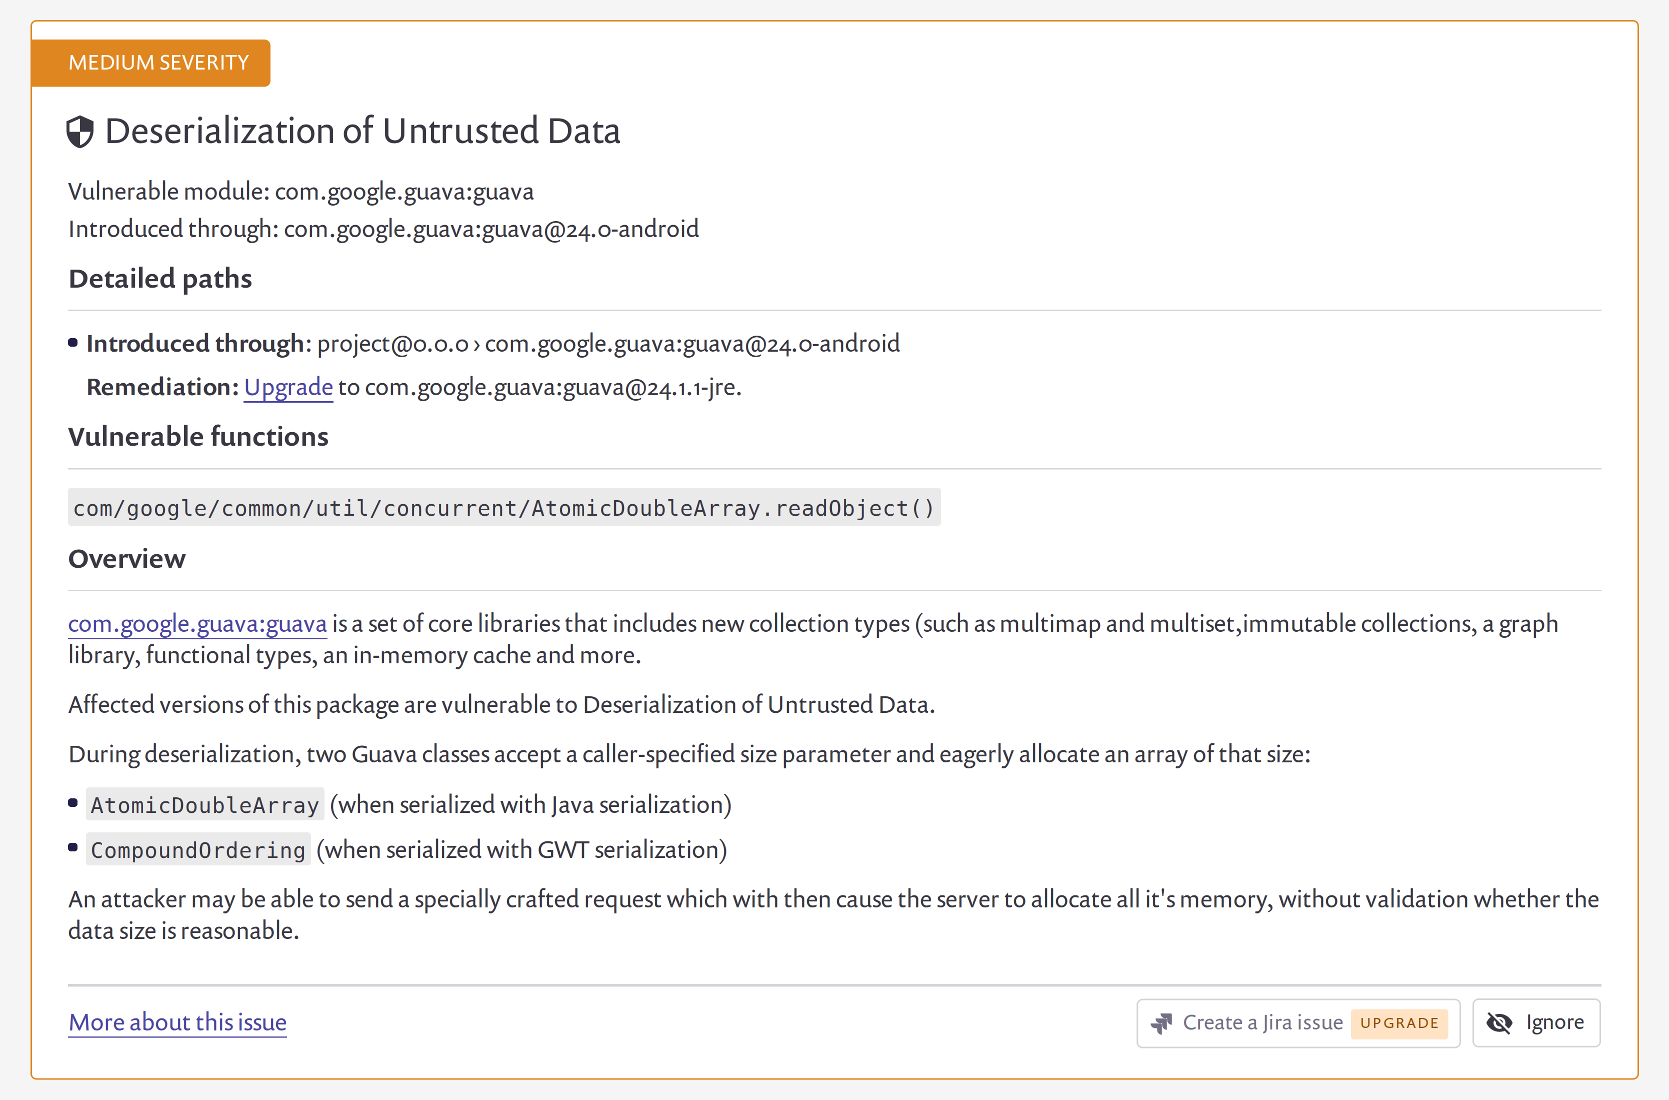
\includegraphics[width=0.9\linewidth]{snyk.png}\end{adjustbox}
    \end{MyMdframed}
\end{figure}

Snyk vulnerabilities relating to deserialisation tend to be raised in large volumes for each \emph{gadget} discovered in
a library.
The system gives no weight to whether the application deserialises user input, does so in an unsafe way which allows any
type to be used, or indeed does any deserialisation at all.
In \emph{My Warwick}'s case, no automatic deserialisation is present at all, and so the is completely unexploitable.
This problem is a consequence of Snyk only analysing dependencies and not performing static analysis on the codebase to
determine if the problem is relevant or not.

At the time of writing, the company has introduced ``runtime monitoring'' to determine if insecure functions are
actually called.
This functionality increases the value of the vulnerability reports, but only supports a limited number of platforms and
requires running an agent alongside the application to collect and send runtime data.

\chapter{Design}\label{ch:design}

This chapter discusses the design decisions made throughout the project and the reasoning behind them.

\section{Programming Language}
This section covers the design of the language's syntax, its type system, the foreign function interface (FFI) and
interpreter.

The need for our language to be predictable and familiar to developers is clear.
We therefore present an imperative proof-of-concept language, with a C-like syntax.
The aim is that developers, and particularly those that work with JVM technologies, will be able to write critical
sections of code within our language, where regex refinements are available.

At build time, the language tooling should progress through a series of stages:

\tikzstyle{line} = [draw, -latex']
\tikzset{arrow/.style={
minimum height=1.2cm,%
inner sep=1em,
shape=signal,
signal from=west,
signal to=east,
signal pointer angle=110,
text depth=.25ex,
text height=1.5ex,
fill=id7-aubergine,
baseline,
text centered, text=white
}}

\resizebox*{0.95\textwidth}{!}{\begin{tikzpicture}[node distance=-\pgflinewidth, auto, baseline={([yshift={-1.25ex}]current bounding box.center)}]
\sffamily{
\begin{scope}[start chain=transition going right,node distance=-\pgflinewidth]
\node [arrow, on chain] {\faStream{} Parsing};
\node [arrow, on chain] {\faChartNetwork{} AST Construction};

\node [arrow, on chain] {\faClipboardCheck{} Type checking};
\node [arrow, on chain] {\faFlag{} Reporting};
\node [arrow, on chain] {\faCogs{} Interpreting};
\end{scope}
}
\end{tikzpicture}}

We use this multi-stage process for a number of reasons:

\begin{itemize}
    \item Type checking requires more than one pass over the syntax tree.
          In particular, we allow \emph{forward references} to functions that appear later in the program source code.
          Whilst this flexibility is likely to be welcomed by e.g. Java developers who also enjoy this freedom,
          it requires that we process the parse tree in two phases in order to detect issues such as references to
          undefined functions.
    \item Code can be separated into smaller self-contained components for each of the distinct stages
          which can then be more effectively unit tested.
    \item Later stages can use a higher-level AST representation and need not be concerned with exact syntax or
          underlying code which the parser has already processed.
\end{itemize}


\subsection{Syntax}\label{subsec:syntax}

The C-like syntax, with some influence from other languages such as Go, is augmented with the use of square brackets
to specify refinement types.
This is inspired by languages such as Scala which use square brackets after types for parametric polymorphism,
e.g. \mintinline{scala}{val numbers: List[Int] = List(1, 2, 3)}.

Below, we show a high-level BNF grammar for our language.
This was constructed, made unambiguous and then used as a basis during the implementation phase.

\setlength{\grammarparsep}{20pt plus 1pt minus 1pt} % increase separation between rules
\setlength{\grammarindent}{12em} % increase separation between LHS/RHS

We begin by defining our main rule to represent a complete program.
Programs contain a number of functions, which are declared with an identifier, number of arguments and a return type.

\begin{grammar}
    <program> ::= (<function> \textbackslash n)*
    <function> ::= <function-signature> <body> `\}'

    <function-signature> ::= `function' ` ' <identifier> `(' <parameter-decl> `): ' <type> `\{\textbackslash n'

    <body> ::= (<body-line> \textbackslash n)*

    <parameter-decl> ::= <expr> `: ' <type>
    \alt <expr> `: ' <type> `, ' <parameter-decl>
    \alt <empty>
\end{grammar}

We can now start to define what is permitted inside the lines that sit within a function body.
We want to be able to declare local variables, assign values to them, call functions (discarding any return type) or
control the flow of execution using \emph{selection}.

\begin{grammar}
    <body-line> ::= <var-assignment>
        \alt <return-stmt>
        \alt <var-decl>
        \alt <function-call>
        \alt <if-stmt>

    <var-assignment> ::= <identifier> `=' <expr>

    <return-stmt> ::= `return' <expr>

    <var-decl> ::= `var' <identifier> `: ' <type>

    <function-call> ::= <identifier> `(' <argument-list> `)'

    <argument-list> ::= <expr> | <expr> `,' <argument-list>
    \alt <empty>
\end{grammar}

Selection in the language is implemented with an \textbf{if}-\textbf{else if}-\textbf{else} construct
as one might see in other imperative languages such as C.
Such a statement has no limit on the number of \textbf{else if} components.

Again, this is motivated by a desire for parity with other programming languages.

\begin{grammar}
    <if-stmt> ::= `if` ` ' `(' <expr> `)' ` ' `\{ \textbackslash n' <body> `\}' <optional-else>

    <optional-else> ::= ` ' `else' ` ' `\{ \textbackslash n' <body> `\}' \alt ` ' `else' ` ' if_stmt \alt <empty>

\end{grammar}

We now turn our attention to the type system, and support for refinements (encompassed in the \texttt{<constraint>} rule) in the grammar.
The language supports the following type keywords:

\arrayrulecolor{white}
\begin{table}[H]

    \centering
    \rowcolors{1}{id7-aubergine-tint}{lightgrey}
    \begin{tabular}[t]{|p{3cm}|p{8cm}|}
        \hline
        \rowcolor{id7-aubergine}
        {\color[HTML]{FFFFFF} \sffamily \textbf{Type Keyword}} & {\color[HTML]{FFFFFF} \sffamily \textbf{Description}} \\ \hline
        \texttt{string} & A collection of characters. May be refined to be a regular expression member. \\ \hline
        \texttt{uint} & An unsigned integer. May include a refinement to be greater/less than a threshold. \\ \hline
        \texttt{bool} & An ordinary Boolean value which may be \texttt{true} or \texttt{false}. No applicable refinements. \\ \hline
        \texttt{void} & Used for functions with no return type. \\ \hline
    \end{tabular}
\end{table}

As a proof of concept, this small set of types allows for small programs to be expressed whilst limiting the complexity
of the language to ensure it is tractable to implement.

We define the \texttt{<type>} class to represent a type reference.
This class is then used throughout the grammar for function parameter types, local variables types and return
types.

\begin{grammar}
    <type> ::= <type-keyword> | <type-keyword> `[' <constraint> `]'

    <type-keyword> ::= `void' | `uint' | `bool' | `string'

    <constraint> ::= `>' <number> \alt `<' <number> \alt `>=' <number> \alt `<=' <number> \alt `/' <re> `/'
\end{grammar}

Integer refinements are a relatively straightforward affair, as shown above.
The developer can restrict the domain of values to be greater-than or less-than a constant numeric literal.

We now parse regular expression refinements using the parsing hierarchy proposed in \citet{cameron1999}.
This hierarchy allows regular expressions to be processed in an intuitive manner with the Kleene star/plus operations
binding more strongly than concatenation and alternation:

\begin{description}
    \item[\texttt{aab*c}] Should be interpreted as \texttt{aa(b)*c}.
    \item[\texttt{ab|cd|ef}] Should be interpreted as \texttt{(ab)|(bc)|(cd)}.
\end{description}

We amend the production rules used by \citeauthor{cameron1999} to ensure they are unambiguous, by creating
prime-suffixed classes with $\epsilon$-productions.

\label{regex:parse}

\begin{grammar}

    <re> ::= <simple-re> <union-prime>

    <union-prime> ::= `|' <re> | <empty>

    <simple-re> ::= <basic-re> <concat-prime>

    <concat-prime> ::= <simple-re> | <empty>

    <basic-re> ::= <kleene-star> | <plus> | <elementary-re>

    <kleene-star> ::= <elementary-re> `*'

    <plus> ::= <elementary-re> `+'

    <elementary-re> ::= <group> | `.' | <character> | <range-re>

    <group> ::= `(' re `)'

    <range-re> ::= <positive-range> | <negated-range>

    <positive-range> ::= `[' <range-items> `]'

    <negated-range> ::= `[^' <range-items> `]'

    <range-items> ::= <range-item> | <range-item> <range-items>

    <range-item> ::= <character> `-' <character> | <character>

\end{grammar}

A sample parse tree for the regular expression \texttt{[A-Z]+a} is given in figure \ref{fig:regex:parsetree}.

\begin{figure}
\begin{MyMdframed}
\vspace{0.5em}

\caption{\label{fig:regex:parsetree}Result of parsing using \citeauthor{cameron1999}'s amended hierarchy for the expression \texttt{[A-Z]+a}}
\vspace{0.5em}
\captionsetup{style=default}
 \begin{center}
    \begin{forest}
[re
  [simple\_re
    [basic\_re
      [plus
        [elementary\_re
          [range
            [positive\_range
              [{[}]
[range\_items
                [range\_item
                  [lax\_character
                    [A]
                    ]
[-]
[lax\_character
                    [Z]
                    ]
                  ]
                ]
[{]}]
              ]
            ]
          ]
[+]
        ]
      ]
[concat\_prime
      [simple\_re
        [basic\_re
          [elementary\_re
            [character
              [a]
              ]
            ]
          ]
[concat\_prime]
        ]
      ]
    ]
[union\_prime]
  ]
[/]
]
[{]}]
]]
    \end{forest}
  \end{center}
\end{MyMdframed}
\end{figure}

We define expressions to permit basic arithmetic operations, nesting and function calls:

\begin{grammar}
<expr> ::= <expr> (`*'|`/') <expr>
    \alt <expr> (`+'|`-') <expr>
    \alt <value_ref>
    \alt <expr> ` ' (`<'|`>'|`<='|`>='|`==') ` ' <expr>
    \alt <function-call>
    \alt <value-ref>

<value-ref> ::= <number> | <string-literal> | `true' | `false' | <identifier>
\end{grammar}

Finally, we set-up the most basic rules for setting what is permitted as an identifier name, string literal or
number:

\begin{grammar}
    <number> :== <digit> | <integer> <digit>

    <digit> :== `0' | `1' | `2' | `3' | `4' | `5' | `6' | `7' | `8' | `9'

    <string-literal> :== `\textquotedbl{}' (<character> *) `\textquotedbl{}'

    <identifier> :== <alpha> (<alphanumeric> *)
\end{grammar}

The result is a small imperative language which can be used to implement simple logic.
Code can be reused by way of user-defined functions.
Included below are some illustrative examples of basic programs written in the discussed syntax:

\begin{mycodefile}{rrtlex.py:RrtLexer -x}{\label{code:rrt:1}A factorial function written in the RRT language}{RRT}{factorial.rrt}
    \vspace{0.5em}

    In this example, we use the unrefined \texttt{uint} type to implement the factorial function, where
    $5! = 5\times 4 \times 3 \times 2 \times 1$.
\end{mycodefile}

We can also begin to use refinement types in our program code:

\begin{mycodefile}{rrtlex.py:RrtLexer -x}{\label{code:rrt:2}A product function, which multiplies its arguments}{RRT}{integer-refinements.rrt}
    \vspace{0.5em}

    Here, we use integer refinement types to restrict the domain of the arguments to the \texttt{Product}
    function.
    The first number, \texttt{a}, is required to be less than 10 whereas \texttt{b} must be less than or equal to 15.
\end{mycodefile}

\label{sec:grammar}

\subsection{Abstract Syntax Tree}

Combined with a parser generator, the grammar discussed in section \ref{sec:grammar} enables programs to be parsed into
a data structure known as a \emph{Concrete Syntax Tree} (CST) which maps directly to the grammar.

Whilst the CST is useful, most type checking will require a richer representation of a program written in our language.
For example, the current grammar would parse refinements such as \textcolor{id7-ruby-red}{\texttt{uint}}\texttt{[/.*/]},
To check for these issues and interpret code, we use an \emph{Abstract Syntax Tree} (AST) representation of the program.

Unlike some (generally more functional languages), we make a distinction between \textit{statements} and
\textit{expressions}.
The former do not necessarily yield a value in the same way as expressions.
For example, an if statement may not return a value--it could simply call a function and rely on its side effects.
We make no claim that such a language is more elegant than others, but adoption is necessary for security tooling
to be effective; designing an imperative language which would be comfortable to e.g. Java developers was important,
since they are responsible for a great proportion of production code.

We rely on the object-oriented concept of inheritance when modelling our AST entities.
Expressions and statements can inherit from a common abstract base class and reuse their logic.

We first discuss the different types of expressions in our AST representation.
There are 9 of these.
We make a distinction between ``value'' expressions, where a value can be derived immediately, and those which require
computation to derive a value (e.g. a function call or arithmetic operation).

The diagram below show how the different expression types relate to each other:

\begin{figure}[H]
    \begin{MyMdframed}
        \vspace{0.5em}

        \caption{\label{figure:ast:expressions}Expression AST objects}
        \vspace{0.5em}
        \captionsetup{style=default}

        \centering 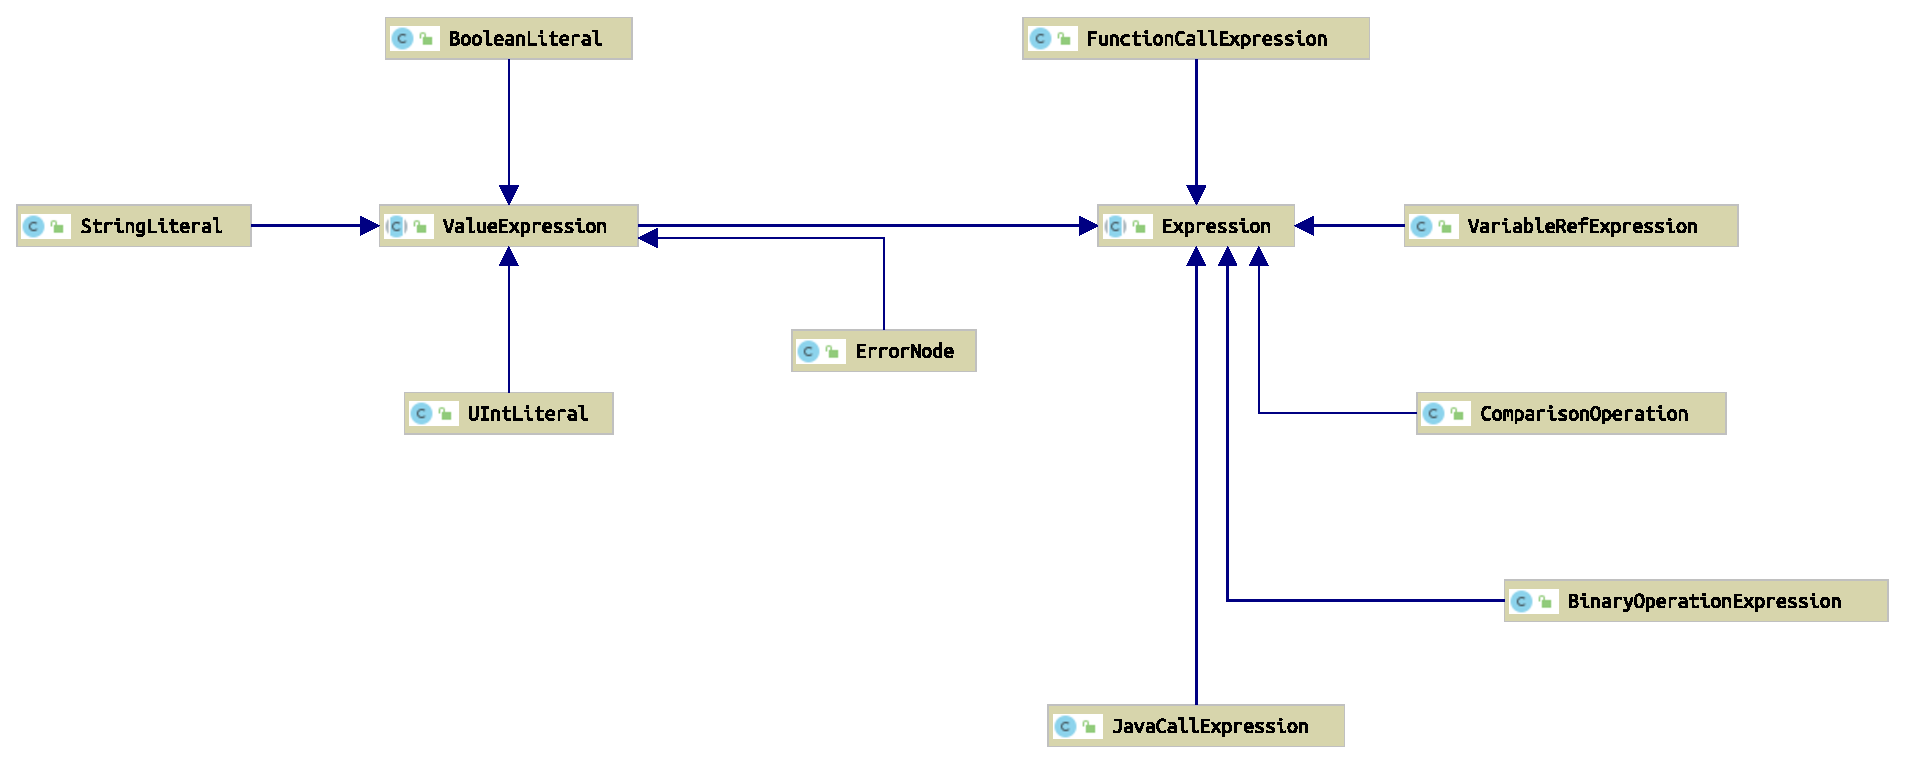
\includegraphics[width=0.9\linewidth]{expressions.eps}
    \end{MyMdframed}
\end{figure}

\begin{description}
    \item[JavaCallExpression] Models a expression which involves a foreign function interface call to a static JVM class method.
    \item[BinaryOperationExpression] Represents an expression involving a binary operation, and two child nodes to which the operation is applied.
    \item[ValueExpression] Parent object for value expressions, as discussed above.
    \item[FunctionCallExpression] Represents a call to a non-void function, where the return value is used.
    \item[VariableRefExpression] Encapsulates a reference to another variable which is in scope (either a function parameter or local variable).
    \item[Expression] Parent of all expressions, defines operations to evaluate their value for use by the interpreter.
    \item[StringLiteral] Represents a string literal defined in code, such as  \mintinline{rrtlex.py:RrtLexer -x}{"Hello, world"}.
    \item[UIntLiteral] Represents an unsigned integer literal defined in code, such as  \mintinline{rrtlex.py:RrtLexer -x}{6}.
    \item[BooleanLiteral] Represents a boolean literal--\mintinline{rrtlex.py:RrtLexer -x}{true} or \mintinline{rrtlex.py:RrtLexer -x}{false}.
\end{description}

All expression types must provide a way for the expression to be evaluated (yielding a value).

The diagram below shows the structure of our statement-related entities:

\begin{figure}[H]
    \begin{MyMdframed}
        \vspace{0.5em}

        \caption{\label{figure:ast:statements}Statement AST objects}
        \vspace{0.5em}
        \captionsetup{style=default}

        \centering 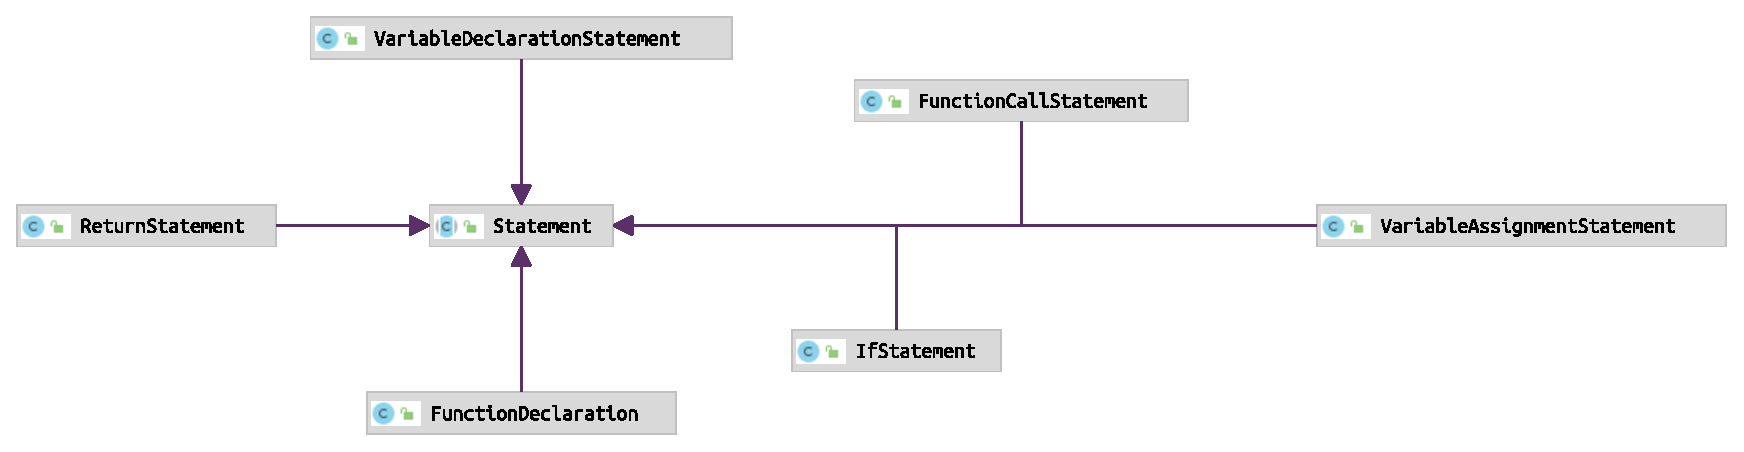
\includegraphics[width=0.9\linewidth]{statements.eps}
    \end{MyMdframed}
\end{figure}

\begin{description}
    \item[VariableDeclarationStatement] Models a statement of type \mintinline{rrtlex.py:RrtLexer -x}{var variable: string[/A+/]}.
    \item[FunctionCallStatement] Models a statement of type \mintinline{rrtlex.py:RrtLexer -x}{Function()}, where the return value is unused.
    \item[VariableAssignmentStatement] Handles assignment of a value to a variable, \mintinline{rrtlex.py:RrtLexer -x}{variable="AAA"}
    \item[IfStatement] Represents a control flow statement comprising an \textbf{\textcolor{id7-aubergine}{\texttt{if}}} clause and one or more \textbf{\textcolor{id7-aubergine}{\texttt{else}}}/\textbf{\textcolor{id7-aubergine}{\texttt{else if}}} clauses.
    \item[FunctionDeclaration] Encapsulates data relating to a function such as the parameters it takes, an identifier and its return type.
    \item[ReturnStatement] Represents a line in a function body which returns a value, e.g. \mintinline{rrtlex.py:RrtLexer -x}{return 6}.
\end{description}

Each statement is endowed with an \texttt{execute} operation which can optionally return a value in the form of an
expression.

Entities encapsulate data according to their purpose.
An \textit{IfStatement} object contains an expression that is evaluated to produce a Boolean value, a reference to the
bodies of code to execute if the expression is true (or false) and a reference to a further \textit{IfStatement} if an
\mintinline{rrtlex.py:RrtLexer -x}{else if} is present.

\subsection{Type System}

In some languages, such as JavaScript, the type system can be described as `weak'.
Types can be used in different contexts and will be \emph{coerced} as necessary.
For example, it is possible to ``add'' unrelated objects, resulting in a conversion to two strings which are then
concatenated:

\termbox{
\texttt{\textcolor{term-green}{\fallbackmono{➜}} \ttfamily \textbf{\textcolor{term-dir}{\textasciitilde} node}}\\
\texttt{> String([])}\\
\textcolor{term-green}{\texttt{''}}\\
\texttt{> String({})}\\
\textcolor{term-green}{\texttt{'[object Object]'}}\\
\texttt{> []+{}}\\
\textcolor{term-green}{\texttt{'[object Object]'}}\\
}

In the above REPL (read-eval-print loop) session, use of the \texttt{+} operator automatically coerces the operands
into their string representation and then concatenates them together.
This behaviour is characteristic of a weakly-typed language, and is not particularly intuitive.
Furthermore, it can lead to problems which are only observed once a system has been deployed into production.

Our language type system is \emph{strongly} and \emph{statically} typed.


Types need to be checked in a number of situations:

\begin{itemize}
    \item New value is assigned to a local variable
    \item Value is passed to a function as an argument
    \item Value is returned from a function
\end{itemize}

For simple types with no refinements, this is generally a straightforward check.
As our language is strongly typed, we simply need to check that the expected and actual types are an exact match.
No implicit conversions are supported in our language.

Refined types are more involved: it is not enough for us to check that the refinements are the same.
Observe that a variable of type \texttt{uint[< 10]} is perfectly valid to return from a function with a return type of
\texttt{uint[<= 20]}.
We must instead determine if the refinement types are \emph{compatible}.
We define two refinement types $\tau_e, \tau_a$ (expected and actual) to be compatible if there is no value $v:~\tau_a$
in the actual type that is not in $\tau_e$ and is therefore in the complement of the expected type $(\tau_e)^C$.

A concrete example involving integer refinements is given below:

\begin{mycodefile}{rrtlex.py:RrtLexer -x}{foo}{RRT}{irt.rrt}\end{mycodefile}

In the above listing, we need to compare types on 2 occasions:

\begin{enumerate}
    \item When $6$ is assigned to $x$ (to check it is greater than $5$)
    \item When $x$ is returned from the function \texttt{Demonstration} (to check $> 5$ is compatible with $> 10$)
\end{enumerate}

The first check is trivially accomplished because there are no unknowns.
The second check can be expressed in CNF as an SMT formula, using the complement as discussed: $x > 5 \land x <= 10$.

This problem can be checked using DPLL(T) as described in section \ref{dpllt}.
We formulate a SAT problem $A \land B$, receive a satisfying valuation $\{A=T, B=T\}$ and pass this to the theory
solver.
As the reader will appreciate, it is then trivial to satisfy this formula with any value between $6$ and $10$.
Hence, we have found a violation and the types are incompatible.

The language type checker implements exactly this process.
Constraints are built based on the types identified during AST construction and then solved using an SMT solver.
With a theory solver available for both integers and strings, this approach works for both kinds of refinements
supported by the language.

\section{Foreign Function Interface}

For interoperability with existing JVM code, we devised a mechanism whereby developers could call arbitrary JVM
code in the presence of some satisfied pre-conditions.
This foreign function interface is designed to allow:

\begin{itemize}
    \item Calling of arbitrary static Java methods
    \item Passing of first-class types from within the language to the Java method, provided they can be converted
    \item Use of the return value from the Java method, provided it can be converted into an appropriate type
\end{itemize}

We only consider static methods because the proof-of-concept language does not support any object-oriented
programming features and so instantiating an object to call an instance method would not be feasible.

Foreign calls should be treated like all other expressions in the language, allowing the return value of these
methods to be assigned to local variables, returned or otherwise manipulated.


\section{Development Methodology}

It is important, for any project with significant elements of software engineering, that development is approached in a
way which enables any changes to system requirements to be handled quickly.

For this project, we used a number of features of agile software development methodologies such as Scrum to plan development work.
The Scrum methodology involves ``sprints'' which are a fixed duration and planned in advance based on tasks in the backlog \citep{sutherland2014scrum}.

We scheduled a series of one-week sprints to implement the functionality discussed throughout this chapter.
This approach allows for progress to be reflected upon at the end of each sprint.

\chapter{Implementation}

\section{Parsing}

\subsection{Introduction}

In order to lex and parse user input into the AST structure discussed earlier, we use the \emph{ANTLR4} parser generator.
ANTLR4 generates $LL(*)$ parsers in a variety of languages, including Java, C\# and Go \citep{parr2011ll}.
These parsers are not restricted to a fixed number of lookahead tokens.
ANTLR instead generates a series of \emph{lookahead DFAs} which help the parser to make decisions based on whether
successive tokens belong to a regular language or not (in which case, backtracking begins) \citep[p.~3]{parr2011ll}.

The grammar is split into two distinct files.
One file defines the rules for the lexer, which is responsible for tokenising the source code.
The second file describes the parser which ANTLR will generate.
The parsing rules generally resemble the BNF discussed previously in section \ref{subsec:syntax}, so we will not
dwell on them here.
The lexer is more involved than a simple translation from BNF, because the language syntax requires that we make use of
\emph{lexical states}.

Consider the token definitions for variable/function identifiers and characters that can appear in a regular expression:

\begin{minted}{antlr}
IDENTIFIER : [A-Za-z_] [A-Za-z_0-9]* ;
CHARACTER  : ~('\n'|'\r'|'.'|'('|')'|'['|']'|'*'|'+'|'/'|'|') | ESCAPED_META;
\end{minted}

As the two token definitions overlap, they cannot appear in use together in the same lexical state.
If they did, only one would be identified by the lexer, breaking the parsing of either the regular expressions, or the
function definitions.

To solve this, we define two new lexical states using the \textbf{\texttt{mode}} keyword:

\newsavebox\myvlex

\begin{lrbox}{\myvlex}\begin{minipage}{\textwidth}
  \begin{mycodefile}{antlr}{\label{code:antlr:1}Using lexical states in the lexer}{ANTLR}{antlrlex.g4}
  \end{mycodefile}
\end{minipage}\end{lrbox}

\begin{Verbatim}[commandchars=\\\{\}]
\PYGidseven{k}{lexer}\PYGidseven{+w}{ }\PYGidseven{k}{grammar}\PYGidseven{+w}{ }\PYGidseven{n+nl}{PocLex}\PYGidseven{+w}{ }\PYGidseven{p}{;}
\PYGidseven{k}{mode}\PYGidseven{+w}{ }\PYGidseven{n+nl}{REGEX;}
\PYGidseven{n+nl}{BEGIN\PYGidsevenZus{}RE\PYGidsevenZus{}RANGE}\PYGidseven{+w}{ }\PYGidseven{p}{:}\PYGidseven{+w}{ }\PYGidseven{l+s}{\PYGidsevenZsq{}[\PYGidsevenZsq{}}\PYGidseven{+w}{ }\PYGidseven{o}{\PYGidsevenZhy{}\PYGidsevenZgt{}}\PYGidseven{+w}{ }\PYGidseven{n+nv}{pushMode}\PYGidseven{o}{(}\PYGidseven{n+no}{REGEX\PYGidsevenZus{}RANGE}\PYGidseven{o}{)}\PYGidseven{+w}{ }\PYGidseven{p}{;}
\PYGidseven{n+nl}{END\PYGidsevenZus{}RE\PYGidsevenZus{}RANGE}\PYGidseven{+w}{   }\PYGidseven{p}{:}\PYGidseven{+w}{ }\PYGidseven{l+s}{\PYGidsevenZsq{}]\PYGidsevenZsq{}}\PYGidseven{+w}{ }\PYGidseven{p}{;}
\PYGidseven{n+nl}{CHARACTER}\PYGidseven{+w}{      }\PYGidseven{p}{:}\PYGidseven{+w}{ }\PYGidseven{o}{\PYGidsevenZti{}(}\PYGidseven{l+s}{\PYGidsevenZsq{}\PYGidsevenZbs{}n\PYGidsevenZsq{}}\PYGidseven{o}{|}\PYGidseven{l+s}{\PYGidsevenZsq{}\PYGidsevenZbs{}r\PYGidsevenZsq{}}\PYGidseven{o}{|}\PYGidseven{l+s}{\PYGidsevenZsq{}.\PYGidsevenZsq{}}\PYGidseven{o}{|}\PYGidseven{l+s}{\PYGidsevenZsq{}(\PYGidsevenZsq{}}\PYGidseven{o}{|}\PYGidseven{l+s}{\PYGidsevenZsq{})\PYGidsevenZsq{}}\PYGidseven{o}{|}\PYGidseven{l+s}{\PYGidsevenZsq{}[\PYGidsevenZsq{}}\PYGidseven{o}{|}\PYGidseven{l+s}{\PYGidsevenZsq{}]\PYGidsevenZsq{}}\PYGidseven{o}{|}\PYGidseven{l+s}{\PYGidsevenZsq{}*\PYGidsevenZsq{}}\PYGidseven{o}{|}\PYGidseven{l+s}{\PYGidsevenZsq{}+\PYGidsevenZsq{}}\PYGidseven{o}{|}\PYGidseven{l+s}{\PYGidsevenZsq{}/\PYGidsevenZsq{}}\PYGidseven{o}{|}\PYGidseven{l+s}{\PYGidsevenZsq{}|\PYGidsevenZsq{}}\PYGidseven{o}{)}\PYGidseven{+w}{ }\PYGidseven{o}{|}\PYGidseven{+w}{ }\PYGidseven{n+no}{ESCAPED\PYGidsevenZus{}META}\PYGidseven{p}{;}
\PYGidseven{n+nl}{BEGIN\PYGidsevenZus{}RE\PYGidsevenZus{}GROUP}\PYGidseven{+w}{ }\PYGidseven{p}{:}\PYGidseven{+w}{ }\PYGidseven{l+s}{\PYGidsevenZsq{}(\PYGidsevenZsq{}}\PYGidseven{+w}{ }\PYGidseven{p}{;}
\PYGidseven{n+nl}{END\PYGidsevenZus{}RE\PYGidsevenZus{}GROUP}\PYGidseven{+w}{   }\PYGidseven{p}{:}\PYGidseven{+w}{ }\PYGidseven{l+s}{\PYGidsevenZsq{})\PYGidsevenZsq{}}\PYGidseven{+w}{ }\PYGidseven{p}{;}
\PYGidseven{n+nl}{MINUS}\PYGidseven{+w}{          }\PYGidseven{p}{:}\PYGidseven{+w}{ }\PYGidseven{l+s}{\PYGidsevenZsq{}\PYGidsevenZhy{}\PYGidsevenZsq{}}\PYGidseven{+w}{ }\PYGidseven{p}{;}
\PYGidseven{n+nl}{DOT}\PYGidseven{+w}{            }\PYGidseven{p}{:}\PYGidseven{+w}{ }\PYGidseven{l+s}{\PYGidsevenZsq{}.\PYGidsevenZsq{}}\PYGidseven{+w}{ }\PYGidseven{p}{;}
\PYGidseven{n+nl}{STAR}\PYGidseven{+w}{           }\PYGidseven{p}{:}\PYGidseven{+w}{ }\PYGidseven{l+s}{\PYGidsevenZsq{}*\PYGidsevenZsq{}}\PYGidseven{+w}{ }\PYGidseven{p}{;}
\PYGidseven{n+nl}{PLUS}\PYGidseven{+w}{           }\PYGidseven{p}{:}\PYGidseven{+w}{ }\PYGidseven{l+s}{\PYGidsevenZsq{}+\PYGidsevenZsq{}}\PYGidseven{+w}{ }\PYGidseven{p}{;}
\PYGidseven{n+nl}{ALTERNATION}\PYGidseven{+w}{    }\PYGidseven{p}{:}\PYGidseven{+w}{ }\PYGidseven{l+s}{\PYGidsevenZsq{}|\PYGidsevenZsq{}}\PYGidseven{+w}{ }\PYGidseven{p}{;}
\PYGidseven{n+nl}{RANGE\PYGidsevenZus{}NEGATE}\PYGidseven{+w}{   }\PYGidseven{p}{:}\PYGidseven{+w}{ }\PYGidseven{l+s}{\PYGidsevenZsq{}\PYGidsevenZca{}\PYGidsevenZsq{}}\PYGidseven{+w}{ }\PYGidseven{p}{;}
\PYGidseven{n+nl}{RE\PYGidsevenZus{}DELIMITER\PYGidsevenZus{}CLOSE}\PYGidseven{p}{:}\PYGidseven{+w}{ }\PYGidseven{l+s}{\PYGidsevenZsq{}/\PYGidsevenZsq{}}\PYGidseven{+w}{ }\PYGidseven{o}{\PYGidsevenZhy{}\PYGidsevenZgt{}}\PYGidseven{+w}{ }\PYGidseven{n+nv}{popMode}\PYGidseven{+w}{ }\PYGidseven{p}{;}
\PYGidseven{n+nl}{META\PYGidsevenZus{}CHAR}\PYGidseven{+w}{      }\PYGidseven{p}{:}\PYGidseven{+w}{ }\PYGidseven{o}{(}\PYGidseven{n+no}{DOT}\PYGidseven{o}{|}\PYGidseven{n+no}{PLUS}\PYGidseven{o}{|}\PYGidseven{n+no}{STAR}\PYGidseven{o}{|}\PYGidseven{n+no}{ALTERNATION}\PYGidseven{o}{|}\PYGidseven{l+s}{\PYGidsevenZsq{}[\PYGidsevenZsq{}}\PYGidseven{o}{|}\PYGidseven{l+s}{\PYGidsevenZsq{}]\PYGidsevenZsq{}}\PYGidseven{o}{|}\PYGidseven{l+s}{\PYGidsevenZsq{}/\PYGidsevenZsq{}}\PYGidseven{o}{)}\PYGidseven{+w}{ }\PYGidseven{p}{;}
\PYGidseven{k}{fragment}\PYGidseven{+w}{ }\PYGidseven{n+nl}{ESCAPED\PYGidsevenZus{}FWD\PYGidsevenZus{}SLASH}\PYGidseven{p}{:}\PYGidseven{+w}{ }\PYGidseven{l+s}{\PYGidsevenZsq{}\PYGidsevenZbs{}\PYGidsevenZbs{}/\PYGidsevenZsq{}}\PYGidseven{+w}{ }\PYGidseven{p}{;}
\PYGidseven{k}{fragment}\PYGidseven{+w}{ }\PYGidseven{n+nl}{ESCAPED\PYGidsevenZus{}META}\PYGidseven{p}{:}\PYGidseven{+w}{ }\PYGidseven{l+s}{\PYGidsevenZsq{}\PYGidsevenZbs{}\PYGidsevenZbs{}\PYGidsevenZsq{}}\PYGidseven{+w}{ }\PYGidseven{n+no}{META\PYGidsevenZus{}CHAR}\PYGidseven{+w}{ }\PYGidseven{p}{;}

\PYGidseven{k}{mode}\PYGidseven{+w}{ }\PYGidseven{n+nl}{CONSTRAINT;}
\PYGidseven{n+nl}{GT}\PYGidseven{p}{:}\PYGidseven{+w}{ }\PYGidseven{l+s}{\PYGidsevenZsq{}\PYGidsevenZgt{}\PYGidsevenZsq{}}\PYGidseven{+w}{ }\PYGidseven{p}{;}
\PYGidseven{n+nl}{GE}\PYGidseven{p}{:}\PYGidseven{+w}{ }\PYGidseven{l+s}{\PYGidsevenZsq{}\PYGidsevenZgt{}=\PYGidsevenZsq{}}\PYGidseven{+w}{ }\PYGidseven{p}{;}
\PYGidseven{n+nl}{LT}\PYGidseven{p}{:}\PYGidseven{+w}{ }\PYGidseven{l+s}{\PYGidsevenZsq{}\PYGidsevenZlt{}\PYGidsevenZsq{}}\PYGidseven{+w}{ }\PYGidseven{p}{;}
\PYGidseven{n+nl}{LE}\PYGidseven{p}{:}\PYGidseven{+w}{ }\PYGidseven{l+s}{\PYGidsevenZsq{}\PYGidsevenZlt{}=\PYGidsevenZsq{}}\PYGidseven{+w}{ }\PYGidseven{p}{;}
\PYGidseven{n+nl}{EQ}\PYGidseven{p}{:}\PYGidseven{+w}{ }\PYGidseven{l+s}{\PYGidsevenZsq{}=\PYGidsevenZsq{}}\PYGidseven{+w}{ }\PYGidseven{p}{;}
\PYGidseven{n+nl}{CONSTRAINT\PYGidsevenZus{}UINT}\PYGidseven{p}{:}\PYGidseven{+w}{ }\PYGidseven{p}{[}\PYGidseven{x}{0\PYGidsevenZhy{}9}\PYGidseven{p}{]}\PYGidseven{o}{+}\PYGidseven{+w}{ }\PYGidseven{p}{;}
\PYGidseven{n+nl}{CONSTRAINT\PYGidsevenZus{}SPACE}\PYGidseven{p}{:}\PYGidseven{+w}{ }\PYGidseven{l+s}{\PYGidsevenZsq{} \PYGidsevenZsq{}}\PYGidseven{+w}{ }\PYGidseven{p}{;}
\PYGidseven{n+nl}{RE\PYGidsevenZus{}DELIMITER\PYGidsevenZus{}OPEN}\PYGidseven{p}{:}\PYGidseven{+w}{ }\PYGidseven{l+s}{\PYGidsevenZsq{}/\PYGidsevenZsq{}}\PYGidseven{+w}{ }\PYGidseven{o}{\PYGidsevenZhy{}\PYGidsevenZgt{}}\PYGidseven{+w}{ }\PYGidseven{n+nv}{pushMode}\PYGidseven{o}{(}\PYGidseven{n+no}{REGEX}\PYGidseven{o}{)}\PYGidseven{+w}{ }\PYGidseven{p}{;}
\PYGidseven{n+nl}{END\PYGidsevenZus{}CONSTRAINT}\PYGidseven{+w}{   }\PYGidseven{p}{:}\PYGidseven{+w}{ }\PYGidseven{l+s}{\PYGidsevenZsq{}]\PYGidsevenZsq{}}\PYGidseven{+w}{ }\PYGidseven{o}{\PYGidsevenZhy{}\PYGidsevenZgt{}}\PYGidseven{+w}{ }\PYGidseven{n+nv}{popMode}\PYGidseven{+w}{ }\PYGidseven{p}{;}
\end{Verbatim}



When the lexer identifies characters which begin constraints after a type keyword, it is directed to enter the
\texttt{CONSTRAINT} state.
From here, the forward slash regular expression delimiter prompts the lexer to enter the \texttt{REGEX} state where
regular expressions are tokenised.
States are maintained in a manner not dissimilar to a call stack.
If this delimiter is not observed, integer constraints can be tokenised instead.

Once the lexer reaches the end of an expression, it pops back into the previous lexical state and continues parsing.

\subsection{Working with ANTLR}

Once the grammar files are complete, ANTLR can be configured to generate parsers for a variety of languages.
We decided to implement the type checker and interpreter in Java, so we target Java for the generated parser.

Using the \emph{Gradle} build system, there is an official \texttt{antlr} plugin which provides a
\texttt{generateGrammarSource} build task.
When the grammar is modified, Gradle will regenerate the parser and lexer before compiling the rest of the Java
code within the project.

Following parser and lexer generation, it is straightforward to use them to process user input:

\begin{mycodefile}{java}{\label{code:antlr:2}Using ANTLR's lexing and parsing APIs}{Java}{antlruse.java}
    \vspace{0.5em}

    Implementing the \emph{visitor} pattern \citep{gof1995}, we can then process the concrete syntax tree which ANTLR
    has generated by parsing the program.
    \vspace{0.5em}

    \begin{minted}{java}
public class VisitorListener extends PocLangBaseListener {

    @Override
    public void enterProgram(PocLang.ProgramContext ctx) {
        // called when program non-terminal begins
    }
}
    \end{minted}
    Various methods can be defined on the listener and will be triggered when the nodes of a given type are encountered
    in the tree.
\end{mycodefile}

ANTLR can also be configured to target other languages, such as Go.
This is significant, because Go supports compiling to \emph{WebAssembly} which most modern browsers can run natively,
client-side.

\section{SMT Solvers}

Initially, our type checker made use of the JavaSMT abstraction layer to implement a subset of the language
supporting natural number refinements only.
This library provides a common API which is agnostic as to the underlying SMT solver.
This approach allows type incompatibilities to be discovered for refined unsigned integers.

The code below shows how the API can be used to set-up a small problem, determine if it is satisfiable, and print
the satisfying valuation/model for the variables in the problem:

\begin{mycodefile}{java}{Using the JavaSMT API}{Java}{javasmt.java}\end{mycodefile}

Once the initial prototype for a language with refinement types for natural numbers was completed and a set of passing
test cases had been written, the focus shifted to adding \texttt{string} support.

Unfortunately, string (and regular expression support) is not universal amongst SMT solvers--and JavaSMT did not
provide an abstraction layer over such functionality.

Thus, we needed to build Z3 from source and use its Java bindings instead of the JavaSMT library.
Z3, a C++ SMT solver, includes the Z3str3 component which is able to efficiently support solving string equations
and predicates involving regular language membership \citep{berzish2017z3str3}.
The original code which used the JavaSMT APIs to solve constraint problems with integers was then modified to use Z3.
An adapter was written to construct a Z3 regular expression object from the parse tree.

Z3's API is reasonably straight-forward to use from Java.
The example below shows what is involved in formulating and solving string constraint problems:

We first must build the regular expressions which we want to use as constraints.
In the same way that regular expressions can be defined inductively, Z3 offers an API that allows us to build up complex
\texttt{ReExpr} objects by repeatedly applying operations to them:

\begin{minted}{java}
// /[a-z!]+/
ReExpr matchAnyChar = ctx.mkPlus(
    ctx.mkUnion(
        ctx.mkRange(ctx.mkString("a"), ctx.mkString("z")), // [a-z]
        ctx.mkToRe(ctx.mkString("!")) // !
    )
);

// /foo[a-z!]+/, uses result above
ReExpr exprOne = ctx.mkConcat(ctx.mkToRe(ctx.mkString("foo")), matchAnyChar);
// /[a-z!]+bar/
ReExpr exprTwo = ctx.mkConcat(matchAnyChar, ctx.mkToRe(ctx.mkString("bar")));
\end{minted}

With our regular expression objects built, we can now create the string equation.
This requires an unknown variable $x$ of string type (or ``sort'' in Z3 parlance) and a \texttt{Solver} instance,
which we can inform of our constraints.

\begin{minted}{java}
// our unknown string, denoted by x
SeqExpr x = (SeqExpr) ctx.mkConst(ctx.mkSymbol("x"), ctx.getStringSort());

// make a new solver
Solver s = ctx.mkSolver();

// must satisfy both expressions - x must belong to the intersection
s.add(ctx.mkInRe(x, ctx.mkIntersect(exprOne, exprTwo)));
\end{minted}

With the constraints in place, we can begin searching for a satisfying model.
Z3 will try to find a string for $x$ which matches both expressions:

\begin{minted}{java}
// try and find model satisfying requirements
Status res = s.check();

// prints SATISFIABLE in this case
// but could print UNKNOWN, or UNSATISFIABLE
System.out.println(res);
// print out value from the model, e.g. "fooc!bar"
System.out.println(s.getModel().getConstInterp(x));
\end{minted}

When regular expression refinement types are encountered, the aforementioned adapter is used to build a Z3 compatible
\texttt{ReExpr} object from the parse tree discussed in the design section \ref{regex:parse}.
For string literals in the program code, these are represented by the regular expression that matches only the string
within the literal.

\section{Integrations and Frontends}

In this section, we present the various tools and integrations we have provide on top of the core parser, type checker
and interpreter.

\subsection{Command Line Interface}

We built a basic command line interface which would read programs from the standard input (stdin) stream.
Program text would be passed to the lexer, parser and then type checked.

Example output is shown below:

\termbox{
    \texttt{\textcolor{term-green}{\fallbackmono{➜}} \ttfamily \textbf{\textcolor{term-dir}{PocLang} \textcolor{term-git}{(git:}\textcolor{term-branch}{master}\textcolor{term-git}{)}} cat input.txt | ./gradlew run}\\
    \texttt{\textbf{> Task :run}}\\
    \textcolor{term-green}{\texttt{Reading program from stdin (use Ctrl+D when finished)...}}\\
    \textcolor{id7-ruby-red}{\texttt{Violation via value "gggg"}}\\
    \textcolor{id7-ruby-red}{\texttt{L5:4 Return type string [/g+|f+/] of function SecondaryFunction didn't satisfy string [/f+/], example violating value: "gggg"}}
}

This interface was useful during development, when implementing the type checker was the priority and the usability
of the interface was not as much of a consideration.

However, it is difficult to edit programs entered at the command line.
This made the interface impractical for experimenting in order to learn and explore the language.
No syntax highlighting could be provided, and line references had to be manually matched up to determine where
issues arose in the input.

\subsection{Web Application Interface}

Due to the limitations discussed with the command line interface, we also built a graphical web interface.
A screenshot is included overleaf.

As illustrated, users can enter code into the application.
We use a WebAssembly program, compiled from Go and using the same ANTLR lexer, to parse the program in real-time in
the browser.
This allows us to provide syntax recognition and highlighting which is identical in implementation to the Java backend.

When the user clicks the ``Perform type checks'' button, the program is sent to the backend Java type-checker application
which runs a HTTP server.
This server uses the same API as the original command line interface, but returns data in the JSON interchange format.
The browser then uses this type checking data to display annotations directly on the relevant line(s) indicating to the
user where type violations have occurred.

The following sequence diagram sketch illustrates the steps involved in the process, and each component's
responsibility:

\begin{center}
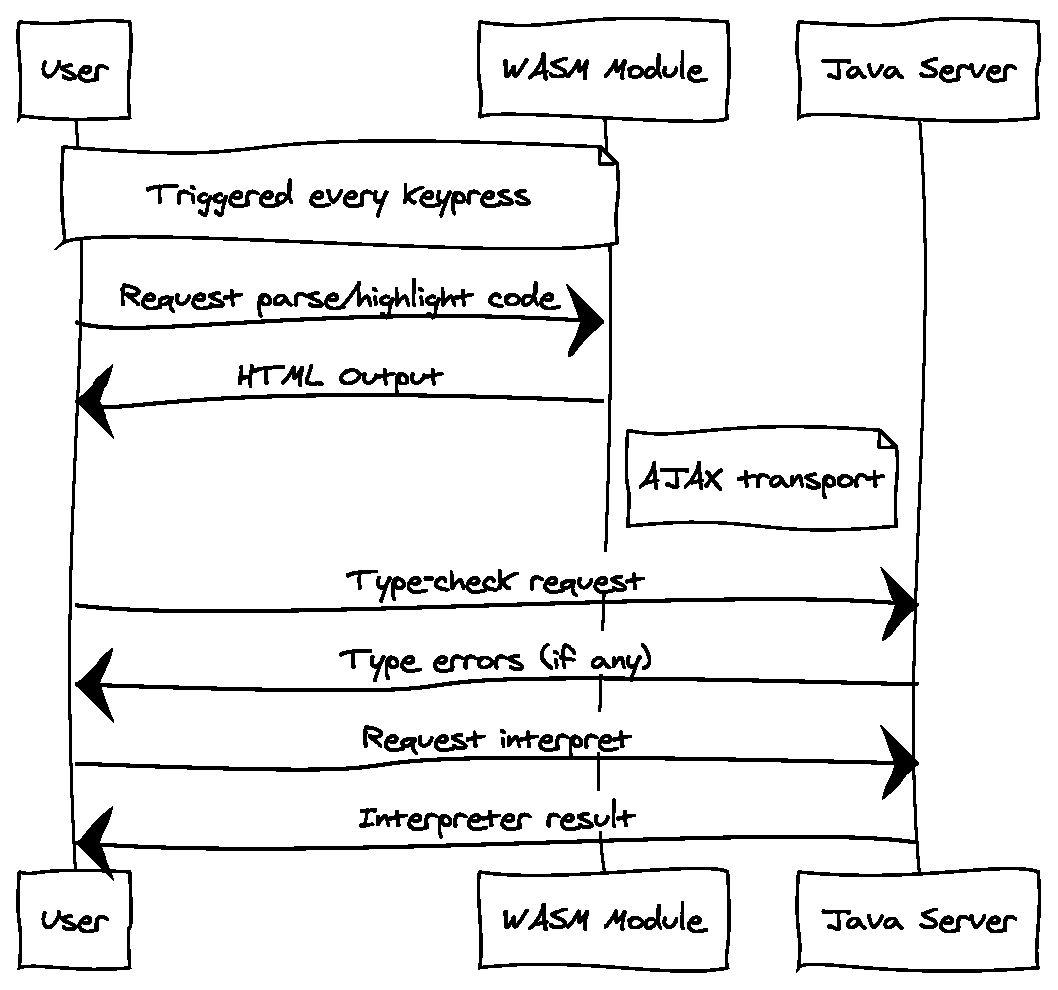
\includegraphics[width=0.5\linewidth]{seqdiagram.eps}
\end{center}

The page includes a number of different samples to demonstrate a variety of the language's features.
If the type checking is successful, the user is given the opportunity to execute their code.
The interpreter will then execute the program and print the return value of the \texttt{Main} function.

The figure below shows the web application executing a factorial program and printing the result:

\begin{center} 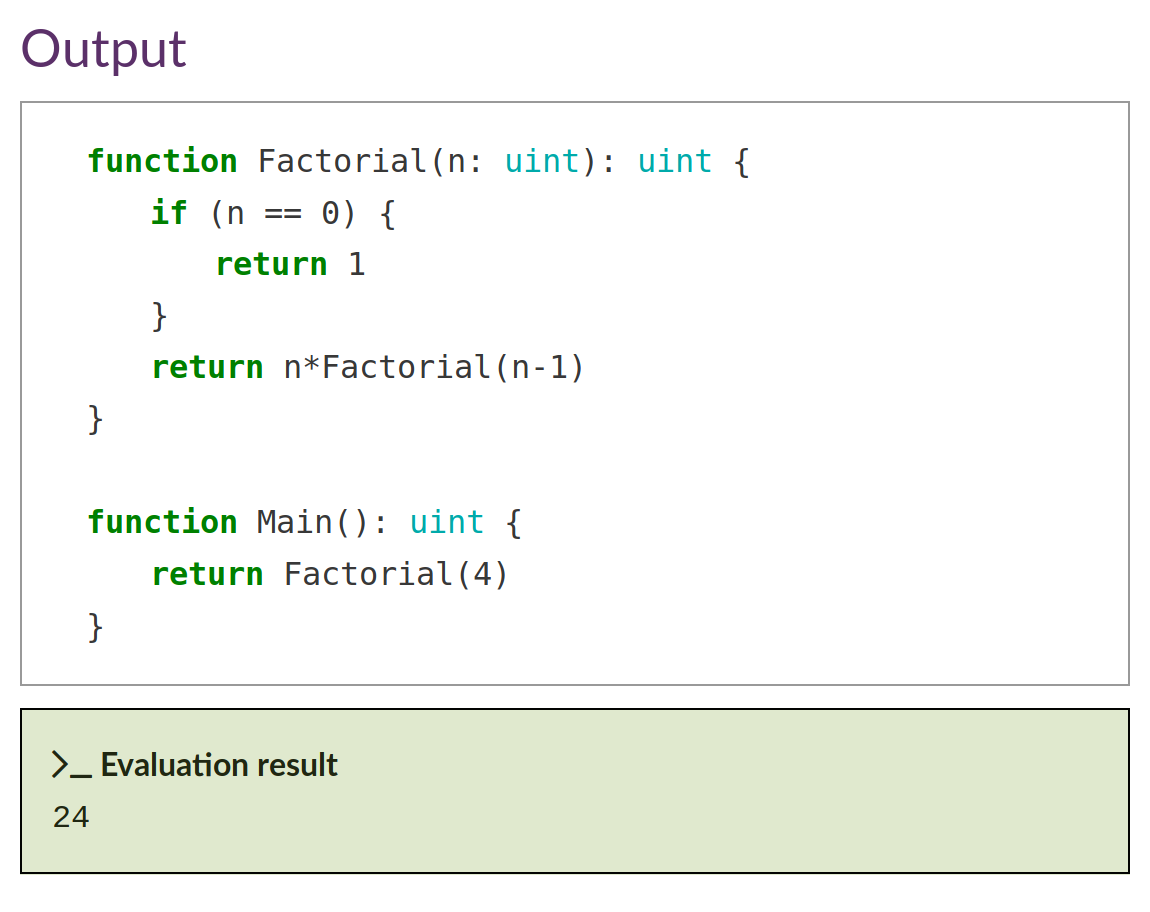
\includegraphics[width=0.75\linewidth]{interpet.png} \end{center}


\newpage
    \newgeometry{margin=0in}
    \thispagestyle{empty}

    \topskip0pt

    \tikz[remember picture,overlay] \node[opacity=1,inner sep=0pt] at (current page.center){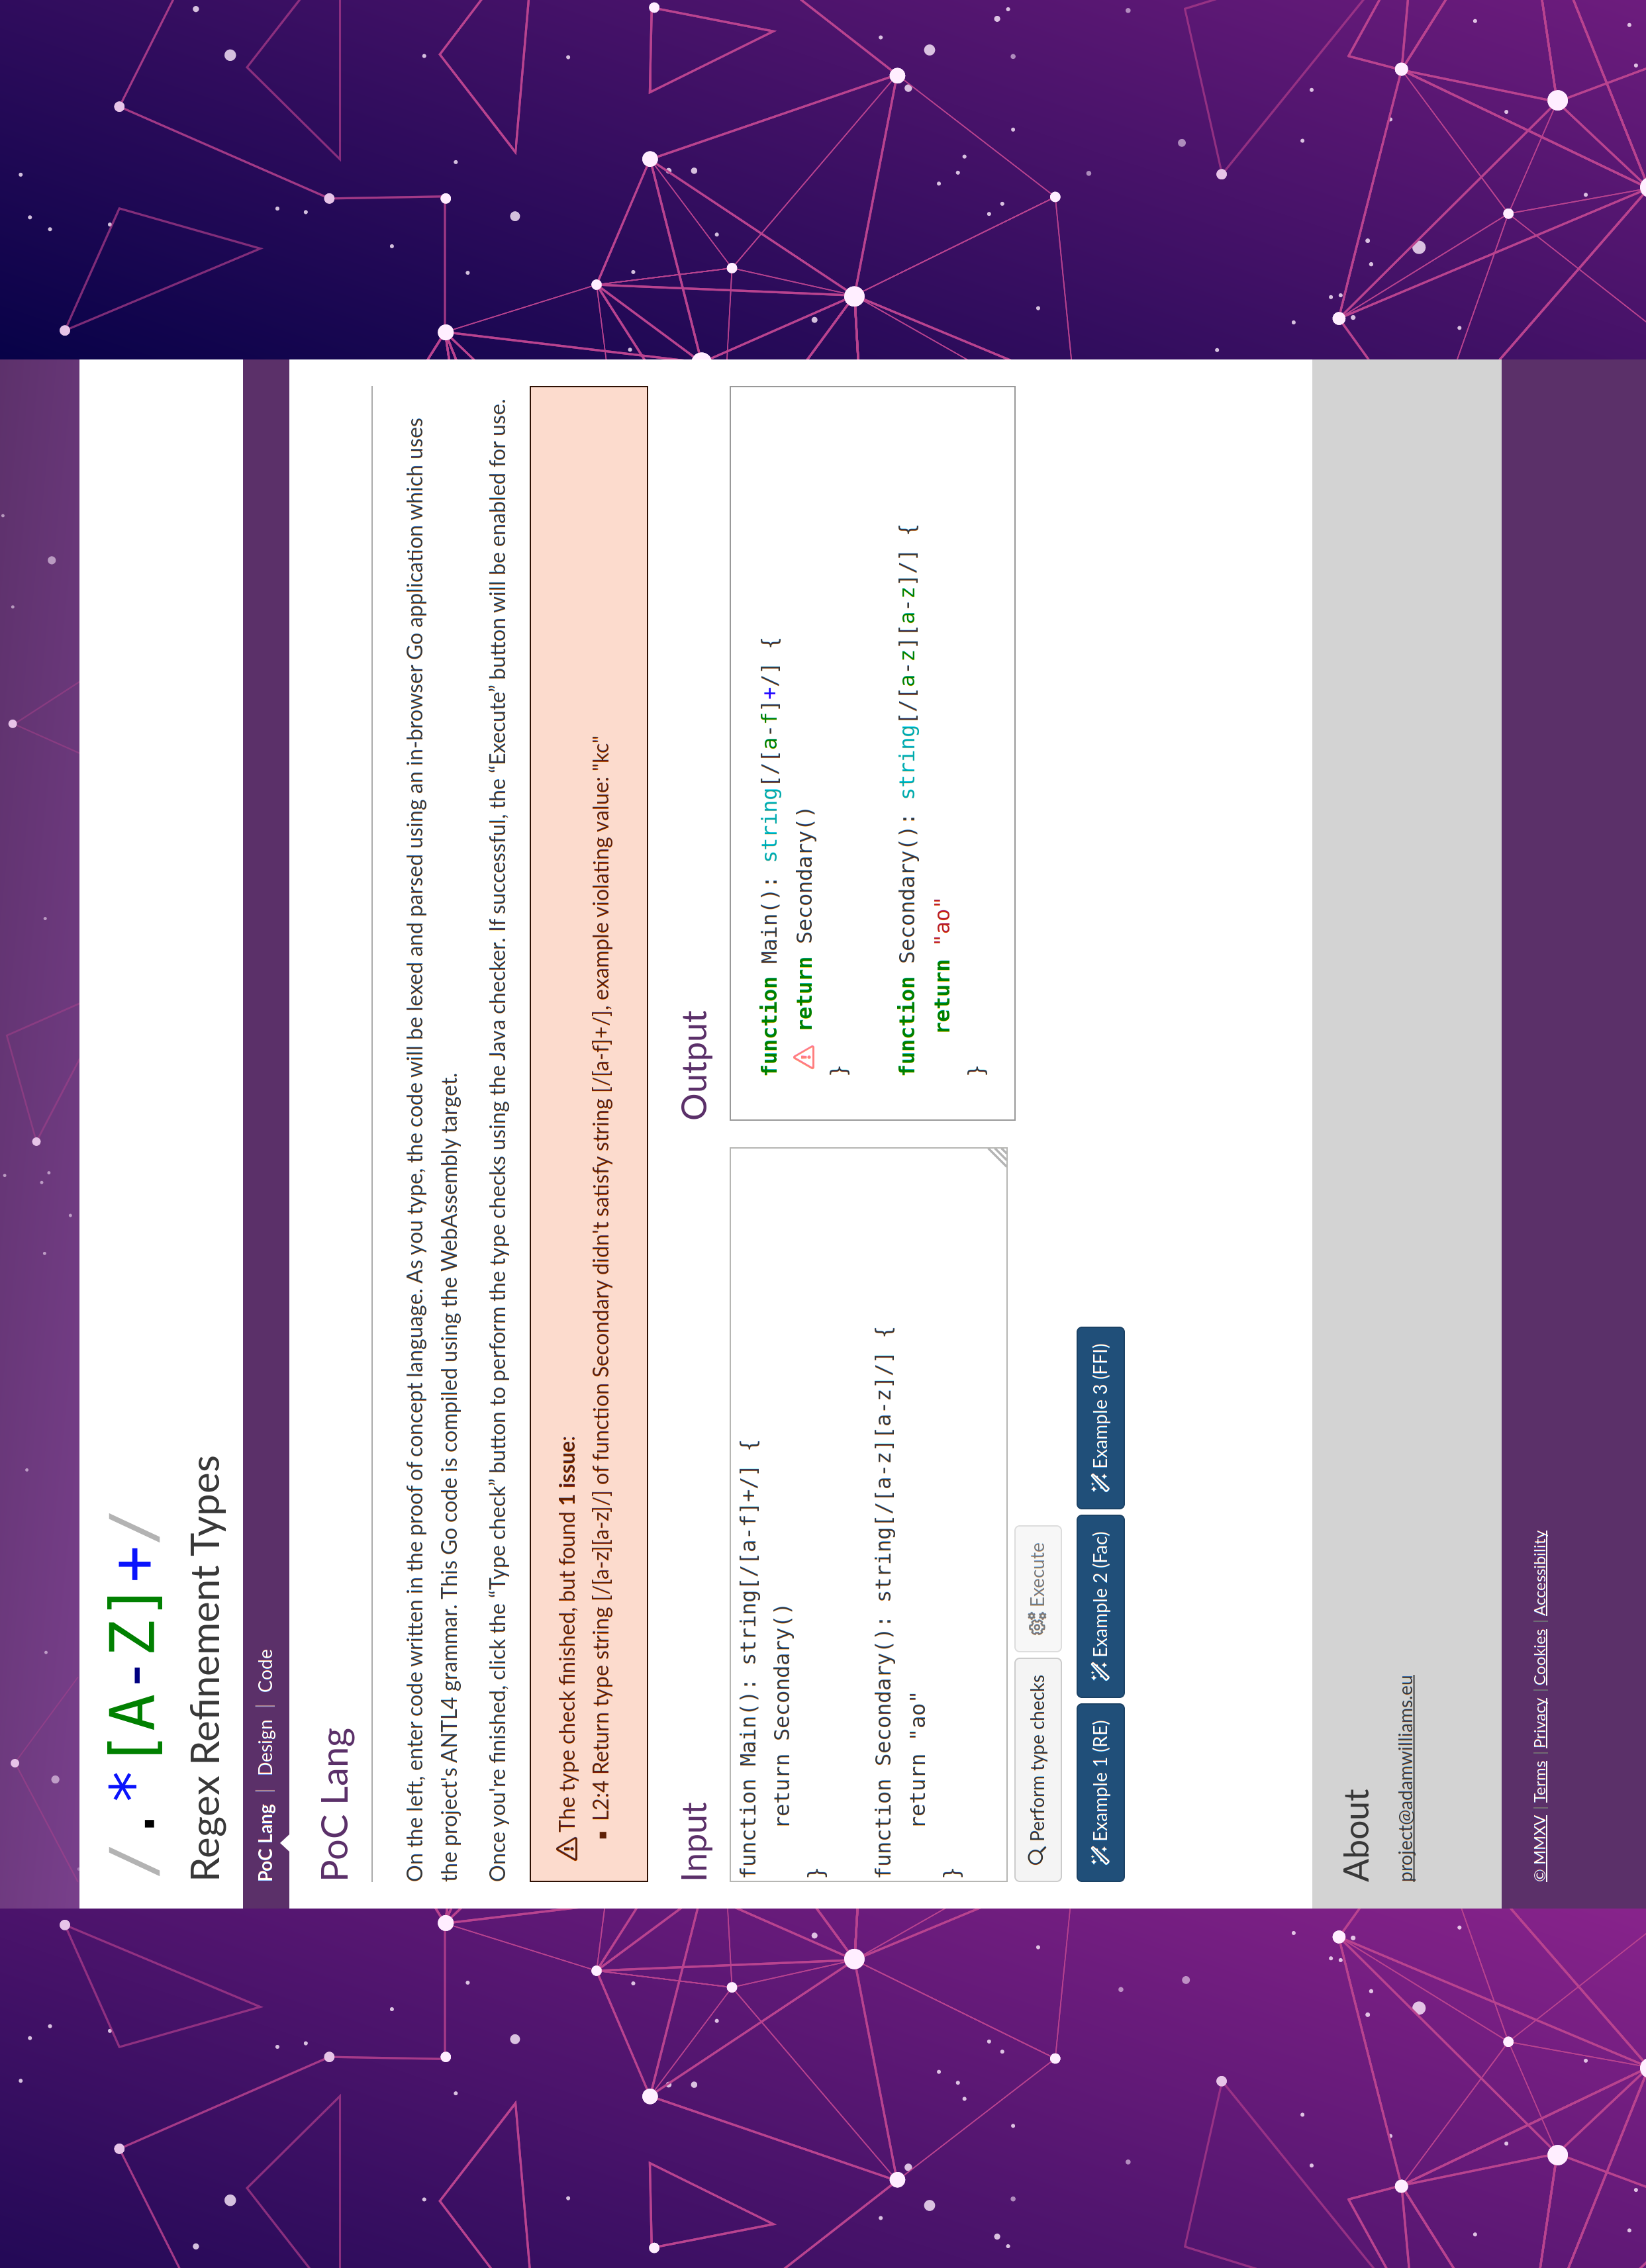
\includegraphics[width=\paperwidth,height=\paperheight]{webiface.png}};
\restoregeometry

\subsection{Rise4fun Integration}

Within Microsoft Research, the \emph{Research in Software Engineering} (RiSE) group has built a tool known as
\emph{rise4fun}.
This web based platform is an interactive sandbox where allows users interested in programming language research can
experiment with software engineering tools such as Z3, Dafny and many others.
Users can enter code in a syntax-highlighted editor and execute type-checkers and verifiers in their browser.
Results are displayed in real-time.

We natively integrate with Microsoft's Rise4fun platform to showcase our language's features and allow users to
experiment with refinement types.
Much of the web application backend could be re-used, illustrating the flexibility of the parsing and type-checking
APIs.

\begin{figure}[H]
    \begin{MyMdframed}
        \vspace{0.5em}


        \caption{\label{figure:r4f}Example of a type violation, displayed in the Rise4fun environment}
        \vspace{0.5em}
        \captionsetup{style=default}

        \begin{adjustbox}{center}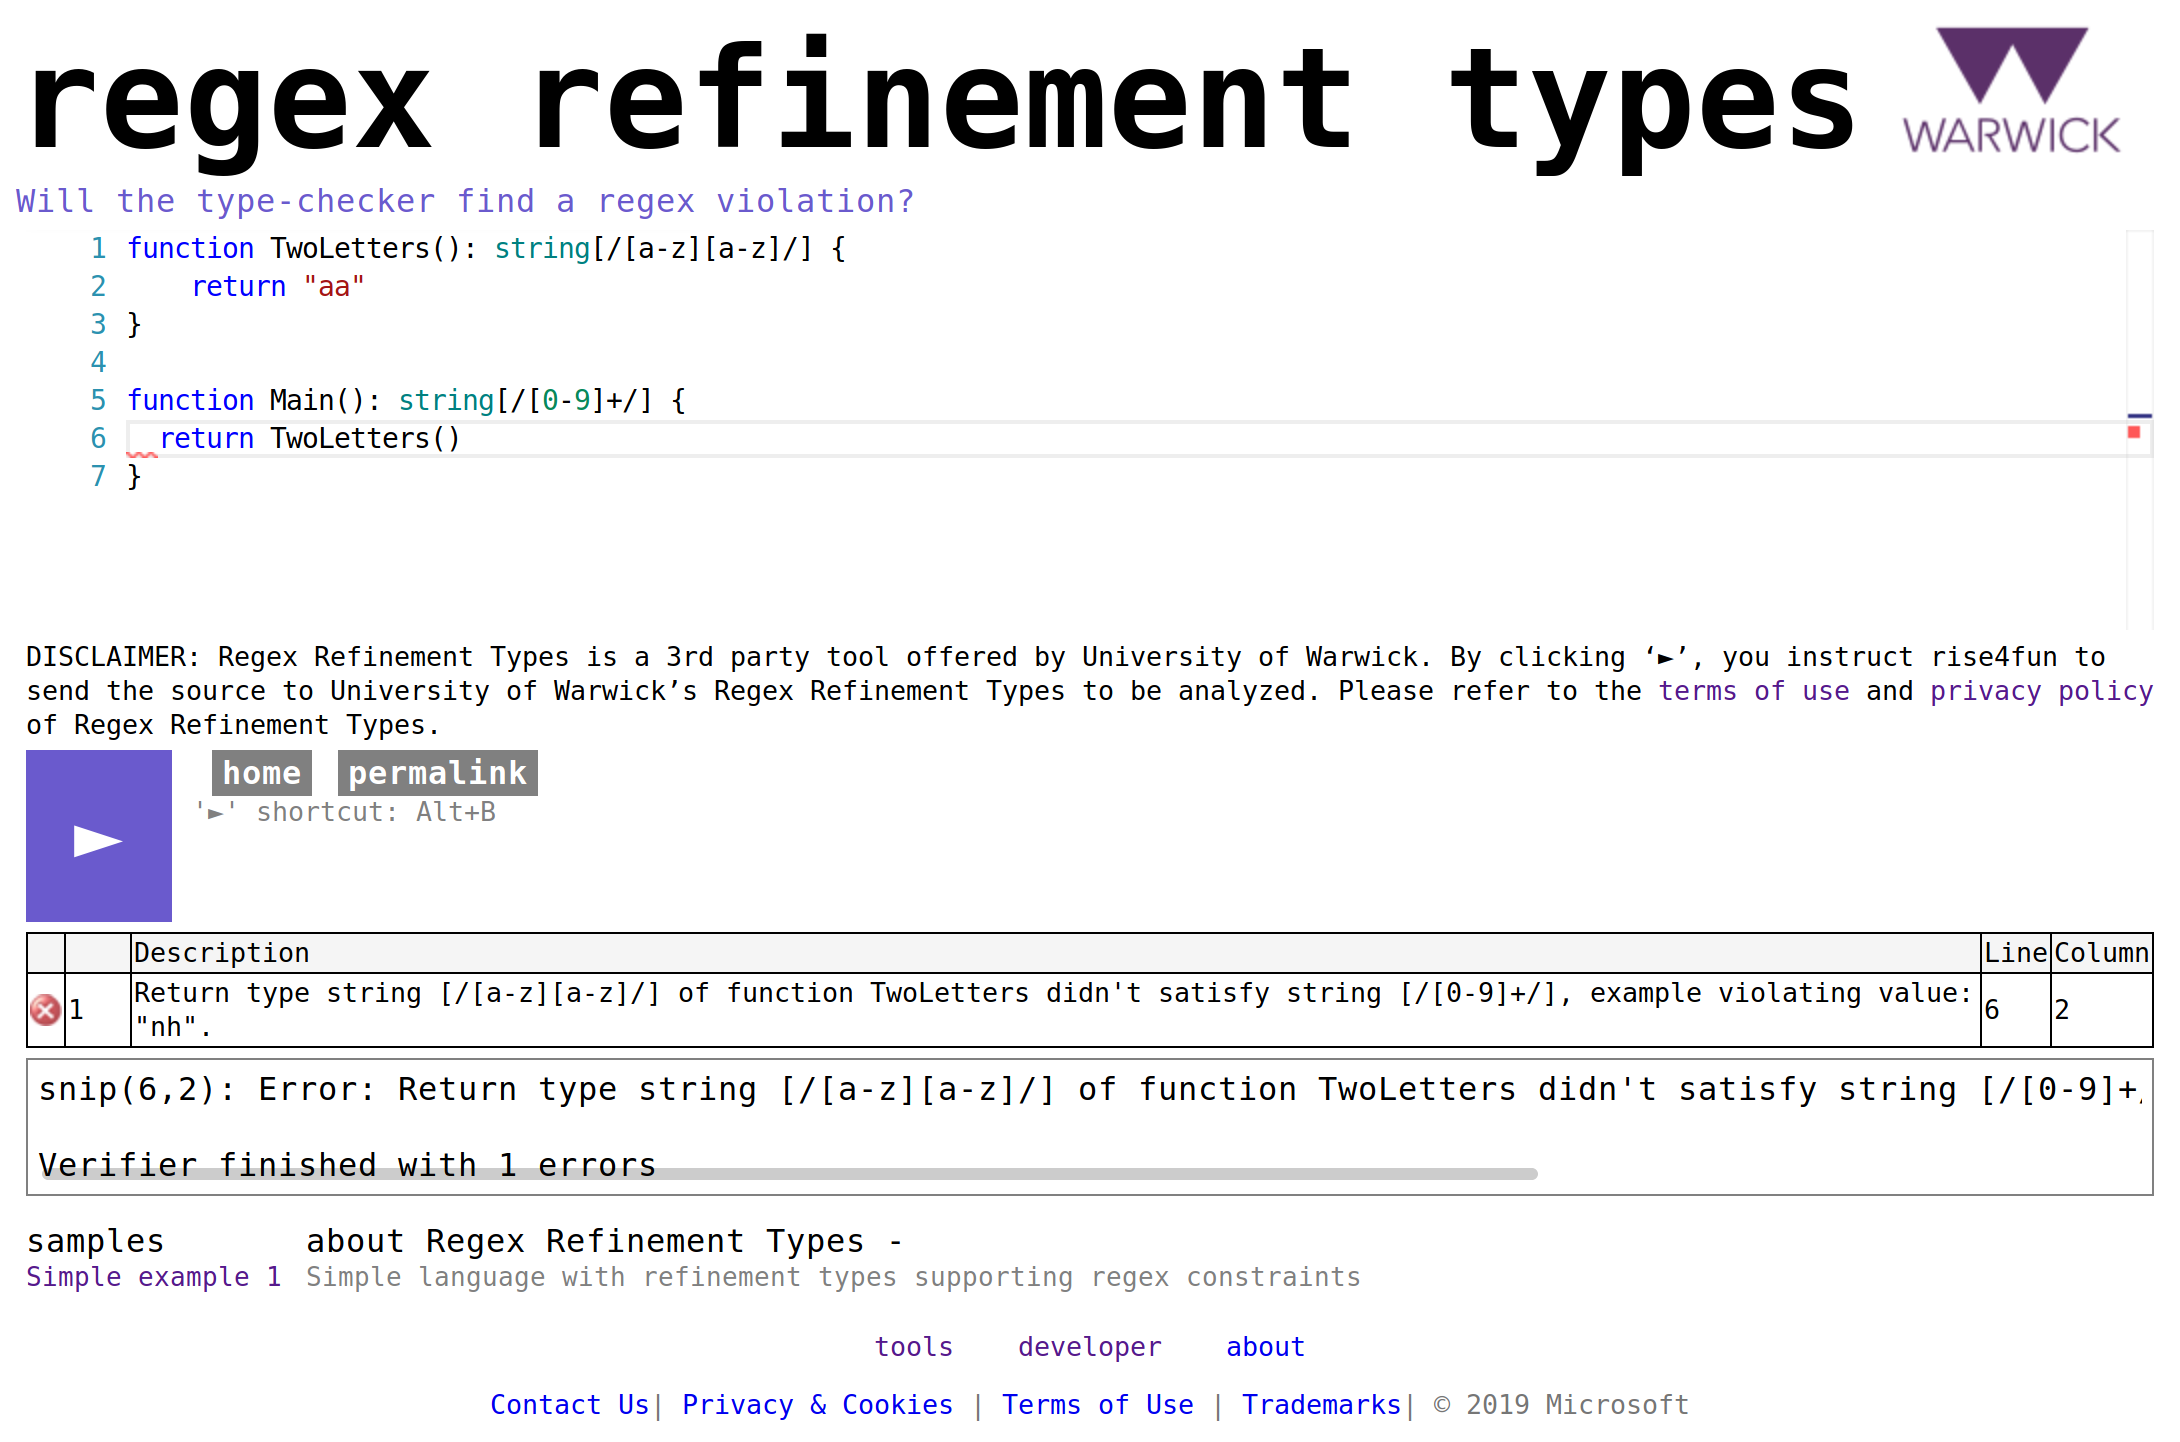
\includegraphics[width=0.9\linewidth]{rise4fun.png}\end{adjustbox}
    \end{MyMdframed}
\end{figure}

\subsection{Gradle Plugin}

We have built a Gradle plugin which enables projects to include code in the RRT language.
A build task is then provided to type-check all RRT code and report the results, failing the build if problems are
encountered.
In this way, developers can integrate the language into real-world projects.
\pagebreak[5]
Our Gradle plugin operates using the same standard directory conventions for Java software.
The root project directory includes a top-level \texttt{src/} directory which in turn contains sets for the
\texttt{main} code and for any \texttt{test} files (such as unit and integration tests).
Within each of these directories, a language directory exists for e.g. \texttt{java} or \texttt{antlr}.
We add support for a new \texttt{rrt} directory in our plugin and define an \texttt{rrt} build task:

\begin{mycodefile}{java}{Gradle plugin main class implementation}{Java}{gradle.java}\end{mycodefile}

As documented in the code, we execute type checking after the Java sources are built.
This ensures we can check the types of any project Java functions called from within the RRT sources.
When the task is executed, type checker errors are reported as in the sample below:

\termbox{
\texttt{\textcolor{term-green}{\fallbackmono{➜}} \ttfamily \textbf{\textcolor{term-dir}{examples-1} \textcolor{term-git}{(git:}\textcolor{term-branch}{master}\textcolor{term-git}{)}} ./gradlew build}\\
\textcolor{id7-ruby-red}{\texttt{\textbf{> Task :rrt} FAILED}}\\
\texttt{type.txt: L6:6 string didn't satisfy string [/A-Za-z+/], example violating value: ""}\\
~\\
\textcolor{id7-ruby-red}{\texttt{FAILURE: Build failed with an exception.}}\\
\texttt{* What went wrong:}\\
\texttt{Execution failed for task ':poc'.}\\
\texttt{> The type check failed!}\\
~\\
\texttt{* Try:\\
Run with \textbf{--stacktrace} option to get the stack trace.
Run with \textbf{--info} or \textbf{--debug} option to get more log output.
Run with --scan to get full insights.}\\
~\\
\textcolor{id7-ruby-red}{\texttt{BUILD FAILED in 9s}}
}

\section{Foreign Function Interface}

The FFI discussed earlier is implemented within the interpreter using Java's reflection.
We also use reflection to perform type checking at compile-time by ensuring that all Java code is compiled and present
on the classpath \emph{prior} to the Gradle plugin invoking the type-checking process.

We attempt to map types to their Java counterparts in an intuitive manner:

\begin{description}
    \item[uint] Can map to the primitive types (long, int, short or byte) or their boxed equivalents (Long, Integer etc.) as required.
    \item[bool] Maps to boolean or the boxed equivalent, Boolean.
    \item[string] Maps to the String type.
\end{description}

Note that types lose their refinement information as soon as they cross the FFI boundary.
This is an unfortunate necessity for compatibility with existing code, though alternative ``container objects'' were
considered.

Java function call expressions are preceded with an exclamation-mark \texttt{!} and require a fully qualified
package, class and method name.
Methods must be static and accessible (i.e. not marked with a restrictive access control modifier).

\section{Implementation Challenges}

As briefly discussed above, a number of challenges were encountered during the implementation process:

\begin{itemize}
    \item Initial type-checking work had used the JavaSMT API layer for abstracting over direct Z3 usage,
          allowing the underlying SMT solver to be swapped out with no code changes. Unfortunately,
    this library did not offer any abstractions for working with string theory solvers and so whilst it was
    possible to implement a prototype for integer refinements, it was necessary to swap out the library and use
    Z3 directly in order to implement string regular expression refinements.
    \item Bindings for Java that allowed Z3 to be used were not generally available and needed to be compiled from source.
    Some functions available in the C API were not exposed via the Java bindings, and it was necessary to work with
    the Z3 development team at Microsoft to add these additional functions to the Java API.
\end{itemize}

To varying extents, these issues were foreseeable, and time was scheduled to ensure that library functionality could
be thoroughly evaluated during the development process.

By using Z3 directly (despite the unavailability of bindings in binary form), we were able to make use of Z3str3 and
implement the type-checking of strings successfully.


\chapter{Testing}

We use a variety of automated and manual steps in order to test the system thoroughly.

\section{Unit Testing}

JUnit is a automated test framework for Java.
38 individual passing JUnit test methods are implemented to provide test coverage for the project.
These tests cover the broad areas described below:

\begin{description}
    \item[Parsing] Tests for simple syntactically valid and invalid programs, as well as parser regression tests for functions that were incorrectly parsed during development and subsequently fixed.
    \item[AST construction tests] Ensuring that programs are consistently parsed into the same, correct AST representation.
    \item[Simple type checks] Such as returning a string from a function marked as returning a string.
    \item[Other checks] Including function/variable re-declaration.
    \item[Integer refinement types] As described above, constraint violations for integer inequalities.
    \item[Regexp refinement types] As described above, constraint violations for regular language membership.
    \item[AST interpreter tests] Ensuring that the interpreter correctly evaluates expressions and statements within the AST.
\end{description}

The entire test suite can be executed using a Gradle task:

\termbox{
\texttt{\textcolor{term-green}{\fallbackmono{➜}} \ttfamily \textbf{\textcolor{term-dir}{PocLang} \textcolor{term-git}{(git:}\textcolor{term-branch}{master}\textcolor{term-git}{)}} ./gradlew test --rerun-tasks}\\\\

\textcolor{term-green}{\textbf{\texttt{BUILD SUCCESSFUL}}} \texttt{in 18s}\\
\texttt{5 actionable tasks: 5 executed}
}

Most Java development environments also incorporate a graphical test overview, as illustrated in figure \ref{fig:unittests}.
This enables tests to be executed immediately after any respectable changes in the codebase, leading to greater confidence in its correctness.
These tests were particularly useful when the grammar underwent changes because adding new language constructs often impacted how existing code would be parsed.


\begin{figure}
	\begin{MyMdframed}
		\vspace{0.5em}


		\caption{\label{fig:unittests} Passing unit tests shown in the IntelliJ IDEA integrated development environment}
		\vspace{0.5em}
		\captionsetup{style=default}
		\centering 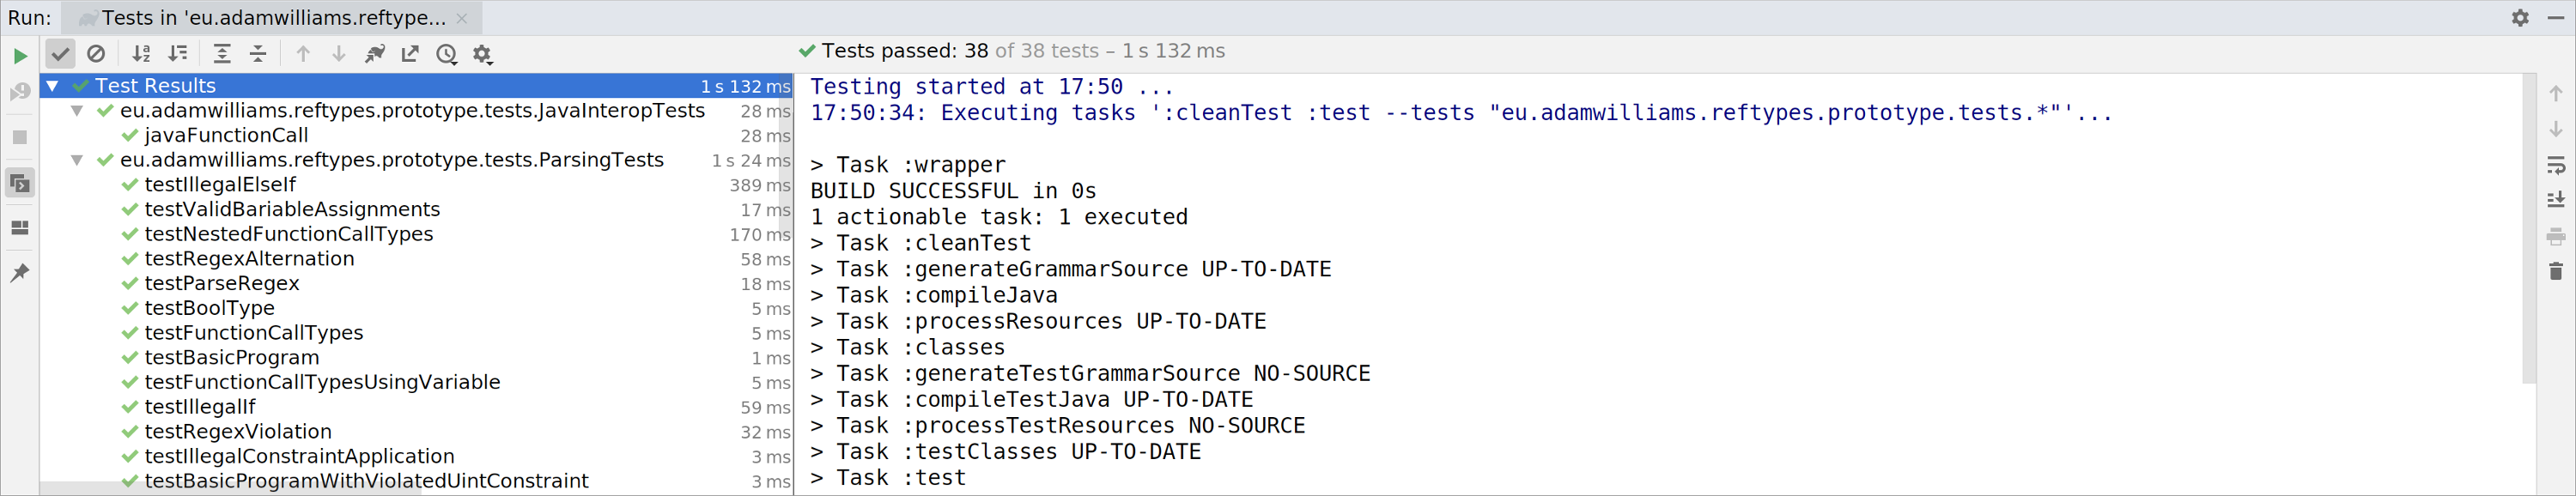
\includegraphics[width=\linewidth]{results.png}

	\end{MyMdframed}
\end{figure}

Throughout the project, the concept of test-driven development was kept in mind.
Not every change involved a test being written before it was implemented, but for important parts of the codebase this approach made sense to ensure test coverage was in place early on and to provide confidence in correctness of an implementation.


\section{Integration Testing}

We include a range of integration tests to verify the system works end-to-end.
This comprises ensuring that programs parse, type checking works as expected and the interpreter yields the correct result.
In contrast to the unit tests, which generally test specific components in isolation, the motivation behind the integration tests is to ensure that components work together correctly.
These tests can unearth new issues which would otherwise not have been detected.

\begin{mycodefile}{java}{\label{code:integration:1}Testing the Java foreign function interface with an end-to-end test}{Java}{integration.java}
In this test, we begin with a string representing a program which calls and returns a native Java function.
We parse this program, type check it and then execute it.
Throughout, we ensure that the behaviour matches our expectations and that the final result is correct.
\end{mycodefile}

\section{Manual Testing}

Automated tests go some of the way to ruling out major bugs in an application, but we feel it is still necessary to manually test software after substantial changes.
Test cases should be chosen with knowledge of the implementation in order to try and expose mishandling of edge cases, or problems with adversarial input.

As an example, applications often exhibit buggy behaviour around \emph{boundary conditions} which can be caused by off-by-one errors or use of incorrect operators.
We use test cases for integer refinements to ensure the type checker works as expected for values that fall just inside/outside of the domain of values accepted by each type.

The web interface is also more convenient to test manually.
Whilst there are some tools which are able to render pages and compare screenshots to detect e.g. layout regressions, it can be difficult to implement such tests and keep them up to date.
We find it more time-effective to manually test the web application in a variety of browsers on different devices.
Design and layout issues are usually immediately apparent.
The built-in samples are used to provide some representative programs for testing purposes, covering:

\begin{itemize}
    \item Tests for the interpreter, involving computation of the factorial.
    \item Tests for the type checker, involving integer refinements.
    \item Tests for the type checker, involving incompatible regular expression refinements.
\end{itemize}


\chapter{Evaluation}

Using the motivating examples described earlier in section \ref{subsec:examples} and a series of modifications,
we have explored the effectiveness of existing security tooling and its ability to:

\begin{itemize}
    \item Detect that the code presents a potential risk to security
    \item Correctly report, taking into account any and all validation code, whether an issue is exploitable
\end{itemize}

We have found that tooling is generally able to flag potential security vulnerabilities, but is prone to reporting
false-positives where regular-expression based validation is already in place and prevents exploitation.

\section{SQL Injection}

With our motivating example discussed in section \ref{subsec:examples}, we can observe that FindBugs is able
to correctly detect code vulnerable to SQL injection:

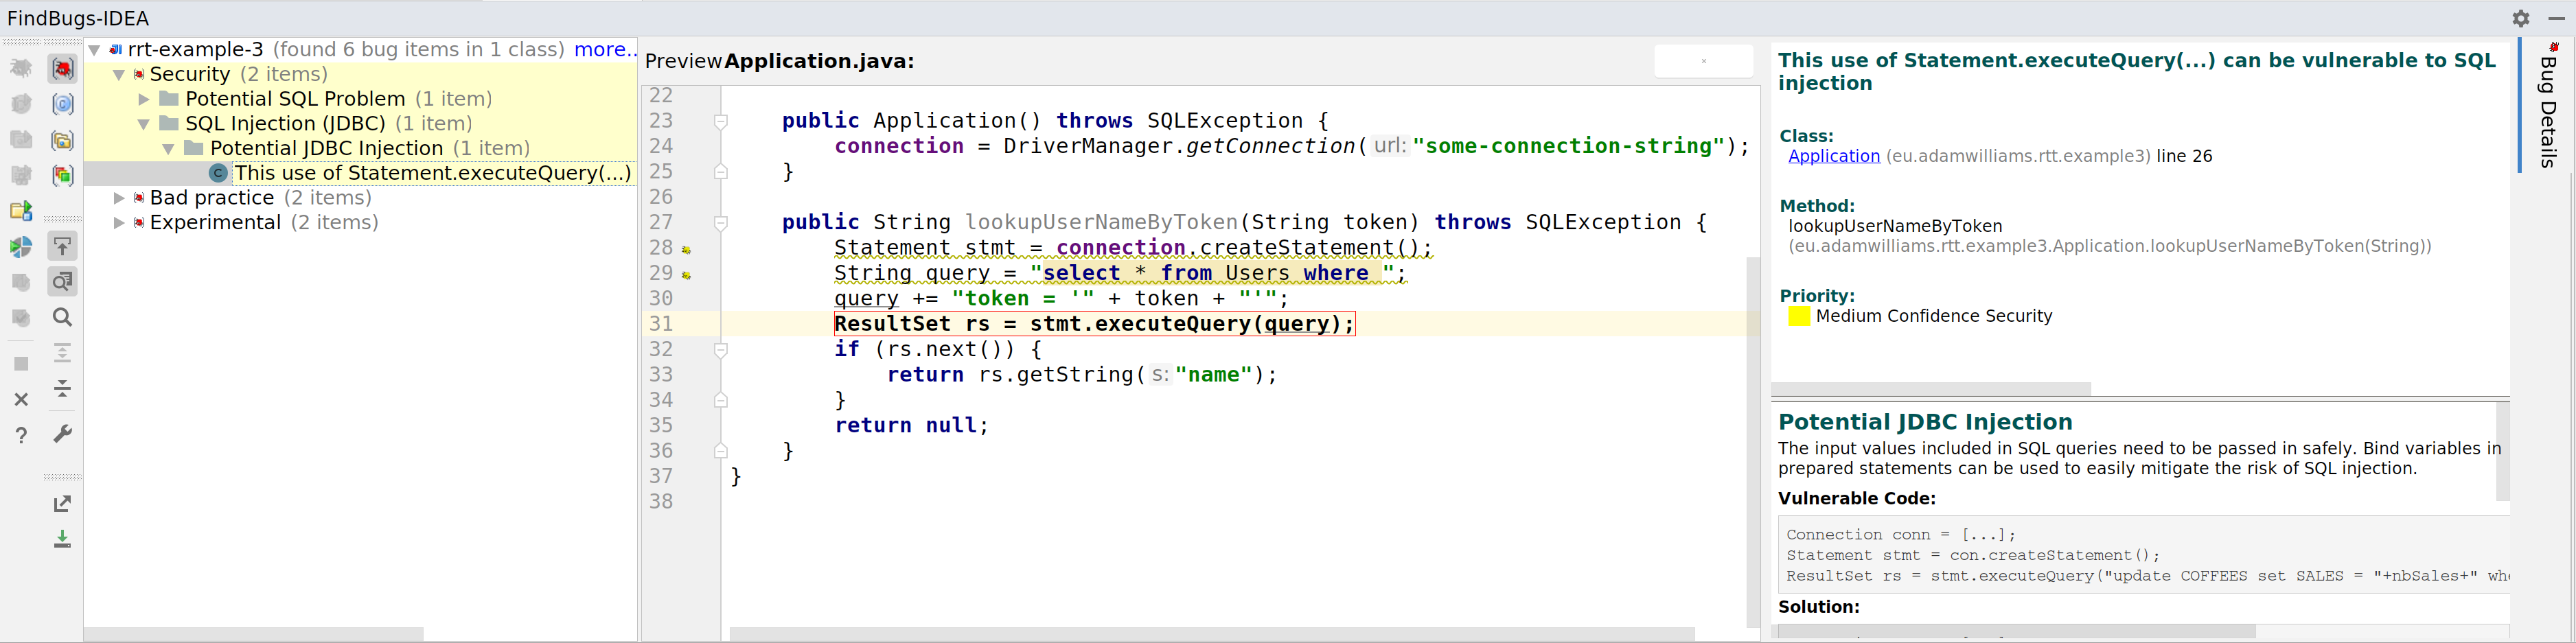
\includegraphics[width=\linewidth]{findbugs-eval.png}

If we modify this code to introduce a regular expression check at the start of the method body, it will no longer
be possible to exploit the vulnerability:

\mintinline{java}{if (!token.matches("^[a-z0-9]+$")) return null;}

However, the FindBugs rule does not take this validation into account--and the rule continues to flag up the method
as harbouring a potential security vulnerability.

We can wrap this method with one written in the RRT prototype language and take advantage of the Java foreign-function
interface by simply calling the existing Java function.
This is a simple approach which minimises the amount of work required to start benefiting from refinement types.

\begin{mycodefile}{rrtlex.py:RrtLexer -x}{Wrapping an existing Java function to use refinement types}{RRT}{sqli-wrap.rrt}
    \vspace{0.5em}

    Here, the RRT program calls a static Java method on class \texttt{Application} in package \texttt{package.java}.
    In a real application, such a static method would use a connection pool or some other means to acquire a
    database connection, and then issue the query as normal.
\end{mycodefile}

By exclusively calling the wrapper function we gain assurance that it will not be possible for input that exploits
the SQL injection vulnerability to pass to the function.

We can check this by calling the wrapper function with a known-bad input (here, as a simple string literal):

\mintinline{rrtlex.py:RrtLexer -x}{LookupUsernameByToken("' or 1=1 --")}

The type checker correctly detects this violation:

\termbox{
\texttt{\textcolor{term-green}{\fallbackmono{➜}} \ttfamily \textbf{\textcolor{term-dir}{examples-1} \textcolor{term-git}{(git:}\textcolor{term-branch}{master}\textcolor{term-git}{)}} ./gradlew build}\\
\textcolor{id7-ruby-red}{\texttt{\textbf{> Task :rrt} FAILED}}\\
\texttt{sqli-wrap.txt: L6:23 string didn't satisfy string [/[a-z0-9]+/], example violating value: "' or 1=1 --"}\\
}

When all function calls pass permissible values to the \texttt{LookupUsernameByToken}, the build will pass because
there is no exploitable security issue presented by the code.
In this way, we avoid the false positive that would have been generated with the FindBugs tool.

\section{LDAP Injection}

An attempt was made to evaluate the C\# \emph{Security Code Scan} security tool and determine if it would exhibit
similar behaviour to FindBugs--that is, reporting the existence of a potential vulnerability but not using regular
expression (or other) validation to determine if the vulnerability is actually exploitable or not.

A fresh .NET Framework project was created using the code discussed in section \ref{ex:ldapi}, and the tool was
installed.
The project provides a set of \emph{Roslyn Analysers} which are supported in a variety of different development
environments.

\begin{figure}[H]
    \begin{MyMdframed}
        \vspace{0.5em}

        \caption{\label{figure:ra}Roslyn Analysers provided by the Security Code Scan project}
        \vspace{0.5em}
        \captionsetup{style=default}
        \begin{adjustbox}{center}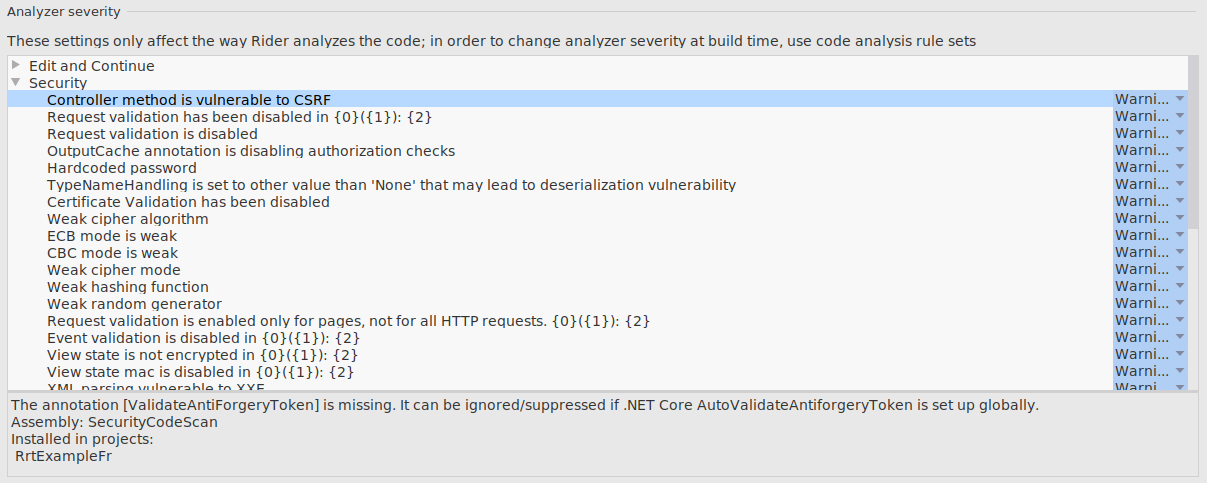
\includegraphics[width=0.6\linewidth]{analysers.png}\end{adjustbox}
    \end{MyMdframed}

\end{figure}

These analysers can in-theory be run on-demand:

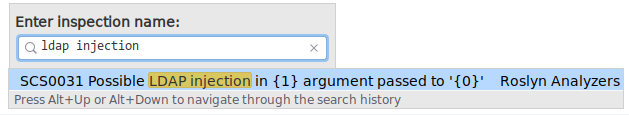
\includegraphics[width=0.6\linewidth]{scs-ldap.png}

Unfortunately, the inspection did not detect any problematic code with the unmodified example from section
\ref{ex:ldapi}.
This is disappointing, because the code showcases a textbook LDAP injection vulnerability.
It is unclear if the IDE is at fault or the inspection is too narrowly-scoped to detect this problem.

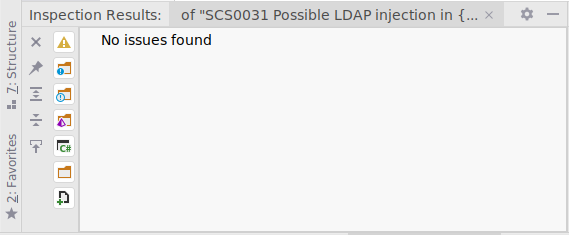
\includegraphics[width=0.5\linewidth]{no-issues-found.png}

Nevertheless, a Java implementation of the LDAP code could be wrapped in a similar way to the previous example,
accepting only user codes in the form of \texttt{/u[0-9]+/} (based on the naming scheme used in the directory).

\begin{minted}{rrtlex.py:RrtLexer -x}
function QueryUserSurname(universityId: string[/u[0-9]+/]): string {
    return !java.Ldap.queryReturnAttr("(&(objectclass=user)(cn="+universityId+")", "sn")
}
\end{minted}

The type-checker would ensure that only valid user codes would ever be passed to the \texttt{QueryUserSurname} function.

\chapter{Conclusions}

This project is a success.
We have designed and implemented a proof-of-concept language to support regular expression refinement types,
demonstrating that it is feasible to implement type checking for such a language by formulating type compatibility
as an SMT problem and using a modern SMT solver.

Using a series of test cases, we have shown that regular expression membership violations are correctly detected
and reported in a short amount of time that would not unduly affect project build performance.
Using the motivating examples discussed in section \ref{subsec:examples}, we have shown that use of regular expression
refinement types would be an effective defence in depth measure and reduce false positives compared to existing security
tooling.

We have developed a variety of interfaces to enable experimentation with our language, including a web application.
Finally, we have developed tooling to integrate our language into existing projects using an industry-standard build
system and added support for bi-directional interoperability with existing Java Virtual Machine (JVM) code.

Of the objectives discussed in section 1, all core objectives set for the project were met.
One additional `stretch' objective, which involved adding support for a language such as Scala, was not met.
This remains as possible future work as discussed below.

\section{Future work}
Our language is relatively basic, and there exist many opportunities for future work in this area.
We discuss a few possible directions for future research below.

\subsection{Non-regular expressions}

As highlighted in section \ref{sec:pls}, the standard library within many programming languages supports an extension to traditional, formal regular expressions.
A theory solver which supported these expressions would be interesting to see, and enable use of advanced features such as back-references and
.NET's balancing group definitions.

This would need to be implemented as part of an extension to an existing SMT solver framework.

\subsection{Language expansion}

Our proof of concept language is primitive by design, and only implements a small number of types.
Future development could add additional types, support for e.g. generics/parametric polymorphism, object-oriented
programming constructs and other modern programming language features.

\subsection{Imperative language integration}

In this project, we have shown a restricted proof-of-concept programming language.
It is likely that the concepts we have designed and implemented could be used to extend an existing, popular programming
language such as Java, C\# or Scala.

Many of these languages have a general mechanism to ``tag'' fields, local variables and methods with additional metadata
which can then be accessed either at runtime or compile-time.
For example, Java supports @-annotations which can be made visible at runtime, using \emph{reflection}.
This metadata mechanism could be used to specify regular expression refinements which could then be checked by an
external static analysis tool using the techniques we have described.
This would likely aid with developer adoption.

\titleformat{\chapter}[display]
{\normalfont \sffamily \Huge  \color{id7-aubergine}}
{}{0pt}{}[]

\bibliographystyle{agsm}
\bibliography{bibliography}

\appendix

\chapter{Project Specification}
\label{project:spec}
\section*{Introduction}

Within information security, entire classes of application vulnerabilities arise due to problematic user input handling \citep{christey2007vulnerability}.
This covers cross-site scripting (XSS), injection (SQL, LDAP, etc.), insecure
deserialisation and file inclusion vulnerabilities -- all of which are regularly discovered in major software products.

There are many existing products that aim to detect problems within an application. \citet{sadowski2018lessons} describe the benefits of static analysis tooling deployed within Google which allow checks for common issues to be performed as part of the compilation process. The authors explain one of the main challenges with developer adoption as \emph{trustworthiness} ``users do not trust to results due to, say, false positives`` and highlight the importance of reporting issues early: ``survey participants deemed 74\% of the issues flagged at compile time as real problems, compared to 21\% of those found in checked-in code''.

In the context of application security, tooling can be broadly categorised into the two broad areas of DAST (dynamic application security testing) and SAST (static application security testing) tooling. SAST tooling can analyse a codebase at rest and lends itself to generating much more immediate results that can take the entire codebase into account. DAST tooling allows for assessment from a black-box perspective but is much more limited. Research into the effectiveness of DAST-based scanning tools by \citet{doupe2010johnny} drew the conclusion that commonly available tools of this kind often failed to crawl more complex parts of an application which resulted in decreased coverage from a security perspective.

Existing static analysis tools can provide useful warnings that help prevent introduction of vulnerabilities.
In the .NET ecosystem, tools such as \emph{Roslyn Security Guard} can detect e.g. injection vulnerabilities by tainting
user input and then using information flow analysis -- first described in \cite{denning1977certification} -- to
determine when unsafe input is passed to a dangerous \emph{sink} function \citep{rosylynsecguard}.
Of course, this approach is limited.
All user input is deemed unsafe by virtue of being user input and prior validation (as is commonly performed using
regular expressions) is not taken into account when deciding if an alert needs to be raised or not.
This leads to false positive reports where a program is secure by virtue of already performing validation to prevent a
vulnerability.

The main objective of this project is to explore the use of a type system which uses regular-expression based refinement
types applied to user input.
A refinement type in the context of a type system is a type that is subject to a particular predicate \citep[p.
207]{benjaminpierce2002}.
By considering flow of data that belongs to a refinement type for a particular pattern, it will be possible to make
inferences about vulnerabilities that may be present in a codebase based on declared safe argument types.
Use of refinement types in this way provides for a more informed evaluation of a particular risk than base types alone
and should therefore enable reporting of fewer false positive issues.

\begin{listing}[H]
    \begin{minted}{javascript}
function LookupName(userId: /[A-Za-z0-9]+/): string {
    var name: string = GetNameByUserId(userId); // safe
    GetNameByUserId("'; DROP TABLE users;"); // type error
    return name;
}

function GetNameByUserId(query: /[^`"']+/): /[A-Za-z ]+/ {
    // database lookup..
}
    \end{minted}
    \caption{Example code illustrating a potential syntax. \texttt{userId} and \texttt{query} use the refinement type.}
\end{listing}
\section*{Objectives}



\subsubsection*{Primary Objectives}

\begin{itemize}
    \item Formalise a type system that supports types predicated with a regular expression pattern that elements of the refined type will satisfy (be matched by).

    \begin{itemize}
        \item Explore the consequences of typical string operations (e.g. concatenation) and define the type of their return value when applied to elements of the regular expression type.

        \item At minimum, this should allow for simple functions to be declared that can safely accept/return a particular regular expression input\footnote{As a simplified example, an \texttt{unsafe\_shell\_exec} function might safely be able to accept any input that matches \texttt{\textasciicircum{}[\textasciicircum{}\textasciigrave{}]\textdollar{}}}.

        \item Evaluate the rate of false positives when compared to existing static analysis
    \end{itemize}

    \item Implement such a type system that can guarantee type safety, built against a simplified proof-of-concept language.
    \begin{itemize}
        \item Test the implementation against a variety of test cases. The testing strategy should make use of automated unit tests, and manual system testing considering both general expected input as well as any relevant ``edge-cases'' that need to be handled.
    \end{itemize}
\end{itemize}

\subsubsection*{Additional Objectives}

\begin{itemize}
    \item Apply the theory explored in the primary phase of the project to produce a type analysis tool which works against type annotations applied to a commonly-used language such as C\# or Scala. This tooling could be integrated into an IDE or CI pipeline.
\end{itemize}

\textit{}\infobox{Primary objectives are expected to be completed during the lifetime of the project. Additional objectives are identified as potential goals to pursue beyond the original scope of the project, if time permits.}

\section*{Schedule}

\arrayrulecolor{white}
\begin{table}[H]

    \centering
    \rowcolors{1}{id7-sky-blue-tint}{lightgrey}
    \begin{tabular}[t]{|p{5.5cm}|p{10cm}|}
        \hline
        \rowcolor{id7-sky-blue}
        {\color[HTML]{FFFFFF} \sffamily \textbf{Time Window}} & {\color[HTML]{FFFFFF} \sffamily \textbf{Work}} \\ \hline
        October \nth{1} -- October \nth{14} & Specification completion, research into prior related works. Study of elementary programming language and type system theory (e.g. simply typed $\lambda$-calculus, SLam). \\ \hline
        October \nth{15} -- October \nth{28} & \parbox[t]{10cm}{Begin writing background for report, work on formalisation of regular expression refinement type.\\\textcolor{id7-ruby-red}{\textbf{Deadline}: CS353 presentation, \nth{24} October}}\vspace{0.4em} \\ \hline
        October \nth{29} -- November \nth{11} & Explore and document properties of type system. Begin implementation of ideas to produce a concrete proof-of-concept. \\ \hline
        November \nth{12} -- November \nth{25} & Completion of progress report, continued implementation work. \\ \hline
        November \nth{26} -- December \nth{9} & \parbox[t]{10cm}{Testing of implemented proof-of-concept.\\\textcolor{id7-ruby-red}{\textbf{Deadline}: CS915 coursework, \nth{26} November}}\vspace{0.4em} \\ \hline
        December \nth{10} -- January \nth{6} & Slack time (to use if behind schedule, else to make a start on year scheduled in 2019). \\ \hline
        January \nth{7} -- January \nth{20} & \parbox[t]{10cm}{Finalise testing of implementation, write-up test cases.\\\textcolor{id7-ruby-red}{\textbf{Deadline}: CS324 coursework}}\vspace{0.4em} \\ \hline
        January \nth{21} -- February \nth{3} & Evaluate false positive rates against existing systems based exclusively on taint tracking. \\ \hline
        February \nth{4} -- February \nth{17} & Report work, project presentation preparation \\ \hline
        February \nth{18} -- March \nth{3} & Project presentation preparation, report work \\ \hline
        March \nth{4} -- March \nth{17} & Project presentation delivery, report finalisation. \\ \hline
    \end{tabular}
    \caption{Projected work by time period. Deadlines for other modules included where known.}
    \label{schedule}
\end{table}

Table \ref{schedule} provides a breakdown of the project time into periods for each fortnight, along with the expected work to be completed. A meeting will be scheduled for each week to discuss progress and any road-blocks that arise with the project supervisor

\section*{Methodology}

\subsection*{Software Engineering}

This project includes an element of software engineering. Namely, the design and implementation of a proof of concept language which supports a type system incorporating regular expression refinement types.

This implementation work will be carried out in an Agile fashion to fit in with the short timescales inherent to the project and allow for greater flexibility. Time periods in the schedule which involve development work will be treated as a number of week-long development sprints with priorities formalised prior to the commencement of each period. Progress will be reviewed in weekly supervision meetings.

Testing will be automated via the use of unit testing to ensure that specific components function according to their specification in isolation. Where appropriate, integration and system testing can be used to test the solution as a whole (for example, an entire program as a test case would fit into this part of the testing process).

\subsection*{Evaluation}

Towards the end of the implementation phase, the false positive rate of the proof of concept tool should be compared with that of existing static analysis tooling based on taint tracking alone.

Logically equivalent test cases should be built for each tool under evaluation in the necessary programming language. Both safe and unsafe function invocations should be included in each test case for completeness.

\section*{Resources and risks}


The project is reliant on a number of resources. Use of these resources is subject to the risks outlined in table \ref{rr}. These risks should be evaluated and managed to minimise any potential impact on the project.

\arrayrulecolor{white}
\begin{table}[H]

    \centering
    \rowcolors{1}{id7-sky-blue-tint}{lightgrey}
    \begin{tabular}[t]{|p{5.5cm}|p{4cm}|p{7cm}|}
        \hline
        \rowcolor{id7-sky-blue}
        {\color[HTML]{FFFFFF} \sffamily \textbf{Resource}} & {\color[HTML]{FFFFFF} \sffamily \textbf{Applicable risk(s)}} &
        {\color[HTML]{FFFFFF} \sffamily \textbf{Impact}} \\ \hline
        \parbox[t]{5cm}{\textbf{VCS hosting: GitHub}\\Storing and tracking code and report changes\\} & Loss of availability due to outage & Minimal, \emph{git} is decentralised so copy of files always available locally and at off-site backup \\ \hline
        \parbox[t]{5cm}{\textbf{Report authoring: \LaTeX}\\Writing and compiling the report, tracking bibliography} & Obsolescence & Unlikely, TeX tooling has been used for decades. Even if particular packages ceased working, the bulk of the content would still be accessible as plain text. \\ \hline
        \parbox[t]{5cm}{\textbf{C\# analysis: Roslyn library}\\Fulfilling the additional objective by analysing C\# code} & Loss of availability due to license change & Minimal. Even if Roslyn's OSS status changes, there is no requirement to integrate with C\#, other languages would illustrate the potential just as well. This would also not impact a primary project objective. \\ \hline
        \parbox[t]{5cm}{\textbf{Self}\\Project work} & Illness, coursework deadlines & Minimised by scheduled slack time and identification of applicable coursework deadlines. \\ \hline
    \end{tabular}
    \caption{Resources and associated risks. \label{rr}}
\end{table}


\section*{Legal, social, ethical and professional issues}

As a project with some security motivation, it is possible that legal, social, ethical and professional issues will arise. In particular, evaluation of existing static analysis tooling must be performed with care to ensure that use of any particular external test cases is permitted by the \emph{Copyright, Designs and Patents Act 1988} within the UK.

Additionally, in order to comply with the \emph{Computer Misuse Act 1990}, any static analysis of external code should only be conducted with permission.  Discovered issues should be disclosed responsibly.

\end{document}
